% Options for packages loaded elsewhere
\PassOptionsToPackage{unicode}{hyperref}
\PassOptionsToPackage{hyphens}{url}
%
\documentclass[
]{book}
\usepackage{amsmath,amssymb}
\usepackage{lmodern}
\usepackage{iftex}
\ifPDFTeX
  \usepackage[T1]{fontenc}
  \usepackage[utf8]{inputenc}
  \usepackage{textcomp} % provide euro and other symbols
\else % if luatex or xetex
  \usepackage{unicode-math}
  \defaultfontfeatures{Scale=MatchLowercase}
  \defaultfontfeatures[\rmfamily]{Ligatures=TeX,Scale=1}
\fi
% Use upquote if available, for straight quotes in verbatim environments
\IfFileExists{upquote.sty}{\usepackage{upquote}}{}
\IfFileExists{microtype.sty}{% use microtype if available
  \usepackage[]{microtype}
  \UseMicrotypeSet[protrusion]{basicmath} % disable protrusion for tt fonts
}{}
\makeatletter
\@ifundefined{KOMAClassName}{% if non-KOMA class
  \IfFileExists{parskip.sty}{%
    \usepackage{parskip}
  }{% else
    \setlength{\parindent}{0pt}
    \setlength{\parskip}{6pt plus 2pt minus 1pt}}
}{% if KOMA class
  \KOMAoptions{parskip=half}}
\makeatother
\usepackage{xcolor}
\IfFileExists{xurl.sty}{\usepackage{xurl}}{} % add URL line breaks if available
\IfFileExists{bookmark.sty}{\usepackage{bookmark}}{\usepackage{hyperref}}
\hypersetup{
  pdftitle={Time Series and Forecasting: A Project-based Approach with R},
  pdfauthor={Arthur Small},
  hidelinks,
  pdfcreator={LaTeX via pandoc}}
\urlstyle{same} % disable monospaced font for URLs
\usepackage{color}
\usepackage{fancyvrb}
\newcommand{\VerbBar}{|}
\newcommand{\VERB}{\Verb[commandchars=\\\{\}]}
\DefineVerbatimEnvironment{Highlighting}{Verbatim}{commandchars=\\\{\}}
% Add ',fontsize=\small' for more characters per line
\usepackage{framed}
\definecolor{shadecolor}{RGB}{248,248,248}
\newenvironment{Shaded}{\begin{snugshade}}{\end{snugshade}}
\newcommand{\AlertTok}[1]{\textcolor[rgb]{0.94,0.16,0.16}{#1}}
\newcommand{\AnnotationTok}[1]{\textcolor[rgb]{0.56,0.35,0.01}{\textbf{\textit{#1}}}}
\newcommand{\AttributeTok}[1]{\textcolor[rgb]{0.77,0.63,0.00}{#1}}
\newcommand{\BaseNTok}[1]{\textcolor[rgb]{0.00,0.00,0.81}{#1}}
\newcommand{\BuiltInTok}[1]{#1}
\newcommand{\CharTok}[1]{\textcolor[rgb]{0.31,0.60,0.02}{#1}}
\newcommand{\CommentTok}[1]{\textcolor[rgb]{0.56,0.35,0.01}{\textit{#1}}}
\newcommand{\CommentVarTok}[1]{\textcolor[rgb]{0.56,0.35,0.01}{\textbf{\textit{#1}}}}
\newcommand{\ConstantTok}[1]{\textcolor[rgb]{0.00,0.00,0.00}{#1}}
\newcommand{\ControlFlowTok}[1]{\textcolor[rgb]{0.13,0.29,0.53}{\textbf{#1}}}
\newcommand{\DataTypeTok}[1]{\textcolor[rgb]{0.13,0.29,0.53}{#1}}
\newcommand{\DecValTok}[1]{\textcolor[rgb]{0.00,0.00,0.81}{#1}}
\newcommand{\DocumentationTok}[1]{\textcolor[rgb]{0.56,0.35,0.01}{\textbf{\textit{#1}}}}
\newcommand{\ErrorTok}[1]{\textcolor[rgb]{0.64,0.00,0.00}{\textbf{#1}}}
\newcommand{\ExtensionTok}[1]{#1}
\newcommand{\FloatTok}[1]{\textcolor[rgb]{0.00,0.00,0.81}{#1}}
\newcommand{\FunctionTok}[1]{\textcolor[rgb]{0.00,0.00,0.00}{#1}}
\newcommand{\ImportTok}[1]{#1}
\newcommand{\InformationTok}[1]{\textcolor[rgb]{0.56,0.35,0.01}{\textbf{\textit{#1}}}}
\newcommand{\KeywordTok}[1]{\textcolor[rgb]{0.13,0.29,0.53}{\textbf{#1}}}
\newcommand{\NormalTok}[1]{#1}
\newcommand{\OperatorTok}[1]{\textcolor[rgb]{0.81,0.36,0.00}{\textbf{#1}}}
\newcommand{\OtherTok}[1]{\textcolor[rgb]{0.56,0.35,0.01}{#1}}
\newcommand{\PreprocessorTok}[1]{\textcolor[rgb]{0.56,0.35,0.01}{\textit{#1}}}
\newcommand{\RegionMarkerTok}[1]{#1}
\newcommand{\SpecialCharTok}[1]{\textcolor[rgb]{0.00,0.00,0.00}{#1}}
\newcommand{\SpecialStringTok}[1]{\textcolor[rgb]{0.31,0.60,0.02}{#1}}
\newcommand{\StringTok}[1]{\textcolor[rgb]{0.31,0.60,0.02}{#1}}
\newcommand{\VariableTok}[1]{\textcolor[rgb]{0.00,0.00,0.00}{#1}}
\newcommand{\VerbatimStringTok}[1]{\textcolor[rgb]{0.31,0.60,0.02}{#1}}
\newcommand{\WarningTok}[1]{\textcolor[rgb]{0.56,0.35,0.01}{\textbf{\textit{#1}}}}
\usepackage{longtable,booktabs,array}
\usepackage{calc} % for calculating minipage widths
% Correct order of tables after \paragraph or \subparagraph
\usepackage{etoolbox}
\makeatletter
\patchcmd\longtable{\par}{\if@noskipsec\mbox{}\fi\par}{}{}
\makeatother
% Allow footnotes in longtable head/foot
\IfFileExists{footnotehyper.sty}{\usepackage{footnotehyper}}{\usepackage{footnote}}
\makesavenoteenv{longtable}
\usepackage{graphicx}
\makeatletter
\def\maxwidth{\ifdim\Gin@nat@width>\linewidth\linewidth\else\Gin@nat@width\fi}
\def\maxheight{\ifdim\Gin@nat@height>\textheight\textheight\else\Gin@nat@height\fi}
\makeatother
% Scale images if necessary, so that they will not overflow the page
% margins by default, and it is still possible to overwrite the defaults
% using explicit options in \includegraphics[width, height, ...]{}
\setkeys{Gin}{width=\maxwidth,height=\maxheight,keepaspectratio}
% Set default figure placement to htbp
\makeatletter
\def\fps@figure{htbp}
\makeatother
\setlength{\emergencystretch}{3em} % prevent overfull lines
\providecommand{\tightlist}{%
  \setlength{\itemsep}{0pt}\setlength{\parskip}{0pt}}
\setcounter{secnumdepth}{5}
\usepackage{booktabs}
\ifLuaTeX
  \usepackage{selnolig}  % disable illegal ligatures
\fi
\usepackage[]{natbib}
\bibliographystyle{apalike}

\title{Time Series and Forecasting:
A Project-based Approach with R}
\author{Arthur Small}
\date{Version of: 2022-03-19}

\begin{document}
\maketitle

{
\setcounter{tocdepth}{1}
\tableofcontents
}
\hypertarget{preface}{%
\chapter*{Preface}\label{preface}}
\addcontentsline{toc}{chapter}{Preface}

This document is a compilation of class notes for SYS 5581 \emph{Time Series and Forecasting}, University of Virginia, Spring, 2021.

\begin{Shaded}
\begin{Highlighting}[]
\FunctionTok{library}\NormalTok{(tidyverse)}
\end{Highlighting}
\end{Shaded}

\begin{verbatim}
## -- Attaching packages --------------------------------------- tidyverse 1.3.1 --
\end{verbatim}

\begin{verbatim}
## v ggplot2 3.3.5     v purrr   0.3.4
## v tibble  3.1.6     v dplyr   1.0.8
## v tidyr   1.2.0     v stringr 1.4.0
## v readr   2.1.2     v forcats 0.5.1
\end{verbatim}

\begin{verbatim}
## -- Conflicts ------------------------------------------ tidyverse_conflicts() --
## x dplyr::filter() masks stats::filter()
## x dplyr::lag()    masks stats::lag()
\end{verbatim}

\begin{Shaded}
\begin{Highlighting}[]
\FunctionTok{library}\NormalTok{(fpp3)}
\end{Highlighting}
\end{Shaded}

\begin{verbatim}
## -- Attaching packages -------------------------------------------- fpp3 0.4.0 --
\end{verbatim}

\begin{verbatim}
## v lubridate   1.8.0     v feasts      0.2.2
## v tsibble     1.1.1     v fable       0.3.1
## v tsibbledata 0.4.0
\end{verbatim}

\begin{verbatim}
## -- Conflicts ------------------------------------------------- fpp3_conflicts --
## x lubridate::date()    masks base::date()
## x dplyr::filter()      masks stats::filter()
## x tsibble::intersect() masks base::intersect()
## x tsibble::interval()  masks lubridate::interval()
## x dplyr::lag()         masks stats::lag()
## x tsibble::setdiff()   masks base::setdiff()
## x tsibble::union()     masks base::union()
\end{verbatim}

\hypertarget{preface-1}{%
\chapter*{Preface}\label{preface-1}}
\addcontentsline{toc}{chapter}{Preface}

This document contains class notes and other materials related to SYS 5581 \emph{Time Series and Forecasting} at the University of Virginia.

\hypertarget{readings-and-references}{%
\section*{Readings and references}\label{readings-and-references}}
\addcontentsline{toc}{section}{Readings and references}

\hypertarget{time-series}{%
\subsection*{Time series}\label{time-series}}
\addcontentsline{toc}{subsection}{Time series}

FPP3 = Hyndman, R.J., \& Athanasopoulos, G. \citeyearpar{robjhyndmanForecastingPrinciplesPractice2021} \href{https://otexts.com/fpp3/}{\emph{Forecasting: principles and practice, 3rd edition}}, OTexts: Melbourne, Australia. OTexts.com/fpp3

TFS = {[}these notes{]}

\hypertarget{statistics-with-r}{%
\subsection*{Statistics with R}\label{statistics-with-r}}
\addcontentsline{toc}{subsection}{Statistics with R}

\hypertarget{data-science-with-r-general}{%
\subsection*{Data science with R, general}\label{data-science-with-r-general}}
\addcontentsline{toc}{subsection}{Data science with R, general}

R4DS = Wickham, Hadley, and Garrett Grolemund, \href{https://r4ds.had.co.nz/}{\emph{R for Data Science}}

TSDS = Carrie Wright, Shannon E. Ellis, Stephanie C. Hicks and Roger D. Peng, \href{https://jhudatascience.org/tidyversecourse/}{\emph{Tidyverse Skills for Data Science}}

Tibshirani, Ryan, \href{https://www.stat.cmu.edu/~ryantibs/statcomp/}{Statistics 36-350 \emph{Statistical Computing}}, Carnegie-Mellon University, Fall 2019

\hypertarget{other-references-on-zotero}{%
\subsection*{Other references on Zotero}\label{other-references-on-zotero}}
\addcontentsline{toc}{subsection}{Other references on Zotero}

A variety of other references to resources on time series and forecasting are gathered in \href{https://www.zotero.org/groups/2555186/uva_engineering_time_series_and_forecasting/library}{the Zotero library for this course}.

\hypertarget{acknowledgements}{%
\section*{Acknowledgements}\label{acknowledgements}}
\addcontentsline{toc}{section}{Acknowledgements}

These notes are organized using the \textbf{bookdown} package \citep{R-bookdown}, which was built on top of R Markdown and \textbf{knitr} \citep{xie2015}.

\hypertarget{course-syllabus}{%
\chapter*{Course Syllabus}\label{course-syllabus}}
\addcontentsline{toc}{chapter}{Course Syllabus}

title: ``SYS 5581 Time Series and Forecasting''
author: ``Instructor: Arthur Small''
date: ``University of Virginia Engineering, Spring 2021''

\emph{Class meetings:} MW 09:30-10:45 a.m. online via Zoom

\emph{Office Hours:} MW 11:00 a.m.-12:30 p.m. online via Zoom (subject to change). Sign up in advance for a 45-minute session via the Collab ``Sign Up'' tool. If you cannot make any scheduled time, please contact the instructor via email to schedule an appointment. Meetings online via Zoom: \url{https://virginia.zoom.us/my/arthursmalliii}

\emph{Web Resources:}

\begin{itemize}
\tightlist
\item
  \href{https://collab.its.virginia.edu}{Collab class site}, for basic course information, assignments, office hours sign-up, links to online textbook and other resources.
\item
  \href{https://github.com/uva-eng-time-series-sp21}{Github class site}, for posting and sharing code.
\item
  Zoom, for class sessions, recordings, and office hours.
\end{itemize}

\hypertarget{course-description}{%
\section*{Course Description}\label{course-description}}
\addcontentsline{toc}{section}{Course Description}

The course is designed to introduce graduate students and advanced undergraduates in engineering to time series and forecasting. The course will not include a deep exploration of theory. Rather, the goal is for students by the end to be able to analyze time series data competently, as part of their work designing and working with engineered systems.

In addition to learning theory, each student will undertake a semester-long research project. Ideally, this project will relate closely to the student's own dissertation research, professional practice, or other domain application that interests them. My hope is that these projects could form the basis for subsequent research papers, dissertation chapters, or other professional work products, for interested students.

The course will, therefore, be structured primarily as a \emph{workshop}: the ultimate goal is to help you to create a professionally presented report. Our workflow will, therefore, be subject to revision, according to my judgement of how best to use our time to help you produce a professional report.

The course outline is divided into two major sections. First, we will introduce the theory, with examples. In the later part of the semester, we will focus on workshopping your projects in progress.

Important: class readings are subject to change, contingent on mitigating circumstances and the progress we make as a class. Students are encouraged to attend lectures and check the course website for updates.

\hypertarget{prerequisites}{%
\subsection*{Prerequisites}\label{prerequisites}}
\addcontentsline{toc}{subsection}{Prerequisites}

Students should have taken at least one rigorous intermediate course in probability and statistics. They should be comfortable with the representation of uncertain information in the form of probability distributions, with conditional probabilities, and with other such foundational concepts.

In addition, to carry out the data analyis, the student should have at least ability be able to code, in some general-purpose language. For this course, we will work in R, focusing on specialized packages for working with time series data and generating forecasts.

\hypertarget{expectations}{%
\subsection*{Expectations}\label{expectations}}
\addcontentsline{toc}{subsection}{Expectations}

Each student will make a presentation on their data analysis project. Students will be evaluated based on their performance in these presentations and on their final project, on occasional short quizzes; and on their contributions inside and outside of class towards helping other students.

\hypertarget{readings}{%
\subsection*{Readings}\label{readings}}
\addcontentsline{toc}{subsection}{Readings}

The primary text for the course will be \href{https://otexts.com/fpp3/}{\emph{Forecasting: Principles and Practice}, 3rd ed.} by
Rob J. Hyndman and George Athanasopoulos. This resource is available for free online and is linked from the Collab site. The text includes example code in R, and covers several useful R packages related to time series and forecasting.

Additional readings including relevant articles will be provided as the course progresses. The choice of readings will depend in part on student interests, as conveyed through their choice of projects.

\hypertarget{course-objectives}{%
\subsection*{Course Objectives}\label{course-objectives}}
\addcontentsline{toc}{subsection}{Course Objectives}

\begin{enumerate}
\def\labelenumi{\arabic{enumi}.}
\item
  Students will learn the foundations of time series and forecasting.
\item
  Students will gain the experience of building statistical models of time series, and models for forecasting, and will learn how to evaluate their performance.
\item
  Students will learn the concepts and practice of \emph{reproducible research}, in the course of preparing a research paper.
\item
  Students will gain experience in making presentations and in preparing a polished research article.
\end{enumerate}

\hypertarget{grading-policy} of your grade will be determined by quizzes designed to test your understanding of the theoretical concepts introduced in class. This quiz will delivered at roughly the mid-point of the semester. It will be open-book and open-notes, outside of class. You will have multiple days to complete it. The quiz will not be designed to be especially challenging: the goal is to give you the opportunity to synthesize your understanding of core concepts, in preparation for developing your data analysis for your research project.
\item
  \textbf{10\%} of your grade will be determined by your performance in one in-class presentation based on your project. These presentations will be scheduled when you are, in the judgement of the instructor, far enough along to do so.
\item
  \textbf{10\%} of your grade will be determined by your contributions to assist other students. These contributions can come through class participation, by making useful contributions in online forums (Github), or through other means that add value to the group experience.
\item
  \textbf{70\%} of your grade will be determined by your performance on your final project. The development of the project will include multiple iterations, each with an associated deliverable:

  \begin{itemize}
  \tightlist
  \item
    An initial Concept Note.
  \item
    A more developed Project Proposal.
  \item
    A first working draft of your final project paper.
  \item
    A final complete draft of your project paper.
  \end{itemize}
\end{itemize}

Details of these staged intermediate deliverables will be forthcoming. The final product should be a polished professional paper that meets academic standards regarding format, quality, and integrity.

\hypertarget{attendance-policy}{%
\subsection*{Attendance Policy}\label{attendance-policy}}
\addcontentsline{toc}{subsection}{Attendance Policy}

Regular attendance is very much in your pedagogic interest. However, it is up to you whether to attend in person or to view recorded class sessions afterwards.

\hypertarget{communications-protocols-including-emails-and-office-hours}{%
\subsection*{Communications protocols, including emails and office hours}\label{communications-protocols-including-emails-and-office-hours}}
\addcontentsline{toc}{subsection}{Communications protocols, including emails and office hours}

I prefer to avoid using email to communicate with students about class matters. For substantive questions about course materials and concepts, please use class time, office hours, or meetings by appointment. Please use email only for brief clarifying questions, or to set up appointments.

\hypertarget{academic-dishonesty-policy}{%
\subsection*{Academic Dishonesty Policy}\label{academic-dishonesty-policy}}
\addcontentsline{toc}{subsection}{Academic Dishonesty Policy}

Don't cheat. Don't plagiarize. Don't present someone else's work as your own.

\hypertarget{disabilities-policy}{%
\subsection*{Disabilities Policy}\label{disabilities-policy}}
\addcontentsline{toc}{subsection}{Disabilities Policy}

Together with the University of Virginia, I am committed to assuring that all students have the full opportunity to benefit from the course regardless of their disability status. If you have a disability that may require accommodations, please see the instructor early in the semester to work out appropriate arrangements.

\hypertarget{part-introduction-and-overview}{%
\part{Introduction and Overview}\label{part-introduction-and-overview}}

\hypertarget{intro}{%
\chapter{Introduction}\label{intro}}

Readings: FPP3, Ch. 1

\hypertarget{what-is-time-series-analysis}{%
\section{What is time series analysis?}\label{what-is-time-series-analysis}}

\hypertarget{time-series-data}{%
\section{Time series data}\label{time-series-data}}

\hypertarget{time-series-patterns}{%
\section{Time series patterns}\label{time-series-patterns}}

Examples.

\hypertarget{types-of-problems-that-are-amenable-to-time-series-analysis}{%
\section{Types of problems that are amenable to time series analysis}\label{types-of-problems-that-are-amenable-to-time-series-analysis}}

\hypertarget{time-series-and-forecasting}{%
\section{Time series and forecasting}\label{time-series-and-forecasting}}

\hypertarget{overview-of-the-course}{%
\section{Overview of the course}\label{overview-of-the-course}}

\hypertarget{project-workflow}{%
\chapter{Project workflow}\label{project-workflow}}

Readings:

\begin{itemize}
\tightlist
\item
  \href{https://otexts.com/fpp3/a-tidy-forecasting-workflow.html}{FPP3, Section 5.1}
\item
  \href{https://jhudatascience.org/tidyversecourse/model.html\#about-this-course-4}{TSDS, Sections 5.1-5.3}
\end{itemize}

Case study examples:

\begin{itemize}
\tightlist
\item
  \href{https://www.opencasestudies.org/ocs-bp-co2-emissions/}{Open Case Studies: Exploring CO2 emissions across time}
\item
  \href{https://www.opencasestudies.org/ocs-bp-air-pollution/}{Open Case Studies: Predicting Annual Air Pollution}
\end{itemize}

Steps in a time series statistical analysis:

\begin{enumerate}
\def\labelenumi{\arabic{enumi}.}
\tightlist
\item
  State your question
\item
  Acquire data and background information
\item
  Organize your data
\item
  Perform exploratory analysis of your data
\item
  Write down your model of the data generating process
\item
  If necessary: transform the model and data to make it ready for analysis
\item
  Choose an appropriate technique for estimating model parameters, consistent with your assumptions about your data generating process
\item
  Estimate model parameters
\item
  Confirm that your modeling assumptions are satisfied;
\item
  Compute measures of model quality; confirm that your model is good enough for your purpose
\item
  Use your calibrated model to address your original question.
\end{enumerate}

Examples of using your model:

\begin{itemize}
\tightlist
\item
  Generate a forecast of future events
\item
  Estimate the probability of a future event
\item
  \(\ldots\)
\end{itemize}

\hypertarget{example-problem-estimating-the-probability-of-a-weather-event}{%
\section*{Example problem: Estimating the probability of a weather event}\label{example-problem-estimating-the-probability-of-a-weather-event}}
\addcontentsline{toc}{section}{Example problem: Estimating the probability of a weather event}

A pub owner in Charlottesville plans to sell beer outside on St.~Patrick's Day, March 17. The pub owner must decide whether to arrange to rent a supplemental refrigeration system for the day.

Supplemental refrigeration offers a form of insurance. If temperatures outside on March 17 are high and the pub owner has not arranged supplemental refrigeration, she will be left with warm beer that she will have difficulty selling, leading to financial losses. Conversely, if she pays for supplemental refrigeration when temperatures are low, she will have incurred an unnecessary expense.

To decide whether to insure herself against loss, she wishes to estimate the probability distribution of temperatures on March 17.

\hypertarget{state-your-question}{%
\section{State your question}\label{state-your-question}}

\textbf{1. What is the probability that the high temperature on March 17 will exceed 23 degrees Celsius?}

\hypertarget{acquire-data-and-background-information}{%
\section{Acquire data and background information}\label{acquire-data-and-background-information}}

Get historical temperature data.

(Here, will simulate the data.)

\begin{Shaded}
\begin{Highlighting}[]
\FunctionTok{set.seed}\NormalTok{(}\DecValTok{1}\NormalTok{)       }\CommentTok{\# Keeps random data from changing each time the code is run}

\NormalTok{theta }\OtherTok{\textless{}{-}}  \DecValTok{18}      \CommentTok{\# True long{-}run average temp}
\NormalTok{sigma  }\OtherTok{\textless{}{-}}  \DecValTok{3}      \CommentTok{\# True stnd dev of temp around this mean}
\NormalTok{n      }\OtherTok{\textless{}{-}} \DecValTok{40}      \CommentTok{\# n = number of simulated historical data points}
                     \CommentTok{\# We don\textquotesingle{}t use \textquotesingle{}T\textquotesingle{} because in R language \textquotesingle{}T\textquotesingle{} = logical \textquotesingle{}TRUE\textquotesingle{}}

\NormalTok{y }\OtherTok{\textless{}{-}} \FunctionTok{rnorm}\NormalTok{(n,theta,sigma)}
\end{Highlighting}
\end{Shaded}

\hypertarget{organize-your-data}{%
\section{Organize your data}\label{organize-your-data}}

Let \(y_1, \ldots, y_T\) denote the high temperature in Charlottesville on March 17 for each of the previous \(T\) years.

\begin{Shaded}
\begin{Highlighting}[]
\FunctionTok{print}\NormalTok{(y)}
\end{Highlighting}
\end{Shaded}

\begin{verbatim}
##  [1] 16.12064 18.55093 15.49311 22.78584 18.98852 15.53859 19.46229 20.21497
##  [9] 19.72734 17.08383 22.53534 19.16953 16.13628 11.35590 21.37479 17.86520
## [17] 17.95143 20.83151 20.46366 19.78170 20.75693 20.34641 18.22369 12.03194
## [25] 19.85948 17.83161 17.53261 13.58774 16.56555 19.25382 22.07604 17.69164
## [33] 19.16301 17.83858 13.86882 16.75502 16.81713 17.82206 21.30008 20.28953
\end{verbatim}

\hypertarget{perform-exploratory-analysis-of-your-data}{%
\section{Perform exploratory analysis of your data}\label{perform-exploratory-analysis-of-your-data}}

\begin{Shaded}
\begin{Highlighting}[]
\FunctionTok{hist}\NormalTok{(y, }\AttributeTok{breaks =} \DecValTok{20}\NormalTok{, }\AttributeTok{main =} \StringTok{"Histogram of historical temperatures in degrees C"}\NormalTok{)}
\end{Highlighting}
\end{Shaded}

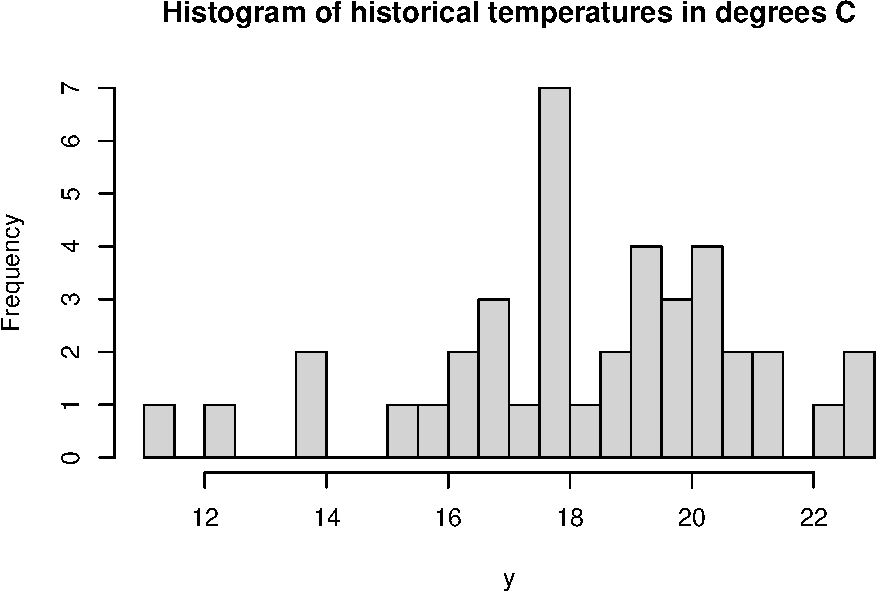
\includegraphics{graphics/unnamed-chunk-4-1.pdf}

\begin{Shaded}
\begin{Highlighting}[]
\FunctionTok{boxplot}\NormalTok{(y)}
\end{Highlighting}
\end{Shaded}

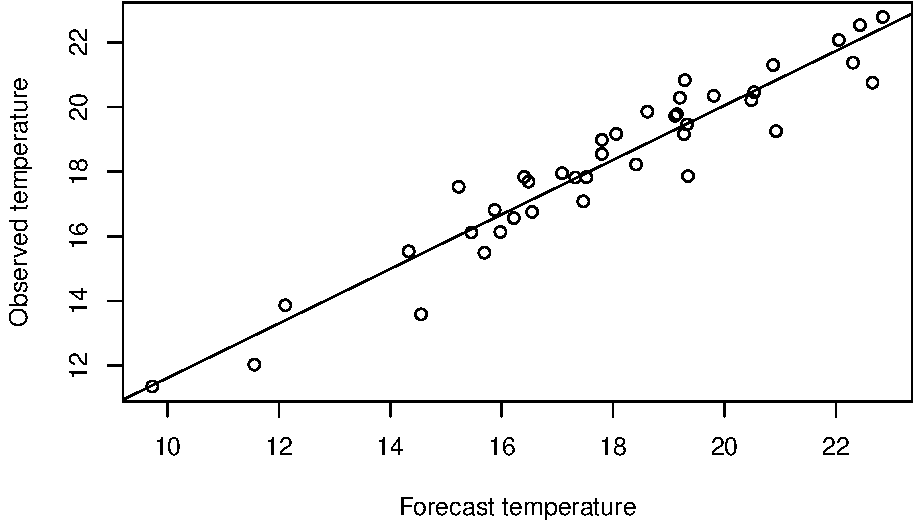
\includegraphics{graphics/unnamed-chunk-5-1.pdf}

\hypertarget{white-noise-model}{%
\section{Write down your model of the data generating process}\label{white-noise-model}}

It is supposed that these data were generated as independent, identically distributed random draws from a normal distribution: for \(t = 1, \ldots, T\),

\[y_t = \theta + \varepsilon_t\]
where \(\theta\) denotes the true but unobserved value of the long-run average temperature, and where \(\varepsilon_t \sim N(0, \sigma^2)\).

\hypertarget{comments-on-this-statistical-model-the-risk-of-model-mis-specification}{%
\subsection{Comments on this statistical model: The risk of model mis-specification}\label{comments-on-this-statistical-model-the-risk-of-model-mis-specification}}

This model asserts several substantive assumptions about the data generating process.

\begin{itemize}
\item
  The process is assumed to be \emph{stationary}. There is no upward trend over time, no long-term climate change, etc.
\item
  Temperatures are assumed to be \emph{independent} from one year to the next. In particular, there is no \emph{autocorrelation}. Knowing that one year's temperature was unusually high (say) provides no information about the likelihood that next year's temperature will also be unusually high. Inter-annual climate cycles (e.g., due to \(El\ Ni\tilde{n}o\)) are ruled out.
\item
  Temperature variations around the long-run average are assumed to be \emph{identically distributed}. This assumption rules out the possibility that variance is, say, greater when temperatures are higher than when they are lower.
\end{itemize}

And others.

In general, it is important to formulate a statistical model that accurately reflects the true characteristics of the underlying data generating process.

When your statistical model is mis-specified, your probabilistic forecast of future events are likely to stray from the true underlying probabilities. Model mis-specification can then lead to inaccurate estimates of the distribution of losses for each possible action. This error may in turn lead to selection of a sub-optimal action.

A particular problem to guard against is the possibility to underestimate the likelihood of extreme events that could cause catastrophic losses.

That said, your time on this Earth is limited. Depending on the decision problem and the stakes involved, refining your model to get sharper loss estimates may or may not be worth the bother.

A reasonable approach is to start by first writing down a simple forecasting model that appears to capture the essence of the process as you understand it. On the basis of this simple model, generate first-cut probabilistic forecasts of uncertain events. Use these to generate estimated distributions of losses for each possible action in your action set. On that basis, use the specified decision criterion to derive an initial optimal decision rule.

Then, go back and check things over more carefully. Review the realism of your statistical model, given your understanding of data generating process. Plot and examine the distribution of your prediction errors. Do your prediction errors appear to follow a pattern that matches what you would expect, given the assumptions you have made?

If you find evidence that your prediction model is mis-specified, it may be worth it to go back and refine your model, and see if you generate different results.

One very good idea is to perform a \emph{sensitivity analysis}. How sensitive are your decision recommendations and outcomes to the assumptions you've built into your statistical model? If you are not highly confident in your statistical assumptions, and if those assumptions turn out to matter a lot for your recommendations and outcomes, then it could very well be worth the bother to revisit those assumptions, and investigate alternatives.

On the other hand, if your decision recommendations are not highly sensitive to your statistical assumptions, then keeping your initial model may be defensible. The point of this work is \emph{not} to build the best possible prediction system, bullet-proof against any statistical criticism. The point is to help people make good decisions -- or at least, decisiions better than they would have made otherwise. Your time and other resources are limited. A good-enough model may be good enough.

\hypertarget{if-necessary-transform-the-model-and-data-to-make-it-ready-for-analysis}{%
\section{If necessary: transform the model and data to make it ready for analysis}\label{if-necessary-transform-the-model-and-data-to-make-it-ready-for-analysis}}

Not needed here.

Will consider many cases where it is.

\hypertarget{choose-an-appropriate-technique-for-estimating-model-parameters-consistent-with-your-assumptions-about-your-data-generating-process}{%
\section{Choose an appropriate technique for estimating model parameters, consistent with your assumptions about your data generating process}\label{choose-an-appropriate-technique-for-estimating-model-parameters-consistent-with-your-assumptions-about-your-data-generating-process}}

For this case, ordinary least squares (OLS) estimation is just fine.

\hypertarget{estimate-model-parameters}{%
\section{Estimate model parameters}\label{estimate-model-parameters}}

\begin{Shaded}
\begin{Highlighting}[]
\NormalTok{theta\_hat }\OtherTok{\textless{}{-}} \FunctionTok{mean}\NormalTok{(y)         }\CommentTok{\# Sample mean}

\NormalTok{epsilon\_hat }\OtherTok{\textless{}{-}}\NormalTok{ y}\SpecialCharTok{{-}}\NormalTok{theta\_hat   }\CommentTok{\# Model residuals}

\NormalTok{ssr }\OtherTok{\textless{}{-}} \FunctionTok{sum}\NormalTok{(epsilon\_hat}\SpecialCharTok{\^{}}\DecValTok{2}\NormalTok{)    }\CommentTok{\# Sum of squared residuals}

\NormalTok{sigma\_hat }\OtherTok{\textless{}{-}}\NormalTok{ ssr}\SpecialCharTok{/}\NormalTok{(n}\DecValTok{{-}1}\NormalTok{)       }\CommentTok{\# Estimated standard error}

\FunctionTok{print}\NormalTok{(theta\_hat)}
\end{Highlighting}
\end{Shaded}

\begin{verbatim}
## [1] 18.27608
\end{verbatim}

\begin{Shaded}
\begin{Highlighting}[]
\FunctionTok{print}\NormalTok{(sigma\_hat)}
\end{Highlighting}
\end{Shaded}

\begin{verbatim}
## [1] 7.075605
\end{verbatim}

\hypertarget{confirm-that-your-modeling-assumptions-are-satisfied}{%
\section{Confirm that your modeling assumptions are satisfied}\label{confirm-that-your-modeling-assumptions-are-satisfied}}

\hypertarget{compute-measures-of-model-quality-confirm-that-your-model-is-good-enough-for-your-purpose}{%
\section{Compute measures of model quality; confirm that your model is good enough for your purpose}\label{compute-measures-of-model-quality-confirm-that-your-model-is-good-enough-for-your-purpose}}

\begin{Shaded}
\begin{Highlighting}[]
\NormalTok{forecast\_bias }\OtherTok{\textless{}{-}} \SpecialCharTok{{-}}\FloatTok{0.5}
\NormalTok{forecast\_std\_error }\OtherTok{\textless{}{-}} \DecValTok{1}

\NormalTok{forecast\_errors }\OtherTok{\textless{}{-}} \FunctionTok{rnorm}\NormalTok{(n,}\AttributeTok{mean =}\NormalTok{ forecast\_bias,}\AttributeTok{sd =}\NormalTok{ forecast\_std\_error)}

\NormalTok{x }\OtherTok{\textless{}{-}}\NormalTok{ y }\SpecialCharTok{+}\NormalTok{ forecast\_errors}

\NormalTok{linear\_model }\OtherTok{\textless{}{-}} \FunctionTok{lm}\NormalTok{(y}\SpecialCharTok{\textasciitilde{}}\NormalTok{x)}

\FunctionTok{plot}\NormalTok{(x,y, }\AttributeTok{xlab =} \StringTok{"Forecast temperature"}\NormalTok{, }\AttributeTok{ylab =} \StringTok{"Observed temperature"}\NormalTok{)}
\FunctionTok{abline}\NormalTok{(linear\_model)}
\end{Highlighting}
\end{Shaded}

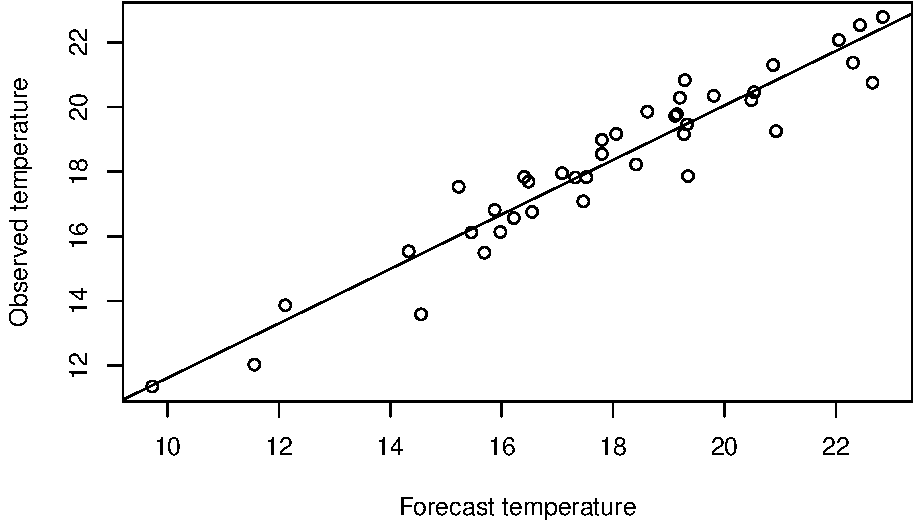
\includegraphics{graphics/unnamed-chunk-6-1.pdf}

\begin{Shaded}
\begin{Highlighting}[]
\FunctionTok{plot}\NormalTok{(x,y)}
\end{Highlighting}
\end{Shaded}

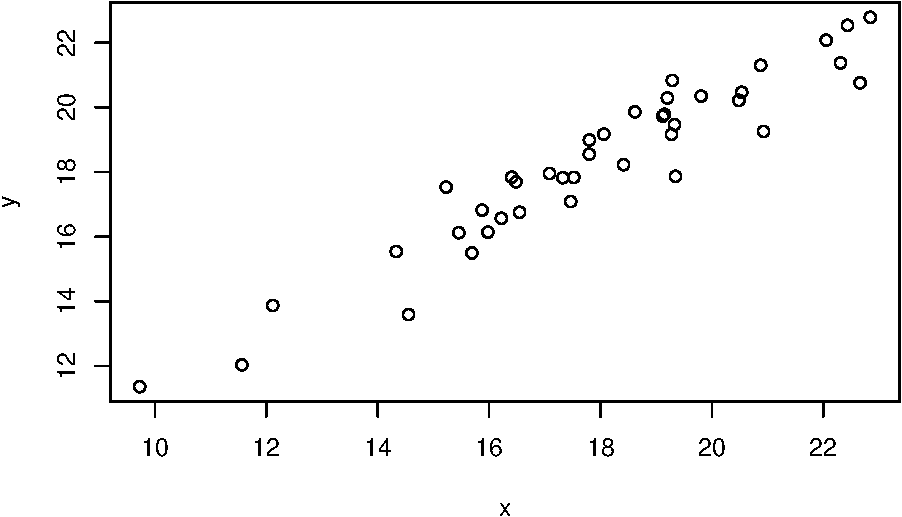
\includegraphics{graphics/unnamed-chunk-7-1.pdf}

\hypertarget{use-your-calibrated-model-to-address-your-original-question}{%
\section{Use your calibrated model to address your original question}\label{use-your-calibrated-model-to-address-your-original-question}}

\begin{Shaded}
\begin{Highlighting}[]
\NormalTok{sim\_y }\OtherTok{\textless{}{-}} \FunctionTok{rnorm}\NormalTok{(}\DecValTok{10000}\NormalTok{, theta\_hat, sigma\_hat)}

\FunctionTok{hist}\NormalTok{(sim\_y, }\AttributeTok{breaks =} \DecValTok{100}\NormalTok{)}
\end{Highlighting}
\end{Shaded}

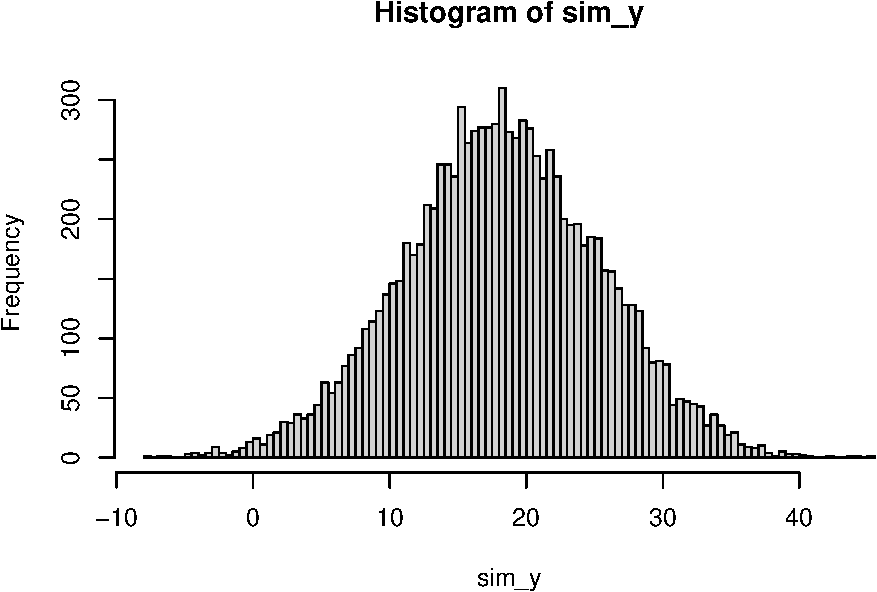
\includegraphics{graphics/generate distribution of temp based on model results-1.pdf}

\hypertarget{assignment-write-a-concept-note}{%
\chapter{Assignment: Write a concept note}\label{assignment-write-a-concept-note}}

Write a concept note for a potential time series analysis project.

\hypertarget{assignment-instructions}{%
\section{Assignment Instructions}\label{assignment-instructions}}

In just a few paragraphs (1 page max), describe an application of time series analysis that you might undertake in connection with your own research, your professional practice, or for a class project.

\hypertarget{submission-procedure}{%
\section{Submission procedure}\label{submission-procedure}}

Prepare your note in R Markdown within R Studio. Use \texttt{knitr} to generate a PDF output.

Commit your saved .Rmd and .pdf files to your (local) repo, then push your changes to your repo on the course site on Github.

When all is ready, submit your assignment on Collab. But don't attach your pdf file. Instead, a link to your .pdf file on Github.

Generate your output as a PDF rather than as HTML: Github makes is complicated to download and view .html files.

\hypertarget{choosing-a-topic}{%
\section{Choosing a topic}\label{choosing-a-topic}}

Your topic might depend on which type of degree program you are in, and how far along you are in that program.

If you are well along in a research-oriented graduate degree program, then you likely have already a fairly clear notion of the research question(s) you are addressing or plan to address, and the methods you will use to approach your question. Ideally, you will have already secured access to a time series data set that you hope to analyze. In this case, please describe the data set, and the type of useful information you hope to learn about it. If applicable, describe how this analysis could inform your research program.

If you at the beginning stages of a research-oriented degree program, you likely have some idea of the topics and methods you will use, but may not have much idea of what data sets you will use or what insights you hope to extract from those data. In this case, please think about what kinds of time series data analysis might help advance your work. It is likely that a consultation with your research advisor will be helpful. Write about your research question(s), and how analysis of time series data might help your research program. Ideally, please try to identify a data set that you could use, and describe how you can access these data.

If you are not in a research-oriented degree program, think about how a time series analysis could be applied to some aspect of your work, professional practice, or personal or career interests.

If you don't have any ideas at all, and are looking for help finding one, let me know. We will identify together a project idea and data set you can work with, possibly related to energy. But try first to think of one on your own, one that you care about.

\hypertarget{part-set-up}{%
\part{Set up}\label{part-set-up}}

\hypertarget{project-set-up-good-practices}{%
\chapter{Project set up: Good practices}\label{project-set-up-good-practices}}

\hypertarget{reproducible-workflows}{%
\section{Reproducible workflows}\label{reproducible-workflows}}

\hypertarget{setting-up-a-new-project}{%
\section{Setting up a new project}\label{setting-up-a-new-project}}

\hypertarget{folder-structure}{%
\section{Folder structure}\label{folder-structure}}

Readings:

\href{https://jhudatascience.org/tidyversecourse/intro.html\#data-science-project-organization}{TSDS Section 1.6}

\hypertarget{naming-things}{%
\section{Naming things}\label{naming-things}}

Readings:

Jenny Bryan, \href{https://speakerdeck.com/jennybc/how-to-name-files}{naming things} slide deck, Reproducible Science Workshop, 2015.

Hadley Wickham, \href{https://style.tidyverse.org/files.html\#names}{The tidyverse style guide. Section 1: ``Files''}

\hypertarget{assignment-set-up-your-computing-environment}{%
\chapter{Assignment: Set up your computing environment}\label{assignment-set-up-your-computing-environment}}

The course relies on computing resources. Please install the software as indicated on your local machine, and familiarize yourself with the associated documentation.

Topics: R, R Studio, git, Github, Markdown, R Markdown, Tidyverse and tidyverts packages for R

Assignment: Follow instructions in the course \href{https://github.com/uva-eng-time-series-sp21/sys5581-course-materials/blob/master/computing_setup_guide.pdf}{Computing setup guide}.

\hypertarget{the-r-programming-language-and-related-resources}{%
\section{The R programming language, and related resources}\label{the-r-programming-language-and-related-resources}}

We will do our coding in R, a programming language especially well-suited to statistical computing.

\begin{itemize}
\tightlist
\item
  \href{https://cran.rstudio.com/}{Download and install R}, v. 3.0.1+.

  \begin{itemize}
  \tightlist
  \item
    Note: There is a later version, v. 4.0.2, in development, but you shouldn't need it.
  \end{itemize}
\end{itemize}

\href{https://rstudio.com/products/rstudio/}{R Studio} is an integrated development environment (IDE) for R. It offers a variety of utilities to enhance the experience of coding and generating documents.

\begin{itemize}
\tightlist
\item
  \href{https://rstudio.com/products/rstudio/download/\#download}{Download and install R Studio}, v. 1.4.1+.
\end{itemize}

\href{https://www.tidyverse.org/}{Tidyverse} is a collection of packages that extend the capabilities of R for doing data science.

\begin{itemize}
\tightlist
\item
  Install the Tidyverse packages for R: From the Console tab in R Studio (or from R running in a Terminal window), enter:
\end{itemize}

\begin{Shaded}
\begin{Highlighting}[]
\FunctionTok{install.packages}\NormalTok{(}\StringTok{"tidyverse"}\NormalTok{)}
\end{Highlighting}
\end{Shaded}

\begin{itemize}
\item
  Alternatively, you may install packages via the \texttt{Packages} tab in R Studio.
\item
  Optional: To learn how to wrangle and visualize data using the Tidyverse packages, you may find it useful to go through the \href{https://learn.datacamp.com/skill-tracks/tidyverse-fundamentals}{Tidyverse Fundamentals with R} modules on \href{https://learn.datacamp.com/}{Datacamp}.

  \begin{itemize}
  \tightlist
  \item
    Datacamp also offers \href{https://learn.datacamp.com/career-tracks/data-scientist-with-r}{a range of other learning modules for developing data science skills in R}.
  \end{itemize}
\end{itemize}

\href{https://tidyverts.org/}{Tidyverts} is a collection of R packages for time series analysis designed to work well with the Tidyverse packages. Each package in the tidyverts suite needs to be installed individually:

\begin{itemize}
\tightlist
\item
  From the Console tab in R Studio (or from R running in a Terminal window), enter:
\end{itemize}

\begin{Shaded}
\begin{Highlighting}[]
\FunctionTok{install.packages}\NormalTok{(}\FunctionTok{c}\NormalTok{(}\StringTok{"tsibble"}\NormalTok{, }\StringTok{"tsibbledata"}\NormalTok{, }\StringTok{"feasts"}\NormalTok{, }\StringTok{"fable"}\NormalTok{))}
\end{Highlighting}
\end{Shaded}

\begin{itemize}
\tightlist
\item
  You don't need to install the \texttt{tsibbletalk} and \texttt{fable.prophet} packages; we probably won't use them in this course.
\end{itemize}

\hypertarget{git-and-github}{%
\section{Git and Github}\label{git-and-github}}

Reference: \href{https://happygitwithr.com/}{Happy Git and GitHub for the useR}

\href{https://git-scm.com/}{Git} is software for version control. Github is a web service that provides remote storage and access to files via git. This setup greatly facilitates collaboration between multiple individuals working on the same code base.

First watch this short YouTube video to get an orientation to git and Github: \href{https://www.youtube.com/watch?v=l2ftm-YwJs8}{Git and GitHub for an Organized Project (STAT 545 Episode 2-A)} from the University of British Columbia.

Then install git on your machine and link it to your R Studio instance and your file repository on Github:

\begin{itemize}
\tightlist
\item
  \href{https://jennybc.github.io/2014-05-12-ubc/ubc-r/session03_git.html}{Follow these instructions} to \href{https://git-scm.com/downloads}{download and install git} and to link git with R Studio.
\end{itemize}

A collection of files associated with a single project is in git-speak called a ``repository'' or \emph{``repo''}. You should already have a basic repo set up for you on the course site on Github. The next step is to copy (``clone'') this remote repo to your local machine.

\begin{itemize}
\tightlist
\item
  Clone your course repo on Github to a new R Studio project on your local machine.

  \begin{itemize}
  \tightlist
  \item
    Navigate to \href{https://github.com/uva-eng-time-series-sp21}{the course website on Github}. Select your repo.
  \item
    Click on the green button labeled ``Code''. Copy the URL.
  \item
    In the R Studio window, from the pull-down menu in the upper-right corner, select \texttt{New\ Project...}, \texttt{Version\ Control}, \texttt{Git}. Paste the URL into the dialog box labeled \texttt{Repository\ URL}.
  \item
    Optional: Change the name of the project folder, and the location of this folder on your local directory tree.
  \item
    Click on \texttt{Create\ Project}. The files from your remote repo should be copied to your local machine in a new folder with the name you chose.
  \end{itemize}
\item
  Optional: \href{https://git-scm.com/downloads/guis}{Download and install the Github desktop client}, or an alternative GUI client.

  \begin{itemize}
  \tightlist
  \item
    The git operations you need for this course can be managed within R Studio, from the \texttt{Git} tab. Some more advanced operations require using either a Terminal window, or a Git desktop client.
  \end{itemize}
\end{itemize}

As you get going, you will likely want to learn more about how to work with git and Github. \href{https://git-scm.com/}{Review the documentation for git} and \href{https://guides.github.com/introduction/flow/}{this Github Guide}. Learn the basics.

\hypertarget{using-personal-tokens-to-access-github}{%
\subsection{Using personal tokens to access Github}\label{using-personal-tokens-to-access-github}}

Github is phasing out the use of passwords for authorizations.

\begin{verbatim}
---- Forwarded Message -----
From: GitHub <noreply@github.com>
To: Arthur Small <asmall@virginia.edu>
Sent: Sunday, February 21, 2021, 6:20:58 AM EST
Subject: [GitHub] Deprecation Notice

Hi @arthursmalliii,

You recently used a password to access the repository at uva-eng-time-series-sp21/coronato-nicholas with git using git/2.30.0.

Basic authentication using a password to Git is deprecated and will soon no longer work. Visit https://github.blog/2020-12-15-token-authentication-requirements-for-git-operations/ for more information around suggested workarounds and removal dates.

Thanks,
The GitHub Team
\end{verbatim}

Instead, you must create a personal access token. See the Github documentation.

\hypertarget{markdown-and-r-markdown}{%
\section{Markdown and R Markdown}\label{markdown-and-r-markdown}}

Markdown is a markup language: a set of formatting instructions for rendering documents. R Markdown is an extension of Markdown that allows for embedding chunks of R code into a Markdown document. In this course, we will write our work in R Markdown within the R Studio environment, then use the \texttt{knitr} package to generate HTML and PDF output files.

For a nice introduction to Markdown and R Markdown, watch the short YouTube video \href{https://www.youtube.com/watch?v=ZzDSkBgt9xQ}{Reproducible Reports with R Markdown (STAT 545 Episode 3-A)} from the University of British Columbia.

As you proceed in creating your documents, you will probably want to access additional resources:

\begin{itemize}
\item
  From within R Studio, you can access an R Markdown Cheat Sheet via \texttt{Help/Cheatsheets}.
\item
  Markdown reference: \url{https://www.markdownguide.org/}
\item
  R Markdown reference: \url{https://rmarkdown.rstudio.com/}
\end{itemize}

\hypertarget{bibliographic-resources-zotero-and-bibtex}{%
\section{Bibliographic resources: Zotero and Bibtex}\label{bibliographic-resources-zotero-and-bibtex}}

{[}Coming soon\ldots{]}

\hypertarget{general-course-web-resources}{%
\section{General course web resources}\label{general-course-web-resources}}

\begin{itemize}
\tightlist
\item
  \href{https://collab.its.virginia.edu}{Collab class site}, for basic course information, assignments, office hours sign-up, links to online textbook and other resources.
\item
  \href{https://github.com/uva-eng-time-series-sp21}{Github class site}, for posting and sharing code.
\item
  Zoom, for class sessions, recordings, and office hours.
\end{itemize}

\hypertarget{part-data-acquisition-and-preparation}{%
\part{Data Acquisition and Preparation}\label{part-data-acquisition-and-preparation}}

\hypertarget{finding-a-dataset-for-your-project}{%
\chapter{Finding a dataset for your project}\label{finding-a-dataset-for-your-project}}

\begin{figure}

{\centering \includegraphics[width=1\linewidth]{graphics/ff_311_newyork1b_f} 

}

\caption{New York City 311 calls by time of day, September 8--15, 2010. Source: [Wired Magazine](https://www.wired.com/2010/11/ff_311_new_york/)}\label{fig:unnamed-chunk-10}
\end{figure}

Readings:

\href{https://jhudatascience.org/tidyversecourse/model.html\#data-needs}{TSDS, Section 5.4}

\hypertarget{appropriate-data-sets-for-time-series-analysis}{%
\section{Appropriate data sets for time series analysis}\label{appropriate-data-sets-for-time-series-analysis}}

Just because your data set has some dates and times in it, doesn't mean it is appropriate for a time series analysis.

Time series methods are generally appropriate when data are measured at regular intervals, over a fairly long period.

\hypertarget{data-resources}{%
\section{Data resources}\label{data-resources}}

The UVA Libraries offer excellent \href{https://www.library.virginia.edu/services}{data services}, including resources for \href{https://data.library.virginia.edu/datasources/}{data discovery and access}. If you haven't settled on your own dataset to analyze for your project, you may find one by browsing their \href{https://data.library.virginia.edu/datasources/find-data/}{recommended top data sources} and \href{https://data.library.virginia.edu/datasources/licensed/}{licensed data}. If you need personal assistance, you are invited to contact UVA's Data Librarian, Jenn Huck, at \href{mailto:data@virginia.edu}{\nolinkurl{data@virginia.edu}} to schedule an appointment.

Some data sources you might check out:

\begin{itemize}
\tightlist
\item
  The \href{https://data.library.virginia.edu/datasources/licensed/cnts/}{Cross-National Time-Series Data Archive} provides more than 200 years of annual data from 1815 onward for over 200 countries. It consists of 196 data variables used by academia, government, finance and media.
\item
  \href{https://www.eia.gov/tools/}{U.S. Energy Information Administration}. Diverse datasets on energy.
\item
  ``\href{https://github.com/awesomedata/awesome-public-datasets}{Awesome Public Datasets}''.
\item
  \href{https://flowingdata.com/category/statistics/data-sources/}{Flowing Data} data sources.
\item
  \href{https://openpolicing.stanford.edu/}{The Stanford Open Policing Project}. ``On a typical day in the United States, police officers make more than 50,000 traffic stops. Our team is gathering, analyzing, and releasing records from millions of traffic stops by law enforcement agencies across the country.''
\item
  \href{https://www.data.gov/opendata/}{Open U.S. Federal Government Data}.
\item
  \href{https://opendata.charlottesville.org/}{Charlottesville, Virginia open data}
\item
  \href{https://portal.311.nyc.gov/article/?kanumber=KA-02893}{New York City 311 Data}.
\end{itemize}

\hypertarget{data-acquisition-and-extraction}{%
\chapter{Data acquisition and extraction}\label{data-acquisition-and-extraction}}

Readings:

\href{https://jhudatascience.org/tidyversecourse/get-data.html}{TSDS, Chapter 2}

\hypertarget{access-protocols-and-permissions}{%
\section{Access protocols and permissions}\label{access-protocols-and-permissions}}

\begin{itemize}
\item
  Reproducible extraction of data from source location: may be complicated by access protocols.

  \begin{itemize}
  \tightlist
  \item
    access tokens; APIs
  \item
    raw data from github for private repos
  \item
    databases
  \item
    package \texttt{httr} to access data from websites
  \end{itemize}
\end{itemize}

\hypertarget{accessing-databases}{%
\section{Accessing databases}\label{accessing-databases}}

\begin{Shaded}
\begin{Highlighting}[]
\NormalTok{esales }\OtherTok{\textless{}{-}} \FunctionTok{dbGetQuery}\NormalTok{(db,}\StringTok{\textquotesingle{}SELECT * from eia\_elec\_sales\_va\_all\_m\textquotesingle{}}\NormalTok{) }\CommentTok{\# SQL code to retrieve data from a table in the remote database}
\CommentTok{\# str(esales)}
\NormalTok{esales }\OtherTok{\textless{}{-}} \FunctionTok{as\_tibble}\NormalTok{(esales) }\CommentTok{\# Convert dataframe to a \textquotesingle{}tibble\textquotesingle{} for tidyverse work}
\CommentTok{\# str(esales)}
\end{Highlighting}
\end{Shaded}

\begin{Shaded}
\begin{Highlighting}[]
\CommentTok{\# Reference: https://arrow.apache.org/docs/r/}
\CommentTok{\# if(!(\textquotesingle{}arrow\textquotesingle{} \%in\% installed.packages())) install.packages(\textquotesingle{}arrow\textquotesingle{})}
\FunctionTok{library}\NormalTok{(arrow)}
\FunctionTok{write\_feather}\NormalTok{(esales, }\StringTok{"esales.feather"}\NormalTok{)}
\end{Highlighting}
\end{Shaded}

\begin{Shaded}
\begin{Highlighting}[]
\CommentTok{\# Close connection {-}{-} this is good practice}
\FunctionTok{dbDisconnect}\NormalTok{(db)}
\FunctionTok{dbUnloadDriver}\NormalTok{(db\_driver)}
\end{Highlighting}
\end{Shaded}

\hypertarget{other-comments}{%
\section{Other comments}\label{other-comments}}

Make your extraction code ``as reproducible as possible'', subject to these access constraints. At minimum, document clearly how you obtained the data, so others could follow your path, even if not via pure code.

Keep your raw data in read-only mode. Don't edit these files.

Write code to transform the raw data into form you will use for analysis. Don't do it manually.

\hypertarget{assignment-update-your-concept-and-get-your-data}{%
\chapter{Assignment: Update your concept and get your data}\label{assignment-update-your-concept-and-get-your-data}}

\hypertarget{refine-your-concept-note}{%
\section{Refine your concept note}\label{refine-your-concept-note}}

\begin{itemize}
\tightlist
\item
  State clearly the question(s) you will attempt to answer.
\item
  Make sure this is a clear, answerable question. Don't do ``a study of\ldots{}''.
\item
  Make sure this is genuinely a question about a \emph{time series process}.

  \begin{itemize}
  \tightlist
  \item
    Imagine a metronome: each time you hear a `click', another row of data values gets added to your table.
  \end{itemize}
\end{itemize}

\hypertarget{identify-a-time-series-data-set-you-want-to-work-with}{%
\section{Identify a time series data set you want to work with}\label{identify-a-time-series-data-set-you-want-to-work-with}}

Ideally, identify a data set that you that you might use as the basis for your class project. You need not necessarily commit at this time to using this data set for your project. However, bear in mind that you will in this assignment be investing time and effort in acquiring, cleaning, and organizing the data set. It is better for you if you invest that effort on the data set you will later analyze.

Please do not use a data set that already come packaged with \texttt{R} or that is otherwise already cleaned up. The point of this assignment is to learn how to use tools from the Tidyverse and tidyverts packages when working with data you acquire ``in the wild''.

\hypertarget{acquire-the-data-from-its-source-location-reproducibly}{%
\section{Acquire the data from its source location, reproducibly}\label{acquire-the-data-from-its-source-location-reproducibly}}

You typically will need first to \emph{extract} your data from its original source (e.g., an Excel file, an API, a database, a cloud hosting service).

\hypertarget{stage-your-raw-data}{%
\section{Stage your raw data}\label{stage-your-raw-data}}

If your data files are smaller than 25 MB, you may synch them to Github with the rest of your repo. Put them in the \texttt{raw\_data} folder.

Files larger than 25 MB should not be posted to Github. Instead, post them to a cloud storage service such as Google Drive, One Drive, Box, or Dropbox. Your code should include a reproducible procedure for downloading the data in these files to a local drive.

\hypertarget{submission-procedure-1}{%
\section{Submission procedure}\label{submission-procedure-1}}

Create a new R Markdown document for this work, inside R Studio. Code and document all these steps in a single .Rmd file.

To submit your work: knit your .Rmd file to generate a .pdf file. Push both the .Rmd and .pdf files to your Repo on Github, along with any supporting files. Submit your assignment on Collab, enclosing a link to your .pdf file on Github.

\hypertarget{other-comments-1}{%
\section{Other comments}\label{other-comments-1}}

All steps should be fully \emph{reproducible}. This means: If I, or anyone, rerun the code in your R Markdown file and reknit the .Rmd file to generate a new PDF output, I should be able to execute all your computational steps and regenerate your PDF essentially exactly.

\hypertarget{data-preparation-strategy}{%
\chapter{Data preparation strategy}\label{data-preparation-strategy}}

Topics:

\begin{itemize}
\tightlist
\item
  Tidy data
\item
  \texttt{tsibble} objects for storing, manipulating, and visualizing time series data. Frequency of time series: the \texttt{index} parameter. \texttt{key} parameter(s).
\item
  Applying \texttt{dplyr} verbs to \texttt{tsibble} objects: \texttt{filter}, \texttt{select}, \texttt{mutate}, \texttt{group\_by}, \texttt{summarize}
\end{itemize}

Readings:

\begin{itemize}
\tightlist
\item
  \href{https://jhudatascience.org/tidyversecourse/wrangle-data.html\#anonymous-functions}{TSDS, Sections 3.1-3.9}
\item
  FPP3, Section 2.1
\end{itemize}

Optional: To learn how to wrangle and visualize data using the Tidyverse packages, you may find it useful to go through the \href{https://learn.datacamp.com/skill-tracks/tidyverse-fundamentals}{Tidyverse Fundamentals with R} modules on \href{https://learn.datacamp.com/}{Datacamp}. Datacamp also offers \href{https://learn.datacamp.com/career-tracks/data-scientist-with-r}{a range of other learning modules for developing data science skills in R}.

Assignment: \href{https://github.com/uva-eng-time-series-sp21/sys5581-course-materials/blob/master/assignments/assignment_data_etl.pdf}{Extract and prepare your data}.

\hypertarget{overview-extraction-transformation-and-loading-of-data}{%
\section{Overview: Extraction, transformation, and loading of data}\label{overview-extraction-transformation-and-loading-of-data}}

Before undertaking any data analysis project, you need to organize your data into a format to make it ready for analysis. Very commonly, the data you wish to work with will not come to you in a nice format that makes it ready to analyze. Often it will be necessary to transform the data, applying a sequence of manipulations to get it into a nice format such as a single table.

If you have saved your prepared table to a database or local file, your may finally need to load the data into memory on your working machine as a prelude to commence analysis. These steps together are the \emph{extract-transform-load} (ETL) stage of a data analysis project.

The bad news is that working data scientists generally report that the ETL stage is the most time-consuming part of a data science project. The good news is that the \texttt{R} \texttt{tidyverse} packages offer a number of helpful tools to somewhat ease the pain of ETL work, also known informally as \emph{data wrangling}.\footnote{``Wrangling'' refers to work with cattle, sheep, and other livestock.}

The ETL steps needed for a given project will depend on the nature of the data and on how they are originally organized. We can characterize how we want the data to look at the end of the ETL stage. To the extent possible, we want the data to be \emph{tidy}.

\hypertarget{organize-your-data-into-a-tidy-data-frame}{%
\section{\texorpdfstring{Organize your data into a \emph{tidy} data frame}{Organize your data into a tidy data frame}}\label{organize-your-data-into-a-tidy-data-frame}}

Readings: \href{https://jhudatascience.org/tidyversecourse/intro.html\#tidy-data}{TSDS Sections 1.2-1.3}

Hadley Wickham \citeyearpar{wickhamTidyData2014} codifies the concept of \href{https://cran.r-project.org/web/packages/tidyr/vignettes/tidy-data.html}{tidy data}:

\begin{quote}
Tidy data is a standard way of mapping the meaning of a dataset to its structure. A dataset is messy or tidy depending on how rows, columns and tables are matched up with observations, variables and types. In tidy data:
\end{quote}

\begin{quote}
\begin{enumerate}
\def\labelenumi{\arabic{enumi}.}
\tightlist
\item
  Each variable forms a column.
\item
  Each observation forms a row.
\item
  Each type of observational unit forms a table.
\end{enumerate}
\end{quote}

``Real datasets can, and often do, violate the three precepts of tidy data in almost every way imaginable. While occasionally you do get a dataset that you can start analysing immediately, this is the exception, not the rule.'' In real life, the systems people and organizations use to collect, manage, and store data are governed by many priorities: end-user convenience, clarity of presentation, storage costs, processing speed, etc. Making data fit for analysis by data scientists is typically a minor consideration, if it is thought of at all.

Expanding on the theme, Wickham identifies five of the most common problems with non-tidy, ``messy'' datasets:

\begin{quote}
\begin{itemize}
\tightlist
\item
  Column headers are values, not variable names.
\item
  Multiple variables are stored in one column.
\item
  Variables are stored in both rows and columns.
\item
  Multiple types of observational units are stored in the same table.
\item
  A single observational unit is stored in multiple tables.
\end{itemize}
\end{quote}

The Tidyverse packages integrate a range of tools to help with transforming the messy data often encountered in the wild into tidy formats more suitable for analysis. See the \href{https://www.tidyverse.org/}{Tidyverse website} for an overview, or \href{https://www.coursera.org/specializations/tidyverse-data-science-r}{this Coursera course} for more guidance.

\begin{itemize}
\tightlist
\item
  Organize your data table(s) so that they `match' your question.
\end{itemize}

\hypertarget{convert-your-data-into-a-tsibble-object}{%
\section{\texorpdfstring{Convert your data into a \texttt{tsibble} object}{Convert your data into a tsibble object}}\label{convert-your-data-into-a-tsibble-object}}

In this step of the assignment, you will convert your tidy data frame into a \texttt{tsibble} object. Doing so in effect tells \texttt{R}: ``These data actually form a time series. One column, which I designate the \texttt{index}, contains time values, in equal intervals.'' Taking this step enables the use of specific tools for data visualization, exploratory analysis, and forecasting for time series data. The \href{https://tsibble.tidyverts.org/}{tsibble package} for R provides ``a data infrastructure for tidy temporal data''. Review the documentation for instructions.

\hypertarget{data-preparation-strategy-design-your-end-point-data-tables}{%
\section{Data preparation strategy: Design your end-point data table(s)}\label{data-preparation-strategy-design-your-end-point-data-tables}}

Starting point: Multiple source files, mess, etc. This is real life as a data scientist.

What's your desired end point? How will you prepare your data to make it ready to analyze?

Data preparation is a creative activity. (Your jobs are secure.)

\hypertarget{design-your-end-point-first-at-least-in-your-head.}{%
\subsection{Design your end point first (at least, in your head).}\label{design-your-end-point-first-at-least-in-your-head.}}

\begin{itemize}
\tightlist
\item
  Which columns? In which order?
\item
  Which data types should the different columns have?
\item
  For \texttt{tsibble} objects:

  \begin{itemize}
  \tightlist
  \item
    Which column is the \texttt{index}? Must have date+time values, at regular intervals.
  \item
    Which columns contain \texttt{key} values?

    \begin{itemize}
    \tightlist
    \item
      These are values that \emph{don't} change with time.
    \item
      Each value of the \texttt{key} corresponds to a distinct time series.
    \item
      Cannot have duplicate rows that share an \texttt{index} + \texttt{key} value.
    \end{itemize}
  \item
    Remaining columns contain observational data: one row for each time step and \texttt{key} value.

    \begin{itemize}
    \tightlist
    \item
      What data types should these be?
    \item
      Might choose to drop columns you aren't going to use, to reduce clutter.
    \end{itemize}
  \end{itemize}
\end{itemize}

\hypertarget{ts-table}{%
\subsection{Typical structure for a time series data table}\label{ts-table}}

\begin{longtable}[]{@{}ccccc@{}}
\toprule
Date + time & Series & Value\_1 & Value\_2 & Value\_3 \\
\midrule
\endhead
2020-02-01 & ``Virginia'' & 33.57 & 29 & ``friendly'' \\
2020-02-01 & ``Idaho'' & 0.22 & 18 & ``hostile'' \\
\ldots{} & \ldots{} & \ldots{} & \ldots{} & \ldots{} \\
\texttt{index} & \texttt{key} & & & \\
{[}date{]} & {[}fctr{]} & {[}dbl{]} & {[}int{]} & {[}fctr{]} \\
\bottomrule
\end{longtable}

Then wrangle your data to get to your desired end point.

Recommended practices:

\begin{itemize}
\tightlist
\item
  Put \texttt{index} field in the left-most column.
\item
  Next, put all the \texttt{key} fields.
\item
  Then finally the data values. Start with the most important ones.
\end{itemize}

\hypertarget{additional-resources-and-next-steps}{%
\section{Additional resources and next steps}\label{additional-resources-and-next-steps}}

To learn how to wrangle and visualize data using the Tidyverse packages, you may find it useful to go through the \href{https://learn.datacamp.com/skill-tracks/tidyverse-fundamentals}{Tidyverse Fundamentals with R} modules on \href{https://learn.datacamp.com/}{Datacamp}, or \href{https://www.coursera.org/specializations/tidyverse-data-science-r}{the analogous course on Coursera}. Datacamp also offers \href{https://learn.datacamp.com/career-tracks/data-scientist-with-r}{a range of other learning modules for developing data science skills in R}.

With your data organized into a \texttt{tsibble} object, you are positioned to do some \emph{exploratory data analysis}, the topic of the next assignment. If you want to get a head start, check out the functions for data visualization and exploratory analysis of time series in the \href{https://feasts.tidyverts.org/}{feasts package}. Or work through the examples in \href{https://otexts.com/fpp3/graphics.html}{Chapter 2} or \href{https://otexts.com/fpp3/features.html}{Chapter 4} of \href{https://otexts.com/fpp3/}{Forecasting: Principles and Practice, 3rd ed.}

\hypertarget{reading-in-data-from-source-files}{%
\chapter{Reading in data from source files}\label{reading-in-data-from-source-files}}

\hypertarget{first-examine-text-files-in-a-text-editor}{%
\section{First, examine text files in a text editor}\label{first-examine-text-files-in-a-text-editor}}

It's generally a good idea to examine the contents of an unfamiliar text data file visually, in text editor, before starting to work on it. You can open smaller files inside RStudio. For files too big to open inside RStudio, you can use a dedicated text editor like \href{https://atom.io/}{Atom}.

This code prints out the first ten lines of the text file ``PetroStocks.csv''.

\begin{Shaded}
\begin{Highlighting}[]
\CommentTok{\# Print out first ten rows of file "data/PetroStocks.csv"}
\FunctionTok{readLines}\NormalTok{(}\StringTok{"data/PetroStocks.csv"}\NormalTok{, }\AttributeTok{n=}\DecValTok{10}\NormalTok{) }\SpecialCharTok{\%\textgreater{}\%} \FunctionTok{paste0}\NormalTok{(}\AttributeTok{collapse=}\StringTok{"}\SpecialCharTok{\textbackslash{}n}\StringTok{"}\NormalTok{) }\SpecialCharTok{\%\textgreater{}\%}\NormalTok{ cat}
\end{Highlighting}
\end{Shaded}

\begin{verbatim}
## Back to Contents,Data 1: Petroleum Stocks,,,,,,,,,,,,,,,,,,,
## Sourcekey,WCRSTUS1,WCESTUS1,WCSSTUS1,WGTSTUS1,WGRSTUS1,WG4ST_NUS_1,WBCSTUS1,W_EPOOXE_SAE_NUS_MBBL,WKJSTUS1,WDISTUS1,WD0ST_NUS_1,WD1ST_NUS_1,WDGSTUS1,WRESTUS1,WPRSTUS1,W_EPPO6_SAE_NUS_MBBL,WUOSTUS1,WTTSTUS1,WTESTUS1,
## Date,Weekly U.S. Ending Stocks of Crude Oil  (Thousand Barrels),Weekly U.S. Ending Stocks excluding SPR of Crude Oil  (Thousand Barrels),Weekly U.S. Ending Stocks of Crude Oil in SPR  (Thousand Barrels),Weekly U.S. Ending Stocks of Total Gasoline  (Thousand Barrels),Weekly U.S. Ending Stocks of Reformulated Motor Gasoline  (Thousand Barrels),Weekly U.S. Ending Stocks of Conventional Motor Gasoline  (Thousand Barrels),Weekly U.S. Ending Stocks of Gasoline Blending Components  (Thousand Barrels),Weekly U.S. Ending Stocks of Fuel Ethanol  (Thousand Barrels),Weekly U.S. Ending Stocks of Kerosene-Type Jet Fuel  (Thousand Barrels),Weekly U.S. Ending Stocks of Distillate Fuel Oil  (Thousand Barrels),"Weekly U.S. Ending Stocks of Distillate Fuel Oil, 0 to 15 ppm Sulfur  (Thousand Barrels)","Weekly U.S. Ending Stocks of Distillate Fuel Oil, Greater than 15 to 500 ppm Sulfur  (Thousand Barrels)","Weekly U.S. Ending Stocks of Distillate Fuel Oil, Greater Than 500 ppm Sulfur  (Thousand Barrels)",Weekly U.S. Ending Stocks of Residual Fuel Oil  (Thousand Barrels),Weekly U.S. Propane and Propylene Ending Stocks Excluding Propylene at Terminal (Thousand Barrels),Weekly U.S. Ending Stocks of Other Oils (Excluding Fuel Ethanol)  (Thousand Barrels),Weekly U.S. Ending Stocks of Unfinished Oils  (Thousand Barrels),Weekly U.S. Ending Stocks of Crude Oil and Petroleum Products  (Thousand Barrels),Weekly U.S. Ending Stocks excluding SPR of Crude Oil and Petroleum Products  (Thousand Barrels),
## "Aug 20, 1982",609219,338764,270455,,,,,,33523,149415,,,,51168,,,119293,,,
## "Aug 27, 1982",608741,336138,272603,,,,,,33897,154589,,,,48544,,,119863,,,
## "Sep 24, 1982",612419,335586,276833,,,,,,34949,158684,,,,57813,,,117686,,,
## "Oct 01, 1982",612419,334786,277633,,,,,,33919,154461,,,,60828,,,118759,,,
## "Oct 08, 1982",613985,335260,278725,,,,,,32347,158242,,,,60381,,,119017,,,
## "Oct 15, 1982",607781,326979,280802,,,,,,33382,161578,,,,60929,,,117603,,,
## "Oct 22, 1982",617763,334370,283393,,,,,,34280,162934,,,,61688,,,115236,,,
\end{verbatim}

What do you see?

\hypertarget{read-in-csv-files}{%
\section{Read in CSV files}\label{read-in-csv-files}}

Using \texttt{read\_csv()}: Example:

\begin{Shaded}
\begin{Highlighting}[]
\CommentTok{\# Data Source: https://www.eia.gov/petroleum/supply/weekly/}
\FunctionTok{library}\NormalTok{(readr)}

\CommentTok{\# Original code:}
\NormalTok{PetroStocksData }\OtherTok{\textless{}{-}}\NormalTok{ readr}\SpecialCharTok{::}\FunctionTok{read\_csv}\NormalTok{(}\StringTok{"data/PetroStocks.csv"}\NormalTok{)}
\FunctionTok{names}\NormalTok{(PetroStocksData) }\OtherTok{\textless{}{-}}\NormalTok{ PetroStocksData[}\DecValTok{2}\NormalTok{,] }\CommentTok{\# assign names to columns}
\NormalTok{PetroStocksData }\OtherTok{\textless{}{-}}\NormalTok{ PetroStocksData[}\SpecialCharTok{{-}}\DecValTok{1}\NormalTok{,]       }\CommentTok{\# remove first unused row}
\NormalTok{PetroStocksData }\OtherTok{\textless{}{-}}\NormalTok{ PetroStocksData[}\SpecialCharTok{{-}}\DecValTok{1}\NormalTok{,]       }\CommentTok{\# remove another unused row}
\end{Highlighting}
\end{Shaded}

\hypertarget{declaring-data-types}{%
\subsection{Declaring data types}\label{declaring-data-types}}

Declaring data types as you read in data.

Choose your data types!

Reference: R4DS Ch. 15, 16

\begin{Shaded}
\begin{Highlighting}[]
\DocumentationTok{\#\#\# Revised using readr::read\_csv() to skip empty rows and declare data types}
\DocumentationTok{\#\#\# Declare column types within the read\_csv() function call, to save yourself trouble later:}
\NormalTok{ps\_tbl }\OtherTok{\textless{}{-}}\NormalTok{ readr}\SpecialCharTok{::}\FunctionTok{read\_csv}\NormalTok{(}\StringTok{"data/PetroStocks.csv"}\NormalTok{, }\AttributeTok{skip =} \DecValTok{2}\NormalTok{, }\AttributeTok{col\_types =} \FunctionTok{cols}\NormalTok{(}\AttributeTok{.default =} \FunctionTok{col\_double}\NormalTok{(),}
                                                                       \StringTok{"Date"}   \OtherTok{=} \FunctionTok{col\_character}\NormalTok{())) }

\DocumentationTok{\#\#\# Reference: https://readr.tidyverse.org/reference/read\_delim.html}
\end{Highlighting}
\end{Shaded}

\hypertarget{data-cleaning}{%
\chapter{Data cleaning}\label{data-cleaning}}

\hypertarget{dropping-empty-rows-and-columns}{%
\section{Dropping empty rows and columns}\label{dropping-empty-rows-and-columns}}

\begin{Shaded}
\begin{Highlighting}[]
\CommentTok{\# Original: empty column identified manually}
\NormalTok{PetroStocksData }\OtherTok{\textless{}{-}}\NormalTok{ PetroStocksData[,}\SpecialCharTok{{-}}\DecValTok{21}\NormalTok{] }\CommentTok{\# Delete unused last column}

\DocumentationTok{\#\#\# Revised: This code removes *all* empty columns:}
\NormalTok{ps\_tbl }\SpecialCharTok{\%\textgreater{}\%} \FunctionTok{select\_if}\NormalTok{(}\ControlFlowTok{function}\NormalTok{(x) }\SpecialCharTok{!}\FunctionTok{all}\NormalTok{(}\FunctionTok{is.na}\NormalTok{(x))) }\OtherTok{{-}\textgreater{}}\NormalTok{ ps\_tbl}
\end{Highlighting}
\end{Shaded}

\begin{Shaded}
\begin{Highlighting}[]
\CommentTok{\# Original: empty row identified manually:}
\NormalTok{PetroStocksData }\OtherTok{\textless{}{-}}\NormalTok{ PetroStocksData[}\SpecialCharTok{{-}}\DecValTok{2004}\NormalTok{,] }\CommentTok{\# Delete unused last row}

\DocumentationTok{\#\#\# Revised: This code removes all empty rows:}
\NormalTok{ps\_tbl }\SpecialCharTok{\%\textgreater{}\%} \FunctionTok{filter}\NormalTok{(}\SpecialCharTok{!}\FunctionTok{across}\NormalTok{(}\FunctionTok{everything}\NormalTok{(), is.na)) }\OtherTok{{-}\textgreater{}}\NormalTok{ ps\_tbl}
\end{Highlighting}
\end{Shaded}

\hypertarget{transform-a-data-frame-to-tsibble-object}{%
\chapter{\texorpdfstring{Transform a data frame to \texttt{tsibble} object}{Transform a data frame to tsibble object}}\label{transform-a-data-frame-to-tsibble-object}}

Readings: FPP3, Section 2.1

Convert the data frame into a time series \texttt{tsibble} object.

\begin{Shaded}
\begin{Highlighting}[]
\CommentTok{\# install.packages("tsibble")}
\FunctionTok{library}\NormalTok{(tsibble) }\CommentTok{\# Reference: https://tsibble.tidyverts.org/articles/intro{-}tsibble.html}

\NormalTok{esales }\OtherTok{\textless{}{-}}\NormalTok{ arrow}\SpecialCharTok{::}\FunctionTok{read\_feather}\NormalTok{(}\StringTok{"data/esales.feather"}\NormalTok{)}
\NormalTok{esales }\SpecialCharTok{\%\textgreater{}\%}
\NormalTok{  dplyr}\SpecialCharTok{::}\FunctionTok{select}\NormalTok{(date, }\AttributeTok{sales\_GWh =}\NormalTok{ value) }\OtherTok{{-}\textgreater{}}\NormalTok{ esales\_tbl}
\NormalTok{esales\_tbl }\SpecialCharTok{\%\textgreater{}\%} \FunctionTok{as\_tsibble}\NormalTok{(}\AttributeTok{index =}\NormalTok{ date) }\OtherTok{{-}\textgreater{}}\NormalTok{ elsales\_tbl\_ts}

\FunctionTok{print}\NormalTok{(elsales\_tbl\_ts)}
\end{Highlighting}
\end{Shaded}

\begin{verbatim}
## # A tsibble: 233 x 2 [1D]
##    date       sales_GWh
##    <date>         <dbl>
##  1 2001-01-01     9576.
##  2 2001-02-01     7820.
##  3 2001-03-01     8070.
##  4 2001-04-01     7153.
##  5 2001-05-01     7224.
##  6 2001-06-01     8264.
##  7 2001-07-01     8896.
##  8 2001-08-01     9404.
##  9 2001-09-01     7753.
## 10 2001-10-01     7272.
## # ... with 223 more rows
\end{verbatim}

\hypertarget{time-indexing}{%
\section{Time indexing}\label{time-indexing}}

See R4DS ch.~16.

Depending on how dates and times are recorded in your raw data, you may face more or less work to organize them into form(s) suitable as \texttt{tsibble} index variable.

The \texttt{lubridate} and \texttt{hms} packages may be valuable.

\begin{Shaded}
\begin{Highlighting}[]
\CommentTok{\# install.packages("feasts"), Reference: https://feasts.tidyverts.org/}
\FunctionTok{library}\NormalTok{(feasts)}

\NormalTok{elsales\_tbl\_ts }\SpecialCharTok{\%\textgreater{}\%}
  \FunctionTok{mutate}\NormalTok{(}\AttributeTok{Month =}\NormalTok{ tsibble}\SpecialCharTok{::}\FunctionTok{yearmonth}\NormalTok{(date)) }\SpecialCharTok{\%\textgreater{}\%}
  \FunctionTok{as\_tsibble}\NormalTok{(}\AttributeTok{index =}\NormalTok{ Month) }\SpecialCharTok{\%\textgreater{}\%}
\NormalTok{  dplyr}\SpecialCharTok{::}\FunctionTok{select}\NormalTok{(Month,sales\_GWh) }\OtherTok{{-}\textgreater{}}\NormalTok{ vaelsales\_tbl\_ts}

\FunctionTok{print}\NormalTok{(vaelsales\_tbl\_ts)}
\end{Highlighting}
\end{Shaded}

\begin{verbatim}
## # A tsibble: 233 x 2 [1M]
##       Month sales_GWh
##       <mth>     <dbl>
##  1 2001 Jan     9576.
##  2 2001 Feb     7820.
##  3 2001 Mar     8070.
##  4 2001 Apr     7153.
##  5 2001 May     7224.
##  6 2001 Jun     8264.
##  7 2001 Jul     8896.
##  8 2001 Aug     9404.
##  9 2001 Sep     7753.
## 10 2001 Oct     7272.
## # ... with 223 more rows
\end{verbatim}

\hypertarget{running-diagnostics-on-your-tsibble}{%
\section{Running diagnostics on your tsibble}\label{running-diagnostics-on-your-tsibble}}

** Ideally, should have exactly one row (i.e., one vector of measured values) for each time interval (\texttt{index}) and each value of the \texttt{key} variables.
-- May not have any duplicates.
-- May have missing values

\hypertarget{duplicate-values}{%
\subsection{Duplicate values}\label{duplicate-values}}

\hypertarget{missing-values}{%
\subsection{Missing values}\label{missing-values}}

\hypertarget{irregular-time-intervals}{%
\subsection{Irregular time intervals}\label{irregular-time-intervals}}

\hypertarget{saving-and-loading-data-files}{%
\chapter{Saving and loading data files}\label{saving-and-loading-data-files}}

Your real analytic work can begin when you have a prepared, cleaned data file ready to load into memory. You probably don't want to re-do all the data preparation steps each time you start work.

If you are working with a small data file, then it is probably not a problem to re-run the code to prepare your data file: it only takes a second. But especially if you are working with a larger file, re-doing the data prep for each work session is a hassle.

Instead, you may wish to separate your data preparation code into its own script, then save the resulting prepared file to disk. Then, when you sit down to do analytic work, you can load your prepared file directly into memory.

\hypertarget{fast-file-reading-and-writing-the-arrow-package}{%
\section{\texorpdfstring{Fast file reading and writing: The \texttt{arrow} package}{Fast file reading and writing: The arrow package}}\label{fast-file-reading-and-writing-the-arrow-package}}

For saving and reading larger files, I recommend using the \texttt{feather} format supported by the \href{https://arrow.apache.org/docs/r/articles/arrow.html}{\texttt{arrow}} package. Arrow's functions \href{https://arrow.apache.org/docs/r/reference/read_feather.html}{\texttt{read\_feather()}} and \href{https://arrow.apache.org/docs/r/reference/write_feather.html}{\texttt{write\_feather()}} work much faster than the corresponding read-write functions in base R. Arrow provides good support for work with large files, and \href{https://arrow.apache.org/docs/r/articles/dataset.html}{plays well with dplyr}.

\hypertarget{assignment-prepare-your-data}{%
\chapter{Assignment: Prepare your data}\label{assignment-prepare-your-data}}

This assignment focuses on the steps needed to clean, organize, and prepare your data set for time series analysis. You are asked to:

\begin{enumerate}
\def\labelenumi{\arabic{enumi}.}
\tightlist
\item
  Read the data into R
\item
  Organize the data into a \emph{tidy} data frame.
\item
  Clean the data and perform various data quality checks
\item
  Convert this data frame into a \texttt{tsibble} object to render it ready for time series analysis.
\item
  Generate at least one table or graph based on the data (more if you like).
\end{enumerate}

\hypertarget{generate-at-least-one-table-or-figure}{%
\section{Generate at least one table or figure}\label{generate-at-least-one-table-or-figure}}

This step simply confirms that you have completed the preparation process and that your data is ready to analyze. You could for example simply add a line of code: \texttt{print({[}name\_of\_your\_tsibble{]})} to generate a simple table.

\hypertarget{part-exploratory-data-analysis}{%
\part{Exploratory Data Analysis}\label{part-exploratory-data-analysis}}

\hypertarget{exploratory-analysis-of-time-series-data}{%
\chapter{Exploratory analysis of time series data}\label{exploratory-analysis-of-time-series-data}}

\hypertarget{overview}{%
\section{Overview}\label{overview}}

Readings:

\begin{itemize}
\tightlist
\item
  FPP3, Sections 2.2--2.6.
\item
  \href{https://jhudatascience.org/tidyversecourse/wrangle-data.html\#exploratory-data-analysis}{TSDS, Section 3.10}, \href{https://jhudatascience.org/tidyversecourse/dataviz.html}{Chapter 4} and \href{https://jhudatascience.org/tidyversecourse/model.html\#descriptive-and-exploratory-analysis}{Section 5.5}
\end{itemize}

Topics:

\begin{itemize}
\tightlist
\item
  Time series plots.
\item
  Trends. Seasonal (periodic) patterns. Cycles.
\item
  Seasonal plots. Seasonal sub-series.
\item
  Investigating relationships between two variables. Scatterplots. Correlation. Scatterplot matrices.
\end{itemize}

Assignment: Explore your data.

\hypertarget{briefly-characterize-the-dataset}{%
\section{Briefly characterize the dataset}\label{briefly-characterize-the-dataset}}

Provide a brief example of the data, showing how they are structured.

Example: Monthly electricity sales for Virginia

Previously we extracted monthly electricity sales data for Virginia from a remote database, converted the data frame into a \texttt{tibble} object, and saved the result to a file in feather format.

\begin{Shaded}
\begin{Highlighting}[]
\FunctionTok{library}\NormalTok{(arrow)}
\NormalTok{esales }\OtherTok{\textless{}{-}} \FunctionTok{read\_feather}\NormalTok{(}\StringTok{"data/esales.feather"}\NormalTok{)}
\end{Highlighting}
\end{Shaded}

\begin{Shaded}
\begin{Highlighting}[]
\FunctionTok{print}\NormalTok{(esales)    }\CommentTok{\# print the data as a table}
\end{Highlighting}
\end{Shaded}

\begin{verbatim}
## # A tibble: 233 x 4
##     value date        year month
##     <dbl> <date>     <int> <int>
##  1  8282. 2020-05-01  2020     5
##  2  7839. 2020-04-01  2020     4
##  3  8889. 2020-03-01  2020     3
##  4  9368. 2020-02-01  2020     2
##  5  9209. 2020-01-01  2020     1
##  6 10038. 2019-12-01  2019    12
##  7  9291. 2019-11-01  2019    11
##  8  8757. 2019-10-01  2019    10
##  9  9874. 2019-09-01  2019     9
## 10 10912. 2019-08-01  2019     8
## # ... with 223 more rows
\end{verbatim}

\begin{Shaded}
\begin{Highlighting}[]
\FunctionTok{summary}\NormalTok{(esales)  }\CommentTok{\# compute basic summary statistics about the data}
\end{Highlighting}
\end{Shaded}

\begin{verbatim}
##      value            date                 year          month       
##  Min.   : 7153   Min.   :2001-01-01   Min.   :2001   Min.   : 1.000  
##  1st Qu.: 8200   1st Qu.:2005-11-01   1st Qu.:2005   1st Qu.: 3.000  
##  Median : 9019   Median :2010-09-01   Median :2010   Median : 6.000  
##  Mean   : 9093   Mean   :2010-08-31   Mean   :2010   Mean   : 6.425  
##  3rd Qu.: 9885   3rd Qu.:2015-07-01   3rd Qu.:2015   3rd Qu.: 9.000  
##  Max.   :11724   Max.   :2020-05-01   Max.   :2020   Max.   :12.000
\end{verbatim}

\begin{Shaded}
\begin{Highlighting}[]
\FunctionTok{boxplot}\NormalTok{(esales)}
\end{Highlighting}
\end{Shaded}

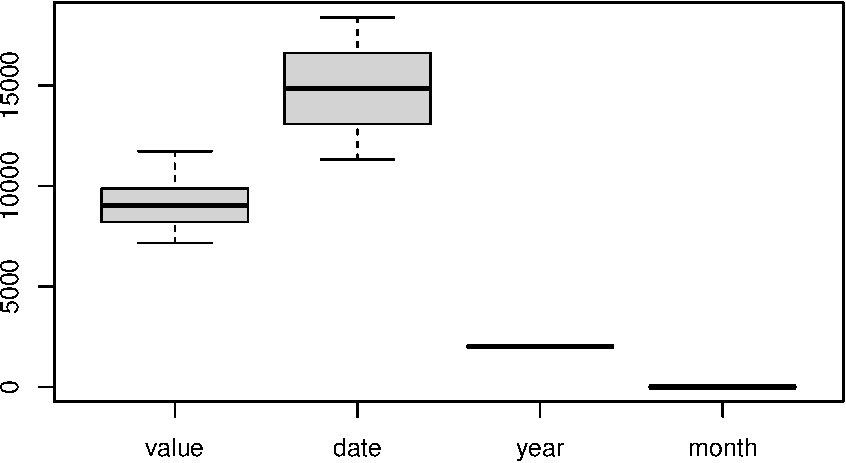
\includegraphics{graphics/make basic data summaries-1.pdf}

\begin{Shaded}
\begin{Highlighting}[]
\FunctionTok{hist}\NormalTok{(esales}\SpecialCharTok{$}\NormalTok{value, }\AttributeTok{breaks=}\DecValTok{40}\NormalTok{) }\CommentTok{\#  Make a histogram of monthly sales}
\end{Highlighting}
\end{Shaded}

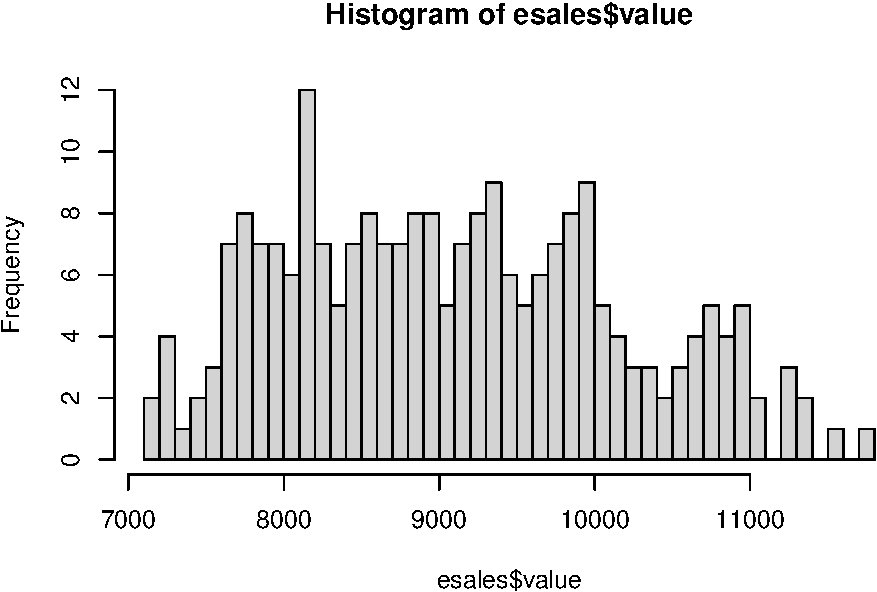
\includegraphics{graphics/make basic data summaries-2.pdf}

\hypertarget{examine-subsets-of-the-data}{%
\subsection{Examine subsets of the data}\label{examine-subsets-of-the-data}}

\begin{Shaded}
\begin{Highlighting}[]
\CommentTok{\# References: https://www.tidyverse.org/, https://dplyr.tidyverse.org/}
\CommentTok{\# filter(data object, condition) : syntax for filter() command}

\NormalTok{esales }\SpecialCharTok{\%\textgreater{}\%}
  \FunctionTok{filter}\NormalTok{(year }\SpecialCharTok{==} \DecValTok{2019}\NormalTok{) }\SpecialCharTok{\%\textgreater{}\%}
  \FunctionTok{filter}\NormalTok{(value }\SpecialCharTok{\textgreater{}} \DecValTok{9000}\NormalTok{) }\SpecialCharTok{\%\textgreater{}\%}
  \FunctionTok{print}\NormalTok{()}

\NormalTok{(esales }\SpecialCharTok{\%\textgreater{}\%}
  \FunctionTok{group\_by}\NormalTok{(year) }\SpecialCharTok{\%\textgreater{}\%}
  \FunctionTok{summarise}\NormalTok{(}\AttributeTok{Total =} \FunctionTok{sum}\NormalTok{(value)) }\OtherTok{{-}\textgreater{}}\NormalTok{ total\_esales\_by\_year)}

\NormalTok{esales }\SpecialCharTok{\%\textgreater{}\%}
  \FunctionTok{mutate}\NormalTok{(}\AttributeTok{sales\_TWh =}\NormalTok{ value}\SpecialCharTok{/}\DecValTok{1000}\NormalTok{) }\SpecialCharTok{\%\textgreater{}\%}
\NormalTok{  dplyr}\SpecialCharTok{::}\FunctionTok{select}\NormalTok{(}\SpecialCharTok{{-}}\NormalTok{value)}
\end{Highlighting}
\end{Shaded}

\begin{Shaded}
\begin{Highlighting}[]
\CommentTok{\# library(lubridate) \# Make it easy to deal with dates}

\NormalTok{esales }\SpecialCharTok{\%\textgreater{}\%} \FunctionTok{filter}\NormalTok{(month}\SpecialCharTok{==}\DecValTok{3}\NormalTok{)                   }\CommentTok{\# These three lines of code}
\end{Highlighting}
\end{Shaded}

\begin{verbatim}
## # A tibble: 20 x 4
##    value date        year month
##    <dbl> <date>     <int> <int>
##  1 8889. 2020-03-01  2020     3
##  2 9466. 2019-03-01  2019     3
##  3 9666. 2018-03-01  2018     3
##  4 9372. 2017-03-01  2017     3
##  5 8406. 2016-03-01  2016     3
##  6 9435. 2015-03-01  2015     3
##  7 9676. 2014-03-01  2014     3
##  8 9506. 2013-03-01  2013     3
##  9 8086. 2012-03-01  2012     3
## 10 8688. 2011-03-01  2011     3
## 11 8568. 2010-03-01  2010     3
## 12 8926. 2009-03-01  2009     3
## 13 8512. 2008-03-01  2008     3
## 14 8632. 2007-03-01  2007     3
## 15 8519. 2006-03-01  2006     3
## 16 9125. 2005-03-01  2005     3
## 17 8136. 2004-03-01  2004     3
## 18 8108. 2003-03-01  2003     3
## 19 7675. 2002-03-01  2002     3
## 20 8070. 2001-03-01  2001     3
\end{verbatim}

\begin{Shaded}
\begin{Highlighting}[]
\NormalTok{esales }\SpecialCharTok{\%\textgreater{}\%} \FunctionTok{filter}\NormalTok{(}\FunctionTok{month}\NormalTok{(date)}\SpecialCharTok{==}\DecValTok{3}\NormalTok{)             }\CommentTok{\#   all do}
\end{Highlighting}
\end{Shaded}

\begin{verbatim}
## # A tibble: 20 x 4
##    value date        year month
##    <dbl> <date>     <int> <int>
##  1 8889. 2020-03-01  2020     3
##  2 9466. 2019-03-01  2019     3
##  3 9666. 2018-03-01  2018     3
##  4 9372. 2017-03-01  2017     3
##  5 8406. 2016-03-01  2016     3
##  6 9435. 2015-03-01  2015     3
##  7 9676. 2014-03-01  2014     3
##  8 9506. 2013-03-01  2013     3
##  9 8086. 2012-03-01  2012     3
## 10 8688. 2011-03-01  2011     3
## 11 8568. 2010-03-01  2010     3
## 12 8926. 2009-03-01  2009     3
## 13 8512. 2008-03-01  2008     3
## 14 8632. 2007-03-01  2007     3
## 15 8519. 2006-03-01  2006     3
## 16 9125. 2005-03-01  2005     3
## 17 8136. 2004-03-01  2004     3
## 18 8108. 2003-03-01  2003     3
## 19 7675. 2002-03-01  2002     3
## 20 8070. 2001-03-01  2001     3
\end{verbatim}

\begin{Shaded}
\begin{Highlighting}[]
\NormalTok{esales }\SpecialCharTok{\%\textgreater{}\%} \FunctionTok{filter}\NormalTok{(lubridate}\SpecialCharTok{::}\FunctionTok{month}\NormalTok{(date)}\SpecialCharTok{==}\DecValTok{3}\NormalTok{)  }\CommentTok{\#   the same thing.}
\end{Highlighting}
\end{Shaded}

\begin{verbatim}
## # A tibble: 20 x 4
##    value date        year month
##    <dbl> <date>     <int> <int>
##  1 8889. 2020-03-01  2020     3
##  2 9466. 2019-03-01  2019     3
##  3 9666. 2018-03-01  2018     3
##  4 9372. 2017-03-01  2017     3
##  5 8406. 2016-03-01  2016     3
##  6 9435. 2015-03-01  2015     3
##  7 9676. 2014-03-01  2014     3
##  8 9506. 2013-03-01  2013     3
##  9 8086. 2012-03-01  2012     3
## 10 8688. 2011-03-01  2011     3
## 11 8568. 2010-03-01  2010     3
## 12 8926. 2009-03-01  2009     3
## 13 8512. 2008-03-01  2008     3
## 14 8632. 2007-03-01  2007     3
## 15 8519. 2006-03-01  2006     3
## 16 9125. 2005-03-01  2005     3
## 17 8136. 2004-03-01  2004     3
## 18 8108. 2003-03-01  2003     3
## 19 7675. 2002-03-01  2002     3
## 20 8070. 2001-03-01  2001     3
\end{verbatim}

\begin{Shaded}
\begin{Highlighting}[]
\CommentTok{\# We don\textquotesingle{}t have to keep the \textquotesingle{}year\textquotesingle{} and \textquotesingle{}month\textquotesingle{} column: can recover them if needed}

\NormalTok{esales }\SpecialCharTok{\%\textgreater{}\%}
\NormalTok{  dplyr}\SpecialCharTok{::}\FunctionTok{select}\NormalTok{(date, }\AttributeTok{sales\_GWh =}\NormalTok{ value) }\OtherTok{{-}\textgreater{}}\NormalTok{ esales\_tbl}

\FunctionTok{print}\NormalTok{(esales\_tbl)}
\end{Highlighting}
\end{Shaded}

\begin{verbatim}
## # A tibble: 233 x 2
##    date       sales_GWh
##    <date>         <dbl>
##  1 2020-05-01     8282.
##  2 2020-04-01     7839.
##  3 2020-03-01     8889.
##  4 2020-02-01     9368.
##  5 2020-01-01     9209.
##  6 2019-12-01    10038.
##  7 2019-11-01     9291.
##  8 2019-10-01     8757.
##  9 2019-09-01     9874.
## 10 2019-08-01    10912.
## # ... with 223 more rows
\end{verbatim}

\hypertarget{plot-the-time-series}{%
\section{Plot the time series}\label{plot-the-time-series}}

Ref: FPP3, Section 2.2

\begin{Shaded}
\begin{Highlighting}[]
\CommentTok{\#Reference: https://ggplot2.tidyverse.org/}

\FunctionTok{ggplot}\NormalTok{(}\AttributeTok{data=}\NormalTok{esales, }\FunctionTok{aes}\NormalTok{(}\AttributeTok{x=}\NormalTok{date,}\AttributeTok{y=}\NormalTok{value)) }\SpecialCharTok{+}
  \FunctionTok{geom\_line}\NormalTok{() }\SpecialCharTok{+} \FunctionTok{xlab}\NormalTok{(}\StringTok{"Year"}\NormalTok{) }\SpecialCharTok{+} \FunctionTok{ylab}\NormalTok{(}\StringTok{"Virginia monthly total electricity sales (GWh)"}\NormalTok{)}
\end{Highlighting}
\end{Shaded}

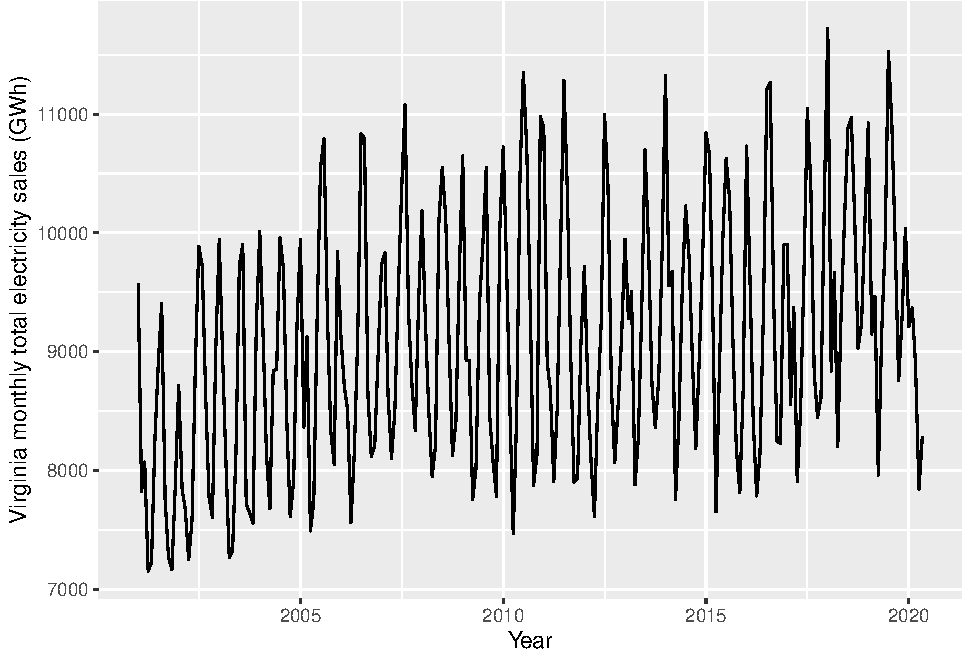
\includegraphics{graphics/use ggplot2 to generate a plot-1.pdf}

\hypertarget{sesaonal-plots}{%
\section{Sesaonal plots}\label{sesaonal-plots}}

Ref: FPP3, Sections 2.3, 2.4

\hypertarget{example-virginia-monthly-electricity}{%
\subsection{Example: Virginia monthly electricity}\label{example-virginia-monthly-electricity}}

Recall how we readied these data:

\begin{Shaded}
\begin{Highlighting}[]
\NormalTok{esales }\OtherTok{\textless{}{-}}\NormalTok{ arrow}\SpecialCharTok{::}\FunctionTok{read\_feather}\NormalTok{(}\StringTok{"data/esales.feather"}\NormalTok{)}
\NormalTok{esales }\SpecialCharTok{\%\textgreater{}\%}
\NormalTok{  dplyr}\SpecialCharTok{::}\FunctionTok{select}\NormalTok{(date, }\AttributeTok{sales\_GWh =}\NormalTok{ value) }\OtherTok{{-}\textgreater{}}\NormalTok{ esales\_tbl}

\NormalTok{esales\_tbl }\SpecialCharTok{\%\textgreater{}\%} \FunctionTok{as\_tsibble}\NormalTok{(}\AttributeTok{index =}\NormalTok{ date) }\OtherTok{{-}\textgreater{}}\NormalTok{ elsales\_tbl\_ts}

\FunctionTok{print}\NormalTok{(elsales\_tbl\_ts)}
\end{Highlighting}
\end{Shaded}

\begin{verbatim}
## # A tsibble: 233 x 2 [1D]
##    date       sales_GWh
##    <date>         <dbl>
##  1 2001-01-01     9576.
##  2 2001-02-01     7820.
##  3 2001-03-01     8070.
##  4 2001-04-01     7153.
##  5 2001-05-01     7224.
##  6 2001-06-01     8264.
##  7 2001-07-01     8896.
##  8 2001-08-01     9404.
##  9 2001-09-01     7753.
## 10 2001-10-01     7272.
## # ... with 223 more rows
\end{verbatim}

\begin{Shaded}
\begin{Highlighting}[]
\DocumentationTok{\#\#\# This plot won\textquotesingle{}t work. Why not?}
\CommentTok{\# elsales\_tbl\_ts \%\textgreater{}\%}
\CommentTok{\#   feasts::gg\_season(sales\_GWh, labels = "both") + ylab("Virginia electricity sales (GWh)")}
\end{Highlighting}
\end{Shaded}

\begin{Shaded}
\begin{Highlighting}[]
\CommentTok{\# install.packages("feasts"), Reference: https://feasts.tidyverts.org/}
\FunctionTok{library}\NormalTok{(feasts)}

\NormalTok{elsales\_tbl\_ts }\SpecialCharTok{\%\textgreater{}\%}
  \FunctionTok{mutate}\NormalTok{(}\AttributeTok{Month =}\NormalTok{ tsibble}\SpecialCharTok{::}\FunctionTok{yearmonth}\NormalTok{(date)) }\SpecialCharTok{\%\textgreater{}\%}
  \FunctionTok{as\_tsibble}\NormalTok{(}\AttributeTok{index =}\NormalTok{ Month) }\SpecialCharTok{\%\textgreater{}\%}
\NormalTok{  dplyr}\SpecialCharTok{::}\FunctionTok{select}\NormalTok{(Month,sales\_GWh) }\OtherTok{{-}\textgreater{}}\NormalTok{ vaelsales\_tbl\_ts}

\FunctionTok{print}\NormalTok{(vaelsales\_tbl\_ts)}
\end{Highlighting}
\end{Shaded}

\begin{verbatim}
## # A tsibble: 233 x 2 [1M]
##       Month sales_GWh
##       <mth>     <dbl>
##  1 2001 Jan     9576.
##  2 2001 Feb     7820.
##  3 2001 Mar     8070.
##  4 2001 Apr     7153.
##  5 2001 May     7224.
##  6 2001 Jun     8264.
##  7 2001 Jul     8896.
##  8 2001 Aug     9404.
##  9 2001 Sep     7753.
## 10 2001 Oct     7272.
## # ... with 223 more rows
\end{verbatim}

\begin{Shaded}
\begin{Highlighting}[]
\CommentTok{\# feasts::autoplot() is handy for quickly generating time series plots}

\FunctionTok{autoplot}\NormalTok{(vaelsales\_tbl\_ts, sales\_GWh) }\SpecialCharTok{+}
  \FunctionTok{ylab}\NormalTok{(}\StringTok{"Virginia monthly total electricity sales (GWh)"}\NormalTok{) }\SpecialCharTok{+}
  \FunctionTok{xlab}\NormalTok{(}\StringTok{""}\NormalTok{)  }\CommentTok{\# Leave horiz. axis label blank}
\end{Highlighting}
\end{Shaded}

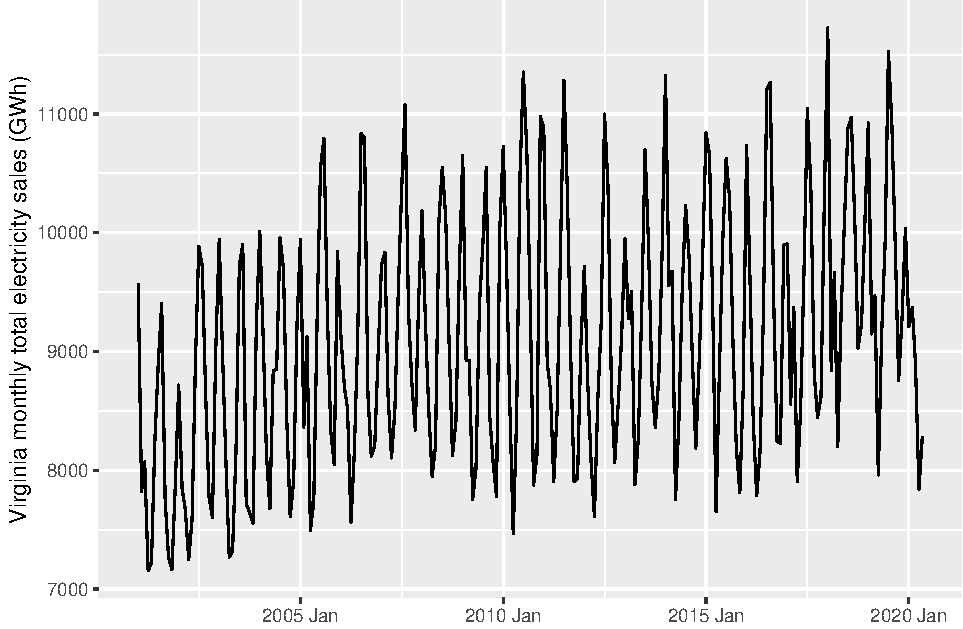
\includegraphics{graphics/use feasts autoplot-1.pdf}

\begin{Shaded}
\begin{Highlighting}[]
\NormalTok{vaelsales\_tbl\_ts }\SpecialCharTok{\%\textgreater{}\%} \FunctionTok{gg\_season}\NormalTok{(sales\_GWh, }\AttributeTok{labels =} \StringTok{"both"}\NormalTok{) }\SpecialCharTok{+} \FunctionTok{ylab}\NormalTok{(}\StringTok{"Virginia electricity sales (GWh)"}\NormalTok{)}
\end{Highlighting}
\end{Shaded}

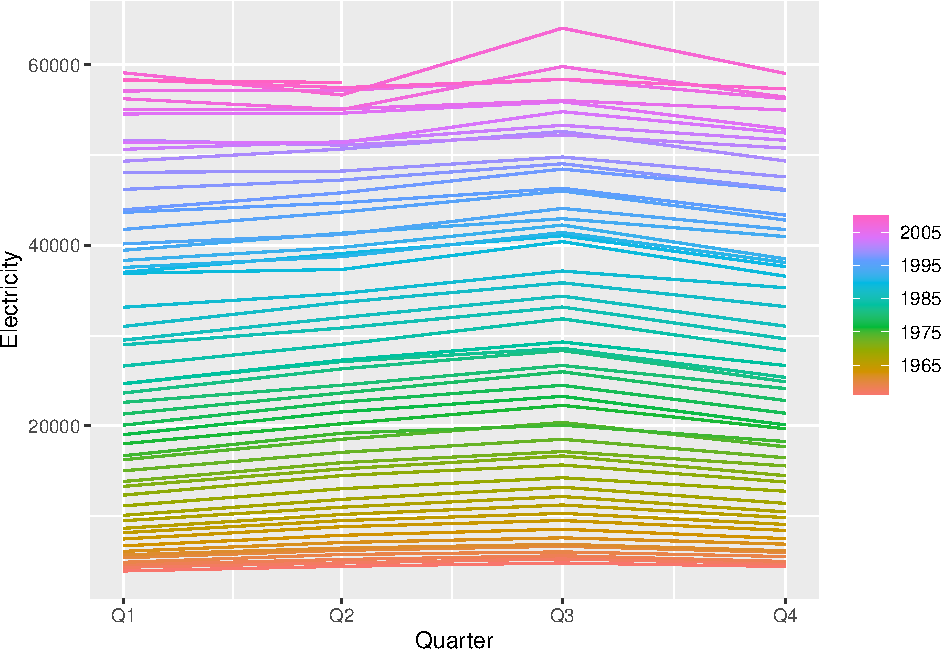
\includegraphics{graphics/unnamed-chunk-16-1.pdf}

\hypertarget{example-australian-production}{%
\subsection{Example: Australian production}\label{example-australian-production}}

\begin{Shaded}
\begin{Highlighting}[]
\CommentTok{\# install.packages(\textquotesingle{}tsibbledata\textquotesingle{})}
\FunctionTok{library}\NormalTok{(tsibbledata)}

\NormalTok{aus\_production}
\end{Highlighting}
\end{Shaded}

\begin{verbatim}
## # A tsibble: 218 x 7 [1Q]
##    Quarter  Beer Tobacco Bricks Cement Electricity   Gas
##      <qtr> <dbl>   <dbl>  <dbl>  <dbl>       <dbl> <dbl>
##  1 1956 Q1   284    5225    189    465        3923     5
##  2 1956 Q2   213    5178    204    532        4436     6
##  3 1956 Q3   227    5297    208    561        4806     7
##  4 1956 Q4   308    5681    197    570        4418     6
##  5 1957 Q1   262    5577    187    529        4339     5
##  6 1957 Q2   228    5651    214    604        4811     7
##  7 1957 Q3   236    5317    227    603        5259     7
##  8 1957 Q4   320    6152    222    582        4735     6
##  9 1958 Q1   272    5758    199    554        4608     5
## 10 1958 Q2   233    5641    229    620        5196     7
## # ... with 208 more rows
\end{verbatim}

\begin{Shaded}
\begin{Highlighting}[]
\NormalTok{aus\_production }\SpecialCharTok{\%\textgreater{}\%} \FunctionTok{gg\_season}\NormalTok{(Electricity)}
\end{Highlighting}
\end{Shaded}

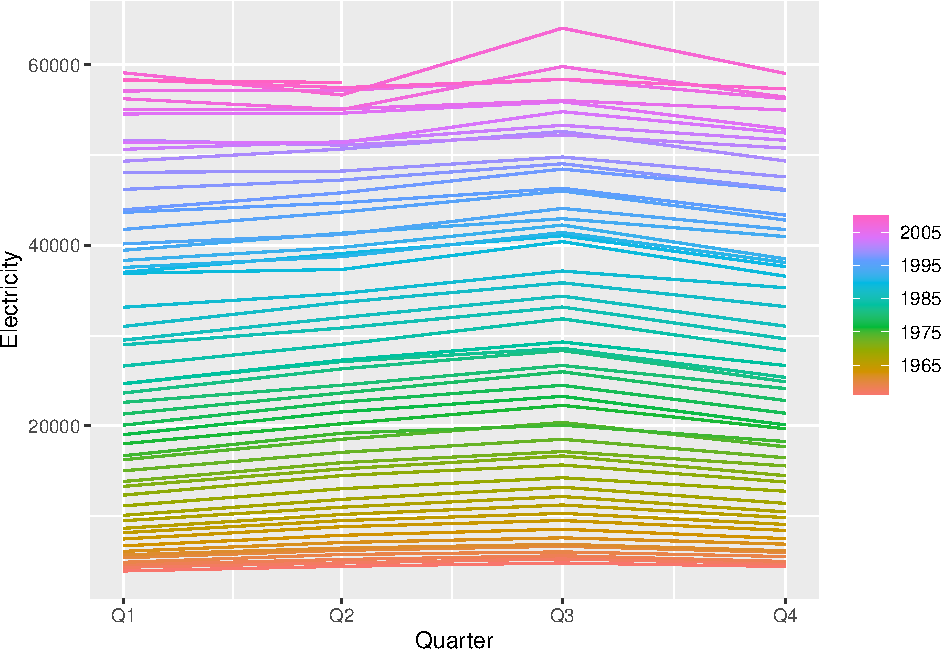
\includegraphics{graphics/unnamed-chunk-17-1.pdf}

\begin{Shaded}
\begin{Highlighting}[]
\NormalTok{aus\_production }\SpecialCharTok{\%\textgreater{}\%} \FunctionTok{gg\_season}\NormalTok{(Beer)}
\end{Highlighting}
\end{Shaded}

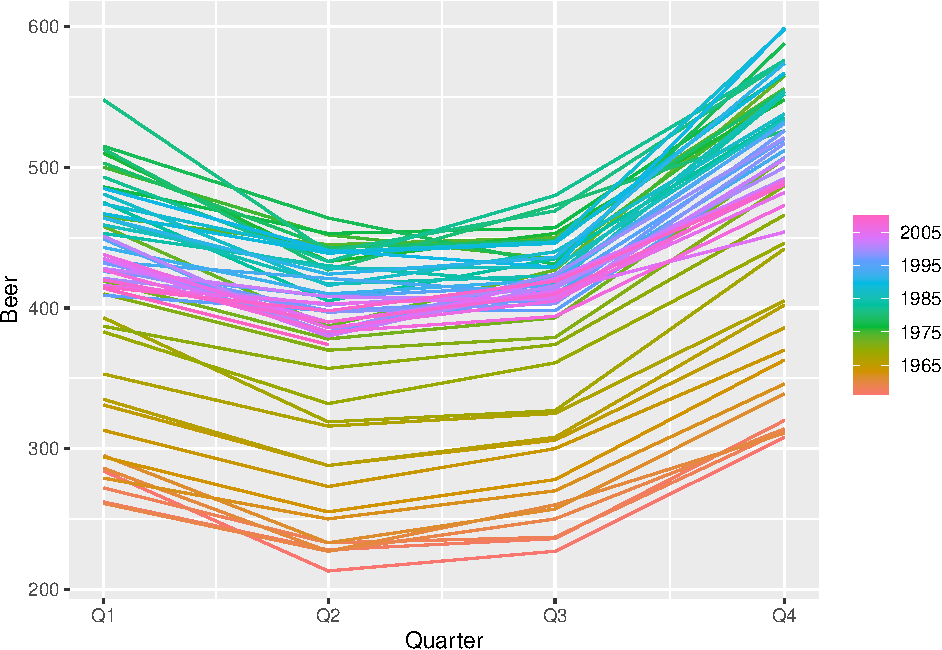
\includegraphics{graphics/unnamed-chunk-17-2.pdf}

\hypertarget{seasonal-subseries-plots}{%
\subsection{Seasonal subseries plots}\label{seasonal-subseries-plots}}

Ref: FPP3, Section 2.5

\begin{Shaded}
\begin{Highlighting}[]
\NormalTok{vaelsales\_tbl\_ts }\SpecialCharTok{\%\textgreater{}\%}
  \FunctionTok{gg\_subseries}\NormalTok{(sales\_GWh) }\SpecialCharTok{+}
  \FunctionTok{labs}\NormalTok{(}
    \AttributeTok{y =} \StringTok{"Sales (GWh)"}\NormalTok{,}
    \AttributeTok{title =} \StringTok{"Seasonal subseries plot: Virginia electricity sales"}
\NormalTok{  )}
\end{Highlighting}
\end{Shaded}

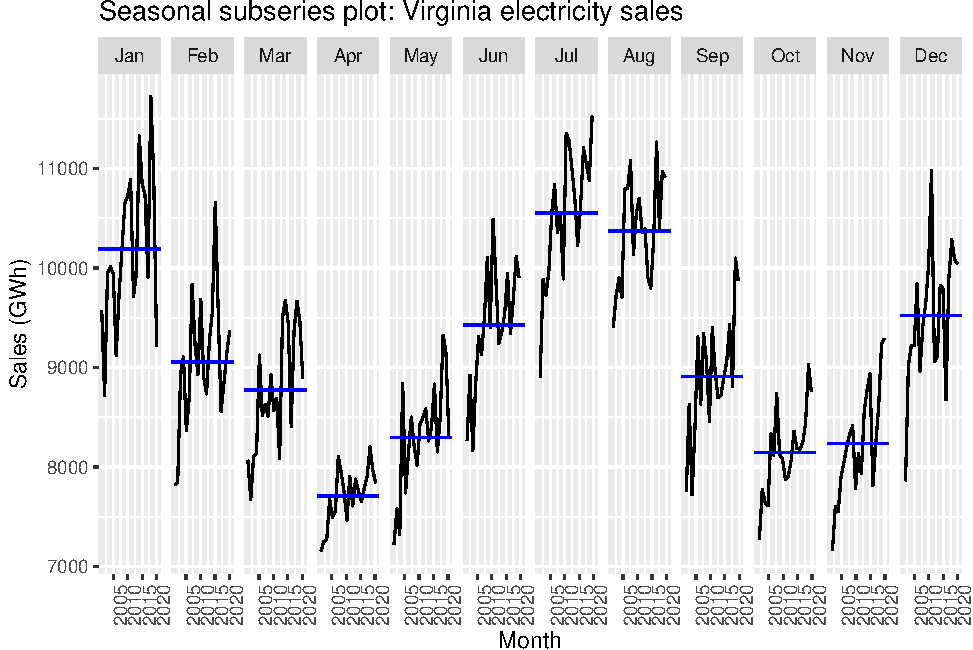
\includegraphics{graphics/unnamed-chunk-18-1.pdf}

\hypertarget{scatterplots}{%
\section{Scatterplots}\label{scatterplots}}

Readings: FPP Sect. 2.6

Investigating relationships between two variables. Scatterplots. Correlation. Scatterplot matrices.

\begin{Shaded}
\begin{Highlighting}[]
\NormalTok{vic\_elec}
\end{Highlighting}
\end{Shaded}

\begin{verbatim}
## # A tsibble: 52,608 x 5 [30m] <Australia/Melbourne>
##    Time                Demand Temperature Date       Holiday
##    <dttm>               <dbl>       <dbl> <date>     <lgl>  
##  1 2012-01-01 00:00:00  4383.        21.4 2012-01-01 TRUE   
##  2 2012-01-01 00:30:00  4263.        21.0 2012-01-01 TRUE   
##  3 2012-01-01 01:00:00  4049.        20.7 2012-01-01 TRUE   
##  4 2012-01-01 01:30:00  3878.        20.6 2012-01-01 TRUE   
##  5 2012-01-01 02:00:00  4036.        20.4 2012-01-01 TRUE   
##  6 2012-01-01 02:30:00  3866.        20.2 2012-01-01 TRUE   
##  7 2012-01-01 03:00:00  3694.        20.1 2012-01-01 TRUE   
##  8 2012-01-01 03:30:00  3562.        19.6 2012-01-01 TRUE   
##  9 2012-01-01 04:00:00  3433.        19.1 2012-01-01 TRUE   
## 10 2012-01-01 04:30:00  3359.        19.0 2012-01-01 TRUE   
## # ... with 52,598 more rows
\end{verbatim}

\begin{Shaded}
\begin{Highlighting}[]
\FunctionTok{summary}\NormalTok{(vic\_elec)}
\end{Highlighting}
\end{Shaded}

\begin{verbatim}
##       Time                         Demand      Temperature   
##  Min.   :2012-01-01 00:00:00   Min.   :2858   Min.   : 1.50  
##  1st Qu.:2012-09-30 22:52:30   1st Qu.:3969   1st Qu.:12.30  
##  Median :2013-07-01 22:45:00   Median :4635   Median :15.40  
##  Mean   :2013-07-01 22:45:00   Mean   :4665   Mean   :16.27  
##  3rd Qu.:2014-04-01 23:37:30   3rd Qu.:5244   3rd Qu.:19.40  
##  Max.   :2014-12-31 23:30:00   Max.   :9345   Max.   :43.20  
##       Date             Holiday       
##  Min.   :2012-01-01   Mode :logical  
##  1st Qu.:2012-09-30   FALSE:51120    
##  Median :2013-07-01   TRUE :1488     
##  Mean   :2013-07-01                  
##  3rd Qu.:2014-04-01                  
##  Max.   :2014-12-31
\end{verbatim}

\begin{Shaded}
\begin{Highlighting}[]
\NormalTok{vic\_elec }\SpecialCharTok{\%\textgreater{}\%}
  \FunctionTok{filter}\NormalTok{(}\FunctionTok{year}\NormalTok{(Time) }\SpecialCharTok{==} \DecValTok{2013}\NormalTok{) }\SpecialCharTok{\%\textgreater{}\%}
  \FunctionTok{autoplot}\NormalTok{(Demand) }\SpecialCharTok{+}
  \FunctionTok{labs}\NormalTok{(}
    \AttributeTok{y =} \StringTok{"Demand (GW)"}\NormalTok{,}
    \AttributeTok{title =} \StringTok{"Half{-}hourly electricity demand: Victoria"}
\NormalTok{  )}
\end{Highlighting}
\end{Shaded}

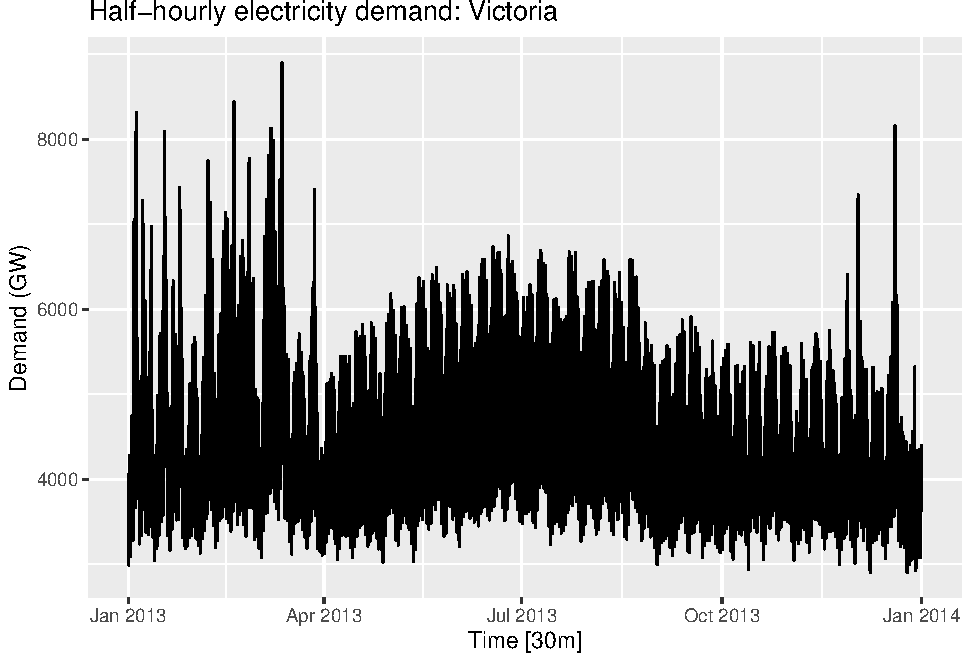
\includegraphics{graphics/unnamed-chunk-19-1.pdf}

\begin{Shaded}
\begin{Highlighting}[]
\NormalTok{vic\_elec }\SpecialCharTok{\%\textgreater{}\%}
  \FunctionTok{filter}\NormalTok{(}\FunctionTok{year}\NormalTok{(Time) }\SpecialCharTok{==} \DecValTok{2013}\NormalTok{) }\SpecialCharTok{\%\textgreater{}\%}
  \FunctionTok{autoplot}\NormalTok{(Temperature) }\SpecialCharTok{+}
  \FunctionTok{labs}\NormalTok{(}
    \AttributeTok{y =} \StringTok{"Temperature (degrees Celsius)"}\NormalTok{,}
    \AttributeTok{title =} \StringTok{"Half{-}hourly temperatures: Melbourne, Australia"}
\NormalTok{  )}
\end{Highlighting}
\end{Shaded}

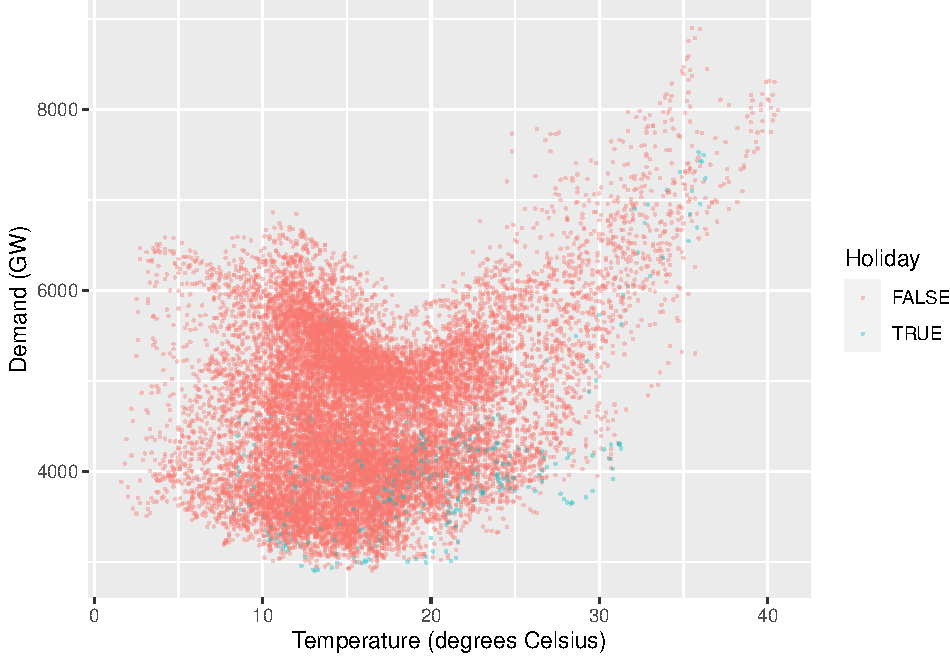
\includegraphics{graphics/unnamed-chunk-20-1.pdf}

\begin{Shaded}
\begin{Highlighting}[]
\NormalTok{vic\_elec }\SpecialCharTok{\%\textgreater{}\%}
  \FunctionTok{filter}\NormalTok{(}\FunctionTok{year}\NormalTok{(Time) }\SpecialCharTok{==} \DecValTok{2013}\NormalTok{) }\SpecialCharTok{\%\textgreater{}\%}
  \FunctionTok{ggplot}\NormalTok{(}\FunctionTok{aes}\NormalTok{(}\AttributeTok{x =}\NormalTok{ Temperature, }\AttributeTok{y =}\NormalTok{ Demand)) }\SpecialCharTok{+}
\CommentTok{\#  geom\_density2d() +}
  \FunctionTok{geom\_point}\NormalTok{(}\AttributeTok{size=}\FloatTok{0.1}\NormalTok{, }\FunctionTok{aes}\NormalTok{(}\AttributeTok{colour=}\NormalTok{Holiday), }\AttributeTok{alpha =} \FloatTok{0.4}\NormalTok{) }\SpecialCharTok{+}
  \FunctionTok{labs}\NormalTok{(}\AttributeTok{y =} \StringTok{"Demand (GW)"}\NormalTok{, }\AttributeTok{x =} \StringTok{"Temperature (degrees Celsius)"}\NormalTok{)}
\end{Highlighting}
\end{Shaded}

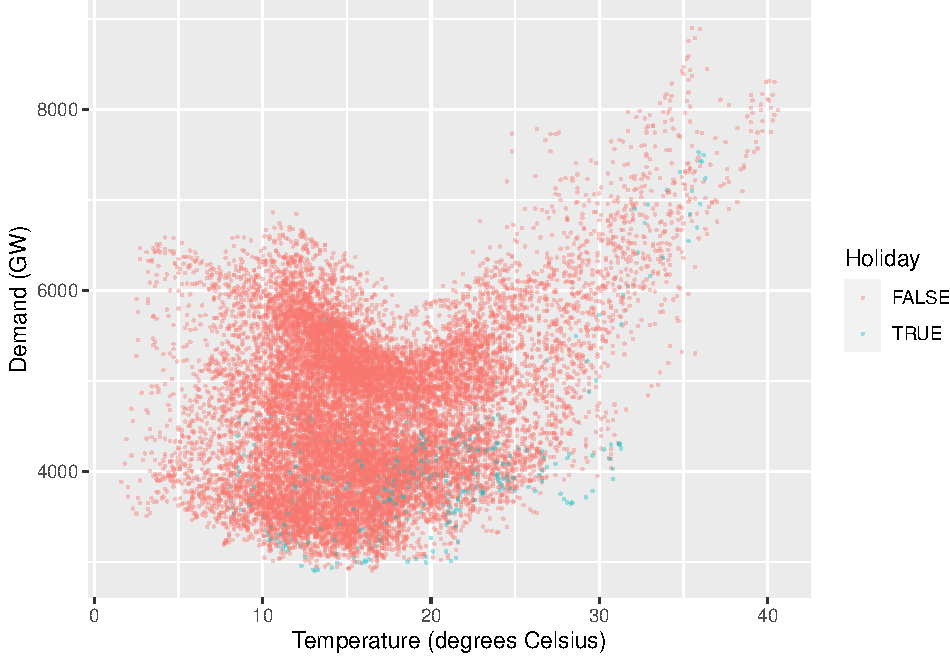
\includegraphics{graphics/unnamed-chunk-21-1.pdf}

\hypertarget{a-scatterplot-matrix}{%
\subsection{A Scatterplot matrix}\label{a-scatterplot-matrix}}

\begin{Shaded}
\begin{Highlighting}[]
\NormalTok{vic\_elec}
\end{Highlighting}
\end{Shaded}

\begin{verbatim}
## # A tsibble: 52,608 x 5 [30m] <Australia/Melbourne>
##    Time                Demand Temperature Date       Holiday
##    <dttm>               <dbl>       <dbl> <date>     <lgl>  
##  1 2012-01-01 00:00:00  4383.        21.4 2012-01-01 TRUE   
##  2 2012-01-01 00:30:00  4263.        21.0 2012-01-01 TRUE   
##  3 2012-01-01 01:00:00  4049.        20.7 2012-01-01 TRUE   
##  4 2012-01-01 01:30:00  3878.        20.6 2012-01-01 TRUE   
##  5 2012-01-01 02:00:00  4036.        20.4 2012-01-01 TRUE   
##  6 2012-01-01 02:30:00  3866.        20.2 2012-01-01 TRUE   
##  7 2012-01-01 03:00:00  3694.        20.1 2012-01-01 TRUE   
##  8 2012-01-01 03:30:00  3562.        19.6 2012-01-01 TRUE   
##  9 2012-01-01 04:00:00  3433.        19.1 2012-01-01 TRUE   
## 10 2012-01-01 04:30:00  3359.        19.0 2012-01-01 TRUE   
## # ... with 52,598 more rows
\end{verbatim}

\begin{Shaded}
\begin{Highlighting}[]
\FunctionTok{boxplot}\NormalTok{(vic\_elec}\SpecialCharTok{$}\NormalTok{Temperature)}
\end{Highlighting}
\end{Shaded}

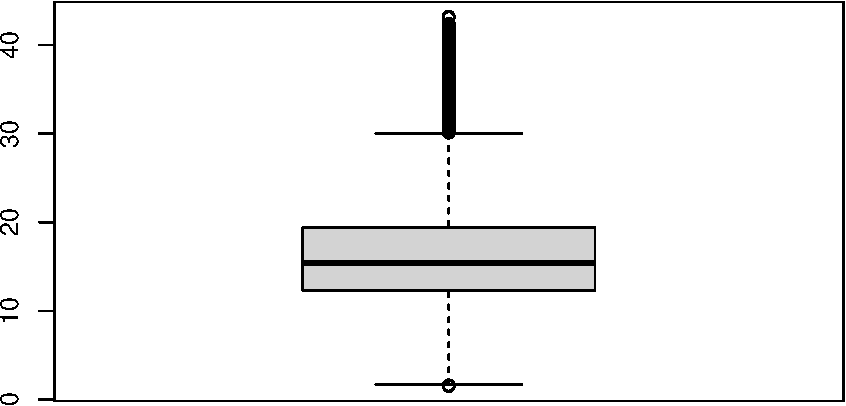
\includegraphics{graphics/unnamed-chunk-22-1.pdf}

\begin{Shaded}
\begin{Highlighting}[]
\CommentTok{\# install.packages("GGally")}
\NormalTok{vic\_elec }\SpecialCharTok{\%\textgreater{}\%}
  \CommentTok{\# mutate(Temperature = round(Temperature)) \%\textgreater{}\%}
  \CommentTok{\# pivot\_wider(values\_from=c(Demand,Temperature), names\_from=Holiday) \%\textgreater{}\%}
\NormalTok{  GGally}\SpecialCharTok{::}\FunctionTok{ggpairs}\NormalTok{(}\AttributeTok{columns =} \DecValTok{3}\SpecialCharTok{:}\DecValTok{2}\NormalTok{)}
\end{Highlighting}
\end{Shaded}

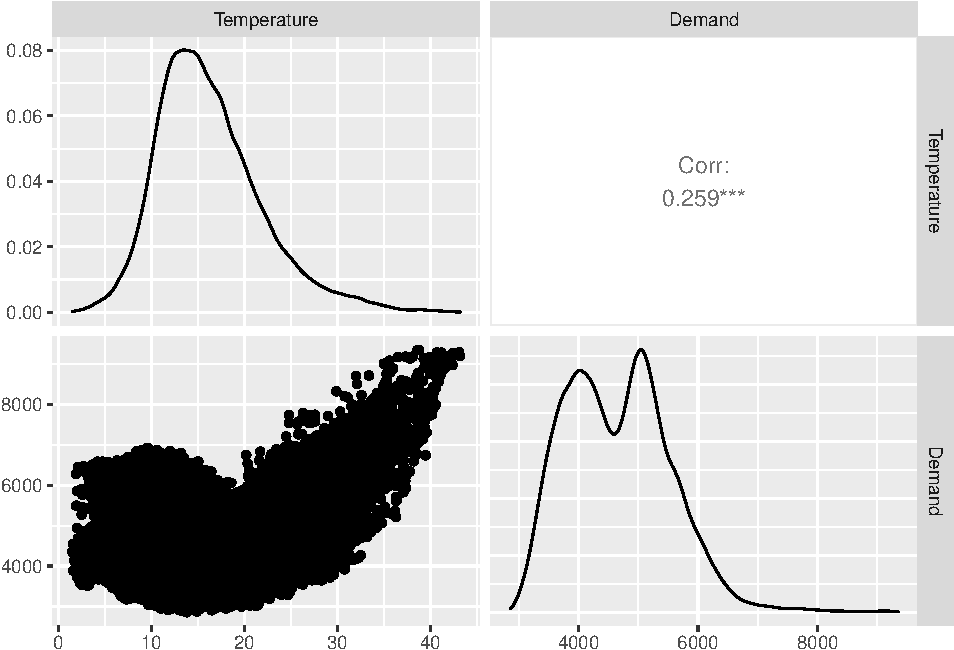
\includegraphics{graphics/unnamed-chunk-22-2.pdf}

\begin{Shaded}
\begin{Highlighting}[]
\NormalTok{vic\_elec }\SpecialCharTok{\%\textgreater{}\%}
  \FunctionTok{mutate}\NormalTok{(}\AttributeTok{Year =} \FunctionTok{factor}\NormalTok{(}\FunctionTok{year}\NormalTok{(Date))) }\SpecialCharTok{\%\textgreater{}\%}
\NormalTok{  dplyr}\SpecialCharTok{::}\FunctionTok{select}\NormalTok{(}\SpecialCharTok{{-}}\FunctionTok{c}\NormalTok{(Date, Holiday)) }\SpecialCharTok{\%\textgreater{}\%}
\NormalTok{  GGally}\SpecialCharTok{::}\FunctionTok{ggpairs}\NormalTok{(}\AttributeTok{columns =} \DecValTok{4}\SpecialCharTok{:}\DecValTok{2}\NormalTok{)}
\end{Highlighting}
\end{Shaded}

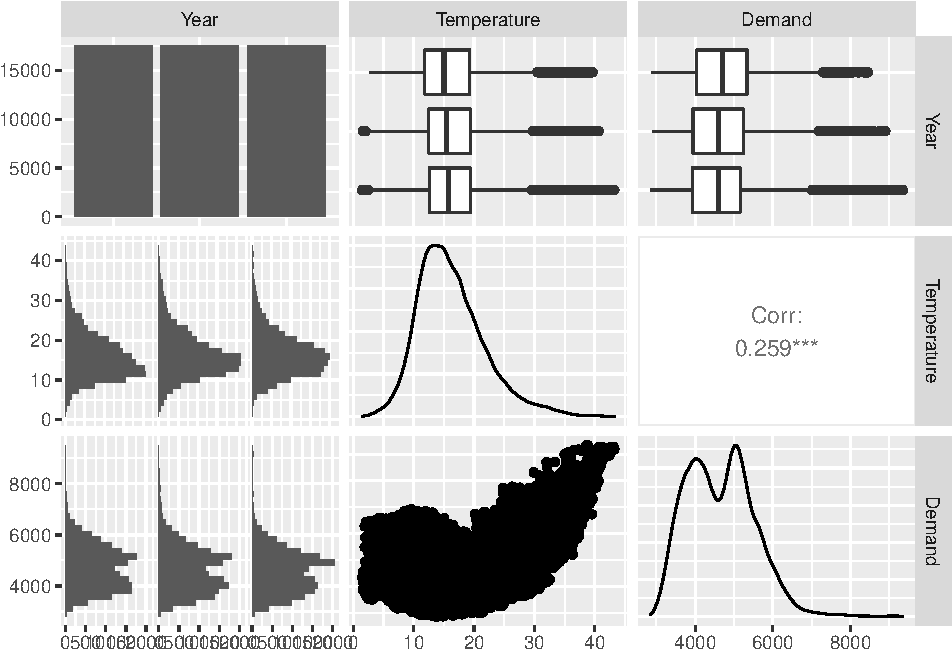
\includegraphics{graphics/unnamed-chunk-22-3.pdf}

\hypertarget{time-series-decomposition}{%
\chapter{Time series decomposition}\label{time-series-decomposition}}

Readings: FPP3, Sections 3.1, 3.2

\hypertarget{example-gross-domestic-product-data}{%
\subsection{Example: Gross Domestic Product data}\label{example-gross-domestic-product-data}}

\begin{Shaded}
\begin{Highlighting}[]
\FunctionTok{library}\NormalTok{(tsibbledata) }\CommentTok{\# Data sets package}

\FunctionTok{print}\NormalTok{(global\_economy)}
\end{Highlighting}
\end{Shaded}

\begin{verbatim}
## # A tsibble: 15,150 x 9 [1Y]
## # Key:       Country [263]
##    Country     Code   Year         GDP Growth   CPI Imports Exports Population
##    <fct>       <fct> <dbl>       <dbl>  <dbl> <dbl>   <dbl>   <dbl>      <dbl>
##  1 Afghanistan AFG    1960  537777811.     NA    NA    7.02    4.13    8996351
##  2 Afghanistan AFG    1961  548888896.     NA    NA    8.10    4.45    9166764
##  3 Afghanistan AFG    1962  546666678.     NA    NA    9.35    4.88    9345868
##  4 Afghanistan AFG    1963  751111191.     NA    NA   16.9     9.17    9533954
##  5 Afghanistan AFG    1964  800000044.     NA    NA   18.1     8.89    9731361
##  6 Afghanistan AFG    1965 1006666638.     NA    NA   21.4    11.3     9938414
##  7 Afghanistan AFG    1966 1399999967.     NA    NA   18.6     8.57   10152331
##  8 Afghanistan AFG    1967 1673333418.     NA    NA   14.2     6.77   10372630
##  9 Afghanistan AFG    1968 1373333367.     NA    NA   15.2     8.90   10604346
## 10 Afghanistan AFG    1969 1408888922.     NA    NA   15.0    10.1    10854428
## # ... with 15,140 more rows
\end{verbatim}

\begin{Shaded}
\begin{Highlighting}[]
\NormalTok{global\_economy }\SpecialCharTok{\%\textgreater{}\%} \FunctionTok{filter}\NormalTok{(Country}\SpecialCharTok{==}\StringTok{"Sweden"}\NormalTok{) }\SpecialCharTok{\%\textgreater{}\%} \FunctionTok{print}\NormalTok{()}
\end{Highlighting}
\end{Shaded}

\begin{verbatim}
## # A tsibble: 58 x 9 [1Y]
## # Key:       Country [1]
##    Country Code   Year          GDP Growth   CPI Imports Exports Population
##    <fct>   <fct> <dbl>        <dbl>  <dbl> <dbl>   <dbl>   <dbl>      <dbl>
##  1 Sweden  SWE    1960 14842870293.  NA     9.21    23.4    23.0    7484656
##  2 Sweden  SWE    1961 16147160123.   5.68  9.41    21.7    22.3    7519998
##  3 Sweden  SWE    1962 17511477311.   4.26  9.86    21.4    21.9    7561588
##  4 Sweden  SWE    1963 18954132366.   5.33 10.1     21.5    21.9    7604328
##  5 Sweden  SWE    1964 21137242561.   6.82 10.5     21.9    22.3    7661354
##  6 Sweden  SWE    1965 23260320646.   3.82 11.0     22.5    21.9    7733853
##  7 Sweden  SWE    1966 25302033132.   2.09 11.7     21.9    21.4    7807797
##  8 Sweden  SWE    1967 27463409202.   3.37 12.2     21.0    21.1    7867931
##  9 Sweden  SWE    1968 29143383491.   3.64 12.5     21.6    21.6    7912273
## 10 Sweden  SWE    1969 31649203886.   5.01 12.8     23.0    22.8    7968072
## # ... with 48 more rows
\end{verbatim}

\begin{Shaded}
\begin{Highlighting}[]
\NormalTok{global\_economy }\SpecialCharTok{\%\textgreater{}\%}
  \FunctionTok{filter}\NormalTok{(Country}\SpecialCharTok{==}\StringTok{"Sweden"}\NormalTok{) }\SpecialCharTok{\%\textgreater{}\%}
  \FunctionTok{autoplot}\NormalTok{(GDP) }\SpecialCharTok{+}
  \FunctionTok{ggtitle}\NormalTok{(}\StringTok{"GDP for Sweden"}\NormalTok{) }\SpecialCharTok{+} \FunctionTok{ylab}\NormalTok{(}\StringTok{"$US billions"}\NormalTok{)}
\end{Highlighting}
\end{Shaded}

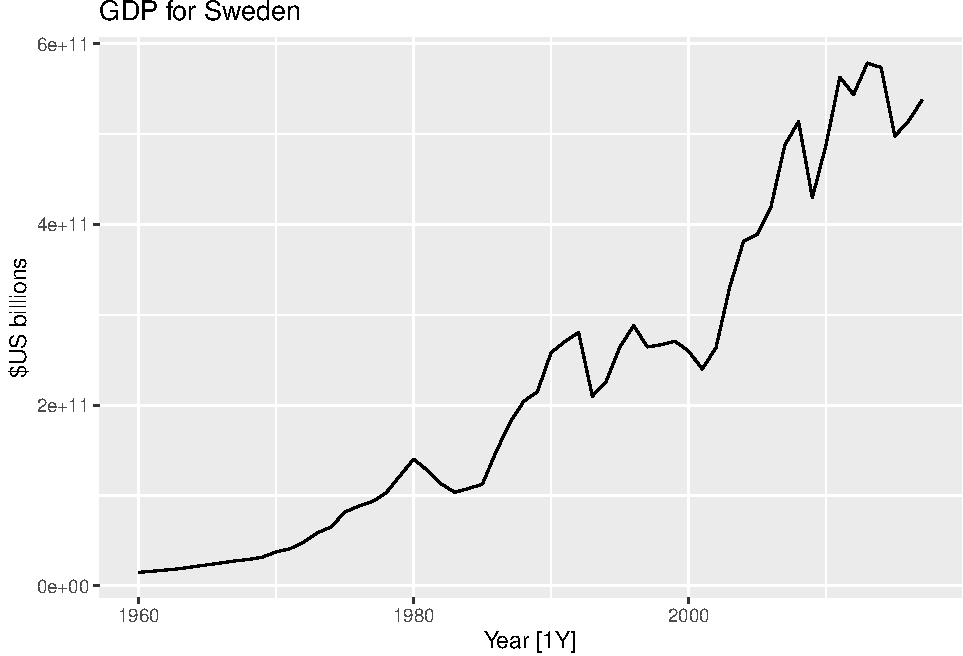
\includegraphics{graphics/unnamed-chunk-25-1.pdf}

\hypertarget{fitting-data-to-simple-models}{%
\subsection{Fitting data to simple models}\label{fitting-data-to-simple-models}}

\begin{Shaded}
\begin{Highlighting}[]
\NormalTok{global\_economy }\SpecialCharTok{\%\textgreater{}\%} \FunctionTok{model}\NormalTok{(}\AttributeTok{trend\_model =} \FunctionTok{TSLM}\NormalTok{(GDP }\SpecialCharTok{\textasciitilde{}} \FunctionTok{trend}\NormalTok{())) }\OtherTok{{-}\textgreater{}}\NormalTok{ fit}

\NormalTok{fit}
\end{Highlighting}
\end{Shaded}

\begin{verbatim}
## # A mable: 263 x 2
## # Key:     Country [263]
##    Country             trend_model
##    <fct>                   <model>
##  1 Afghanistan              <TSLM>
##  2 Albania                  <TSLM>
##  3 Algeria                  <TSLM>
##  4 American Samoa           <TSLM>
##  5 Andorra                  <TSLM>
##  6 Angola                   <TSLM>
##  7 Antigua and Barbuda      <TSLM>
##  8 Arab World               <TSLM>
##  9 Argentina                <TSLM>
## 10 Armenia                  <TSLM>
## # ... with 253 more rows
\end{verbatim}

\begin{Shaded}
\begin{Highlighting}[]
\NormalTok{fit }\SpecialCharTok{\%\textgreater{}\%} \FunctionTok{filter}\NormalTok{(Country }\SpecialCharTok{==} \StringTok{"Sweden"}\NormalTok{) }\SpecialCharTok{\%\textgreater{}\%} \FunctionTok{residuals}\NormalTok{()}
\end{Highlighting}
\end{Shaded}

\begin{verbatim}
## # A tsibble: 58 x 4 [1Y]
## # Key:       Country, .model [1]
##    Country .model       Year       .resid
##    <fct>   <chr>       <dbl>        <dbl>
##  1 Sweden  trend_model  1960 79973991821.
##  2 Sweden  trend_model  1961 71110300270.
##  3 Sweden  trend_model  1962 62306636078.
##  4 Sweden  trend_model  1963 53581309752.
##  5 Sweden  trend_model  1964 45596438566.
##  6 Sweden  trend_model  1965 37551535271.
##  7 Sweden  trend_model  1966 29425266377.
##  8 Sweden  trend_model  1967 21418661066.
##  9 Sweden  trend_model  1968 12930653974.
## 10 Sweden  trend_model  1969  5268492989.
## # ... with 48 more rows
\end{verbatim}

\begin{Shaded}
\begin{Highlighting}[]
\NormalTok{fit }\SpecialCharTok{\%\textgreater{}\%} \FunctionTok{filter}\NormalTok{(Country }\SpecialCharTok{==} \StringTok{"Sweden"}\NormalTok{) }\SpecialCharTok{\%\textgreater{}\%} \FunctionTok{residuals}\NormalTok{() }\SpecialCharTok{\%\textgreater{}\%} \FunctionTok{autoplot}\NormalTok{(.resid)}
\end{Highlighting}
\end{Shaded}

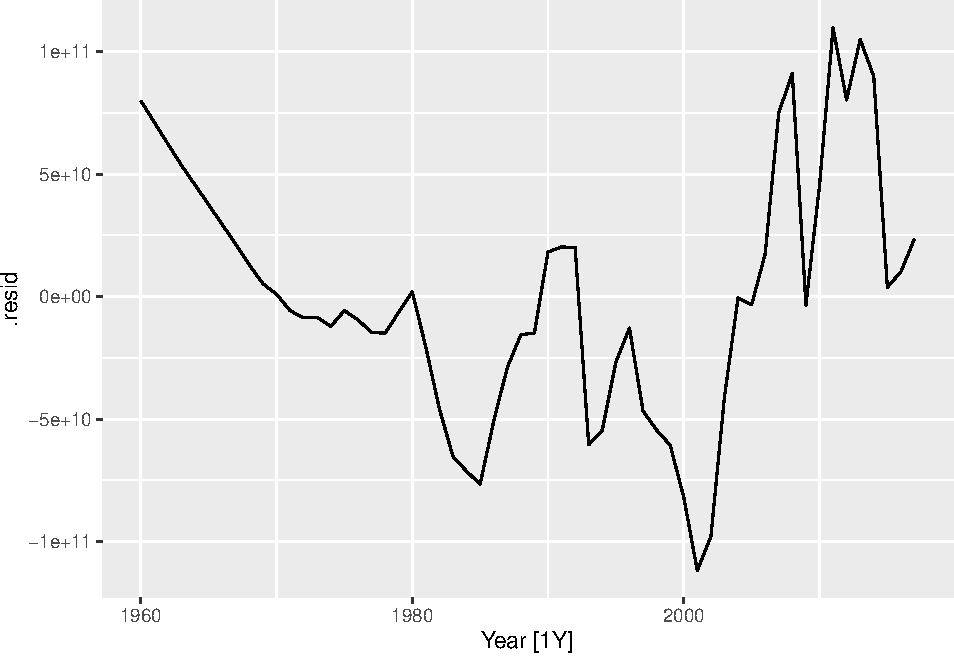
\includegraphics{graphics/unnamed-chunk-28-1.pdf}

\hypertarget{work-with-lngdp}{%
\subsection{Work with ln(GDP)}\label{work-with-lngdp}}

\begin{Shaded}
\begin{Highlighting}[]
\NormalTok{global\_economy }\SpecialCharTok{\%\textgreater{}\%}
  \FunctionTok{filter}\NormalTok{(Country}\SpecialCharTok{==}\StringTok{"Sweden"}\NormalTok{) }\SpecialCharTok{\%\textgreater{}\%}
  \FunctionTok{autoplot}\NormalTok{(}\FunctionTok{log}\NormalTok{(GDP)) }\SpecialCharTok{+}
  \FunctionTok{ggtitle}\NormalTok{(}\StringTok{"ln(GDP) for Sweden"}\NormalTok{) }\SpecialCharTok{+} \FunctionTok{ylab}\NormalTok{(}\StringTok{"$US billions"}\NormalTok{)}
\end{Highlighting}
\end{Shaded}

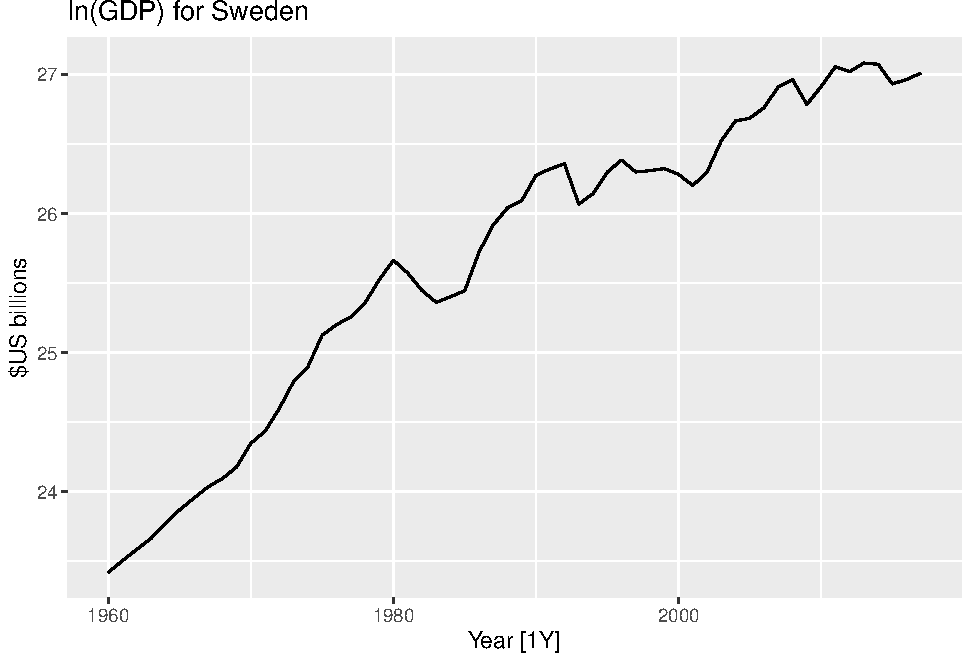
\includegraphics{graphics/unnamed-chunk-29-1.pdf}

\begin{Shaded}
\begin{Highlighting}[]
\NormalTok{global\_economy }\SpecialCharTok{\%\textgreater{}\%}
  \FunctionTok{model}\NormalTok{(}\AttributeTok{trend\_model =} \FunctionTok{TSLM}\NormalTok{(}\FunctionTok{log}\NormalTok{(GDP) }\SpecialCharTok{\textasciitilde{}} \FunctionTok{trend}\NormalTok{())) }\OtherTok{{-}\textgreater{}}\NormalTok{ logfit}
\end{Highlighting}
\end{Shaded}

\begin{Shaded}
\begin{Highlighting}[]
\NormalTok{logfit }\SpecialCharTok{\%\textgreater{}\%} \FunctionTok{filter}\NormalTok{(Country }\SpecialCharTok{==} \StringTok{"Sweden"}\NormalTok{) }\SpecialCharTok{\%\textgreater{}\%} \FunctionTok{residuals}\NormalTok{() }\SpecialCharTok{\%\textgreater{}\%} \FunctionTok{autoplot}\NormalTok{()}
\end{Highlighting}
\end{Shaded}

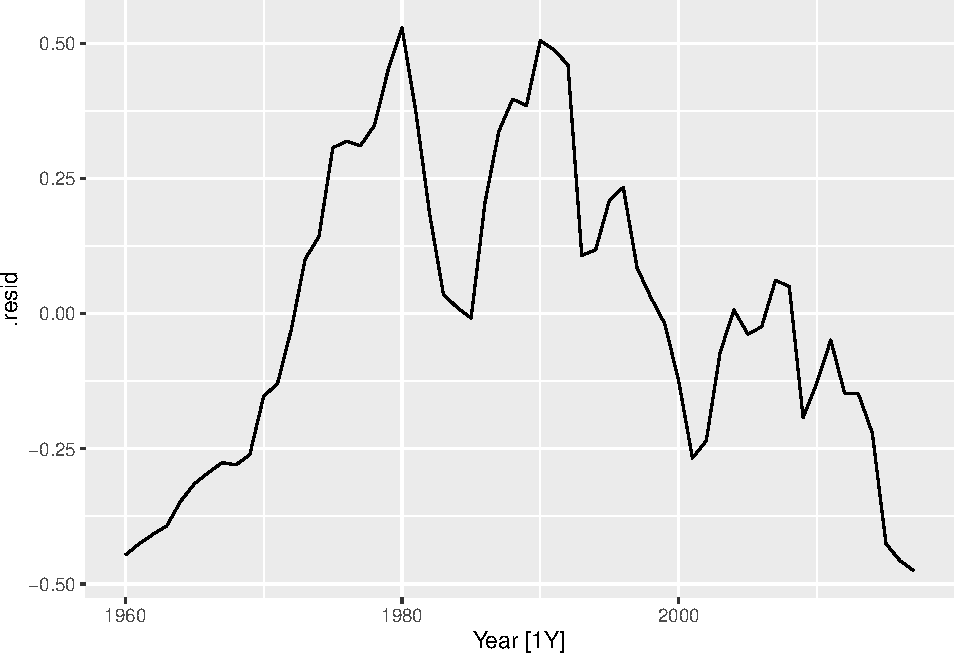
\includegraphics{graphics/unnamed-chunk-31-1.pdf}

\begin{Shaded}
\begin{Highlighting}[]
\NormalTok{global\_economy }\SpecialCharTok{\%\textgreater{}\%} \FunctionTok{model}\NormalTok{(}\AttributeTok{trend\_model =} \FunctionTok{TSLM}\NormalTok{(}\FunctionTok{log}\NormalTok{(GDP) }\SpecialCharTok{\textasciitilde{}} \FunctionTok{log}\NormalTok{(Population))) }\OtherTok{{-}\textgreater{}}\NormalTok{ fit3}

\NormalTok{fit3 }\SpecialCharTok{\%\textgreater{}\%} \FunctionTok{filter}\NormalTok{(Country }\SpecialCharTok{==} \StringTok{"Sweden"}\NormalTok{) }\SpecialCharTok{\%\textgreater{}\%} \FunctionTok{residuals}\NormalTok{() }\SpecialCharTok{\%\textgreater{}\%} \FunctionTok{autoplot}\NormalTok{()}
\end{Highlighting}
\end{Shaded}

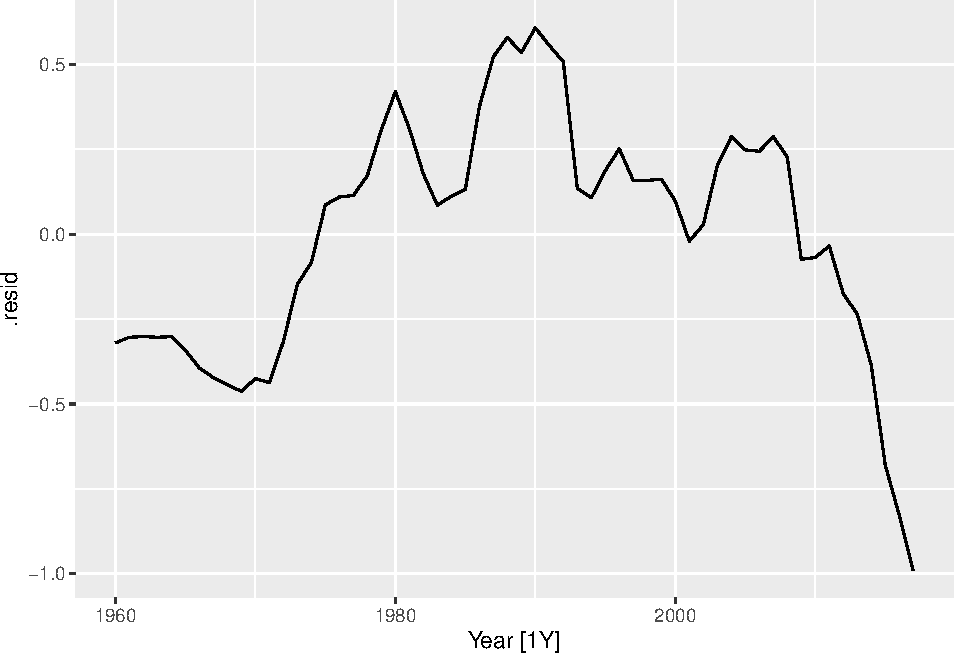
\includegraphics{graphics/unnamed-chunk-32-1.pdf}

\hypertarget{producing-forecasts}{%
\section{Producing forecasts}\label{producing-forecasts}}

\begin{Shaded}
\begin{Highlighting}[]
\NormalTok{fit }\SpecialCharTok{\%\textgreater{}\%} \FunctionTok{forecast}\NormalTok{(}\AttributeTok{h =} \StringTok{"3 years"}\NormalTok{) }\OtherTok{{-}\textgreater{}}\NormalTok{ fcast3yrs}

\NormalTok{fcast3yrs}
\end{Highlighting}
\end{Shaded}

\begin{verbatim}
## # A fable: 789 x 5 [1Y]
## # Key:     Country, .model [263]
##    Country        .model       Year                 GDP         .mean
##    <fct>          <chr>       <dbl>              <dist>         <dbl>
##  1 Afghanistan    trend_model  2018 N(1.6e+10, 1.3e+19)  16205101654.
##  2 Afghanistan    trend_model  2019 N(1.7e+10, 1.3e+19)  16511878141.
##  3 Afghanistan    trend_model  2020 N(1.7e+10, 1.3e+19)  16818654627.
##  4 Albania        trend_model  2018 N(1.4e+10, 3.9e+18)  13733734164.
##  5 Albania        trend_model  2019 N(1.4e+10, 3.9e+18)  14166852711.
##  6 Albania        trend_model  2020 N(1.5e+10, 3.9e+18)  14599971258.
##  7 Algeria        trend_model  2018 N(1.6e+11, 9.4e+20) 157895153441.
##  8 Algeria        trend_model  2019 N(1.6e+11, 9.4e+20) 161100952126.
##  9 Algeria        trend_model  2020 N(1.6e+11, 9.4e+20) 164306750811.
## 10 American Samoa trend_model  2018 N(6.8e+08, 1.7e+15)    682475000 
## # ... with 779 more rows
\end{verbatim}

\begin{Shaded}
\begin{Highlighting}[]
\NormalTok{fcast3yrs }\SpecialCharTok{\%\textgreater{}\%} \FunctionTok{filter}\NormalTok{(Country }\SpecialCharTok{==} \StringTok{"Sweden"}\NormalTok{, Year }\SpecialCharTok{==} \DecValTok{2020}\NormalTok{) }\SpecialCharTok{\%\textgreater{}\%} \FunctionTok{str}\NormalTok{()}
\end{Highlighting}
\end{Shaded}

\begin{verbatim}
## fbl_ts [1 x 5] (S3: fbl_ts/tbl_ts/tbl_df/tbl/data.frame)
##  $ Country: Factor w/ 263 levels "Afghanistan",..: 232
##  $ .model : chr "trend_model"
##  $ Year   : num 2020
##  $ GDP    : dist [1:1] 
##   ..$ 3:List of 2
##   .. ..$ mu   : num 5.45e+11
##   .. ..$ sigma: num 5.34e+10
##   .. ..- attr(*, "class")= chr [1:2] "dist_normal" "dist_default"
##   ..@ vars: chr "GDP"
##  $ .mean  : num 5.45e+11
##  - attr(*, "key")= tibble [1 x 3] (S3: tbl_df/tbl/data.frame)
##   ..$ Country: Factor w/ 263 levels "Afghanistan",..: 232
##   ..$ .model : chr "trend_model"
##   ..$ .rows  : list<int> [1:1] 
##   .. ..$ : int 1
##   .. ..@ ptype: int(0) 
##   ..- attr(*, ".drop")= logi TRUE
##  - attr(*, "index")= chr "Year"
##   ..- attr(*, "ordered")= logi TRUE
##  - attr(*, "index2")= chr "Year"
##  - attr(*, "interval")= interval [1:1] 1Y
##   ..@ .regular: logi TRUE
##  - attr(*, "response")= chr "GDP"
##  - attr(*, "dist")= chr "GDP"
##  - attr(*, "model_cn")= chr ".model"
\end{verbatim}

\begin{Shaded}
\begin{Highlighting}[]
\NormalTok{fcast3yrs }\SpecialCharTok{\%\textgreater{}\%}
  \FunctionTok{filter}\NormalTok{(Country}\SpecialCharTok{==}\StringTok{"Sweden"}\NormalTok{) }\SpecialCharTok{\%\textgreater{}\%}
  \FunctionTok{autoplot}\NormalTok{(global\_economy) }\SpecialCharTok{+}
  \FunctionTok{ggtitle}\NormalTok{(}\StringTok{"GDP for Sweden"}\NormalTok{) }\SpecialCharTok{+} \FunctionTok{ylab}\NormalTok{(}\StringTok{"$US billions"}\NormalTok{)}
\end{Highlighting}
\end{Shaded}

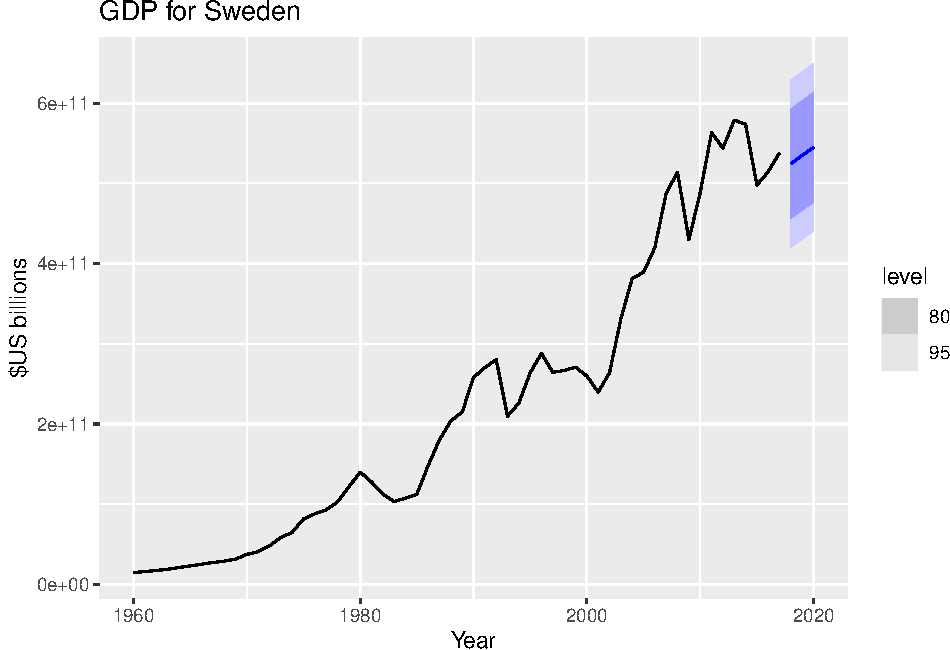
\includegraphics{graphics/visualize forecasts-1.pdf}

\hypertarget{model-residuals-vs.-forecast-errors}{%
\subsection{Model residuals vs.~forecast errors}\label{model-residuals-vs.-forecast-errors}}

Model residuals:

Your data: \(y_1, y_2, \ldots, y_T\)

Fitted values: \(\hat{y}_1, \hat{y}_2, \ldots, \hat{y}_T\)

Model residuals: \(e_t = y_t - \hat{y}_t\)

Forecast errors:

\begin{Shaded}
\begin{Highlighting}[]
\FunctionTok{augment}\NormalTok{(fit)}
\end{Highlighting}
\end{Shaded}

\begin{verbatim}
## # A tsibble: 15,150 x 7 [1Y]
## # Key:       Country, .model [263]
##    Country     .model       Year         GDP      .fitted      .resid     .innov
##    <fct>       <chr>       <dbl>       <dbl>        <dbl>       <dbl>      <dbl>
##  1 Afghanistan trend_model  1960  537777811. -1587934559. 2125712370.     2.13e9
##  2 Afghanistan trend_model  1961  548888896. -1281158073. 1830046968.     1.83e9
##  3 Afghanistan trend_model  1962  546666678.  -974381586. 1521048264.     1.52e9
##  4 Afghanistan trend_model  1963  751111191.  -667605100. 1418716291.     1.42e9
##  5 Afghanistan trend_model  1964  800000044.  -360828613. 1160828658.     1.16e9
##  6 Afghanistan trend_model  1965 1006666638.   -54052127. 1060718765.     1.06e9
##  7 Afghanistan trend_model  1966 1399999967.   252724359. 1147275607.     1.15e9
##  8 Afghanistan trend_model  1967 1673333418.   559500846. 1113832572.     1.11e9
##  9 Afghanistan trend_model  1968 1373333367.   866277332.  507056034.     5.07e8
## 10 Afghanistan trend_model  1969 1408888922.  1173053819.  235835103.     2.36e8
## # ... with 15,140 more rows
\end{verbatim}

\begin{Shaded}
\begin{Highlighting}[]
\FunctionTok{augment}\NormalTok{(fit) }\SpecialCharTok{\%\textgreater{}\%} \FunctionTok{filter}\NormalTok{(Country }\SpecialCharTok{==} \StringTok{"Sweden"}\NormalTok{) }\SpecialCharTok{\%\textgreater{}\%}
  \FunctionTok{ggplot}\NormalTok{(}\FunctionTok{aes}\NormalTok{(}\AttributeTok{x =}\NormalTok{ .resid)) }\SpecialCharTok{+}
  \FunctionTok{geom\_histogram}\NormalTok{(}\AttributeTok{bins =} \DecValTok{20}\NormalTok{) }\SpecialCharTok{+}
  \FunctionTok{ggtitle}\NormalTok{(}\StringTok{"Histogram of residuals"}\NormalTok{)}
\end{Highlighting}
\end{Shaded}

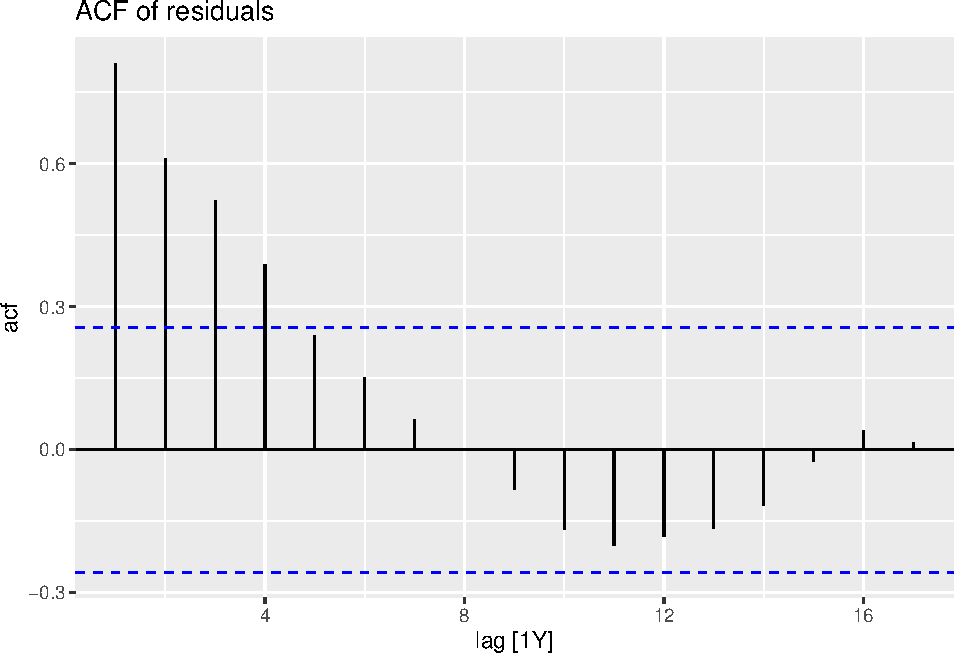
\includegraphics{graphics/unnamed-chunk-36-1.pdf}

\hypertarget{are-the-model-residuals-auto-correlated}{%
\subsection{Are the model residuals auto-correlated?}\label{are-the-model-residuals-auto-correlated}}

\begin{Shaded}
\begin{Highlighting}[]
\FunctionTok{augment}\NormalTok{(fit) }\SpecialCharTok{\%\textgreater{}\%} \FunctionTok{filter}\NormalTok{(Country }\SpecialCharTok{==} \StringTok{"Sweden"}\NormalTok{) }\OtherTok{{-}\textgreater{}}\NormalTok{ augSweden}

\NormalTok{augSweden }\SpecialCharTok{\%\textgreater{}\%}
  \FunctionTok{ACF}\NormalTok{(.resid) }\SpecialCharTok{\%\textgreater{}\%}
  \FunctionTok{autoplot}\NormalTok{() }\SpecialCharTok{+} \FunctionTok{ggtitle}\NormalTok{(}\StringTok{"ACF of residuals"}\NormalTok{)}
\end{Highlighting}
\end{Shaded}

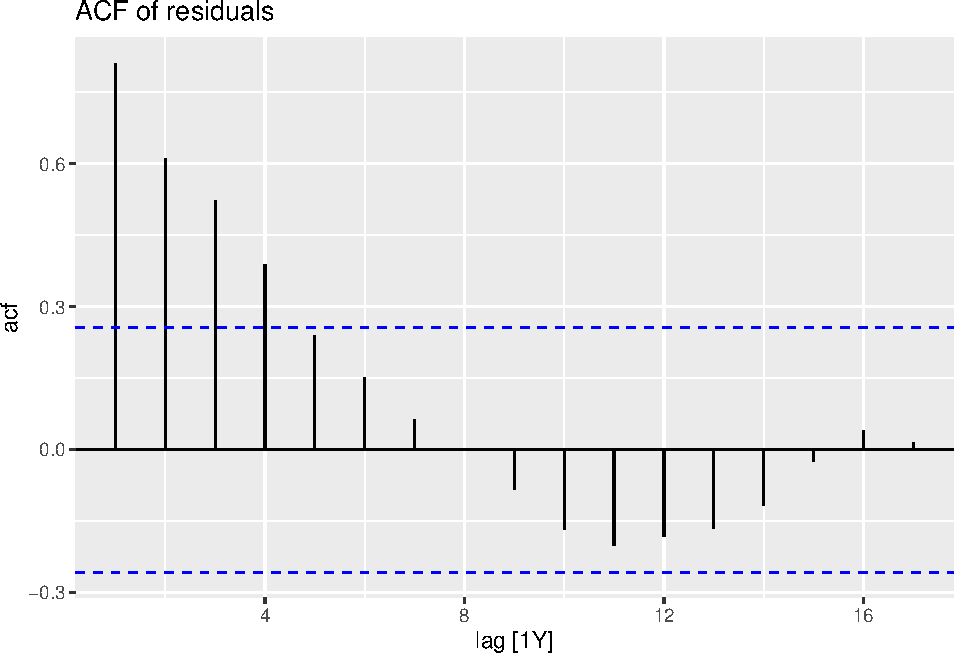
\includegraphics{graphics/unnamed-chunk-37-1.pdf}

\begin{Shaded}
\begin{Highlighting}[]
\FunctionTok{augment}\NormalTok{(fit3) }\SpecialCharTok{\%\textgreater{}\%} \FunctionTok{filter}\NormalTok{(Country }\SpecialCharTok{==} \StringTok{"Sweden"}\NormalTok{) }\OtherTok{{-}\textgreater{}}\NormalTok{ augSweden3}

\NormalTok{augSweden3 }\SpecialCharTok{\%\textgreater{}\%}
  \FunctionTok{ACF}\NormalTok{(.resid) }\SpecialCharTok{\%\textgreater{}\%}
  \FunctionTok{autoplot}\NormalTok{() }\SpecialCharTok{+} \FunctionTok{ggtitle}\NormalTok{(}\StringTok{"ACF of residuals"}\NormalTok{)}
\end{Highlighting}
\end{Shaded}

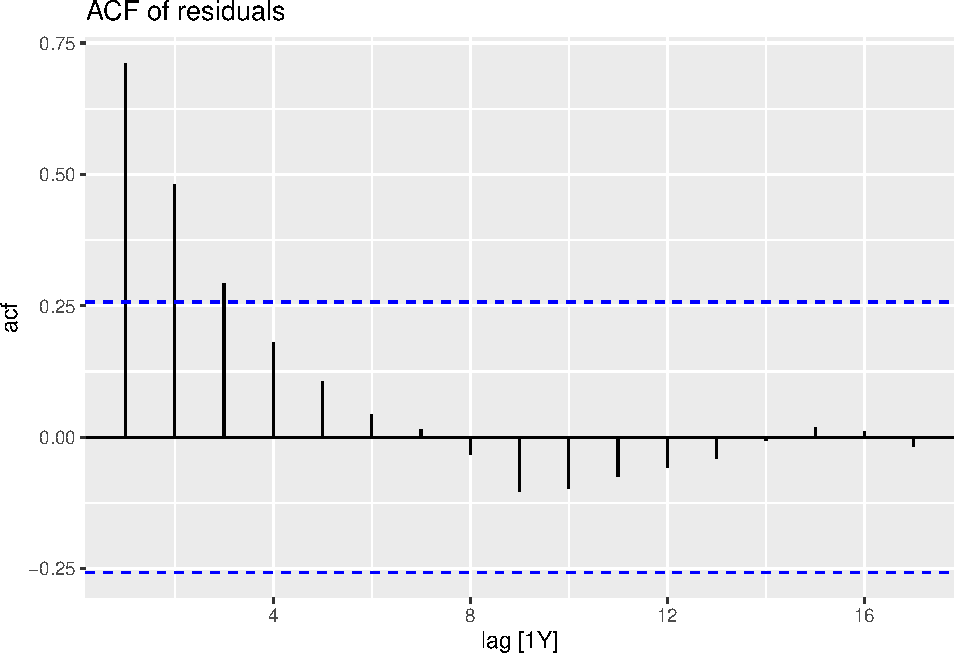
\includegraphics{graphics/unnamed-chunk-38-1.pdf}

\hypertarget{example-gdp-several-countries}{%
\section{Example: GDP, several countries}\label{example-gdp-several-countries}}

\begin{Shaded}
\begin{Highlighting}[]
\FunctionTok{library}\NormalTok{(tsibbledata) }\CommentTok{\# Data sets package}

\NormalTok{nordic }\OtherTok{\textless{}{-}} \FunctionTok{c}\NormalTok{(}\StringTok{"Sweden"}\NormalTok{, }\StringTok{"Denmark"}\NormalTok{, }\StringTok{"Norway"}\NormalTok{, }\StringTok{"Finland"}\NormalTok{)}

\NormalTok{(global\_economy }\SpecialCharTok{\%\textgreater{}\%} \FunctionTok{filter}\NormalTok{(Country }\SpecialCharTok{\%in\%}\NormalTok{ nordic) }\OtherTok{{-}\textgreater{}}\NormalTok{ nordic\_economy)}
\end{Highlighting}
\end{Shaded}

\begin{verbatim}
## # A tsibble: 232 x 9 [1Y]
## # Key:       Country [4]
##    Country Code   Year          GDP Growth   CPI Imports Exports Population
##    <fct>   <fct> <dbl>        <dbl>  <dbl> <dbl>   <dbl>   <dbl>      <dbl>
##  1 Denmark DNK    1960  6248946880. NA      8.25    34.3    32.3    4579603
##  2 Denmark DNK    1961  6933842099.  6.38   8.53    32.3    30.0    4611687
##  3 Denmark DNK    1962  7812968114.  5.67   9.16    32.5    28.6    4647727
##  4 Denmark DNK    1963  8316692386.  0.637  9.72    30.8    30.4    4684483
##  5 Denmark DNK    1964  9506678763.  9.27  10.0     32.6    29.9    4722072
##  6 Denmark DNK    1965 10678897387.  4.56  10.6     31.5    29.3    4759012
##  7 Denmark DNK    1966 11721248101.  2.74  11.3     30.8    28.6    4797381
##  8 Denmark DNK    1967 12788479692.  3.42  12.2     30.0    27.3    4835354
##  9 Denmark DNK    1968 13196541952   3.97  13.2     29.7    27.7    4864883
## 10 Denmark DNK    1969 15009384585.  6.32  13.7     30.4    27.6    4891860
## # ... with 222 more rows
\end{verbatim}

\begin{Shaded}
\begin{Highlighting}[]
\NormalTok{nordic\_economy }\SpecialCharTok{\%\textgreater{}\%} \FunctionTok{autoplot}\NormalTok{(GDP)}
\end{Highlighting}
\end{Shaded}

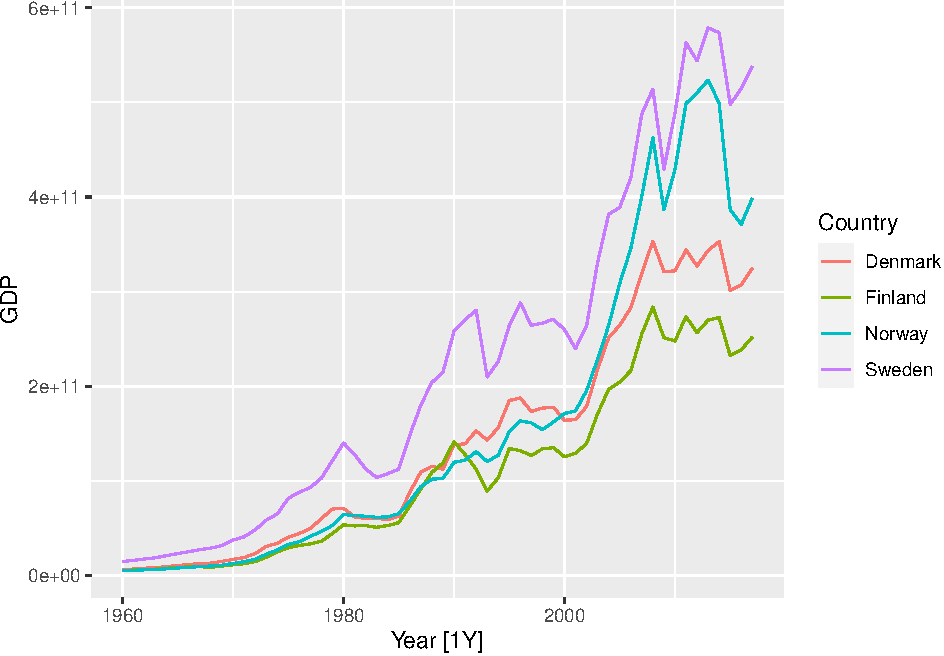
\includegraphics{graphics/unnamed-chunk-40-1.pdf}

\begin{Shaded}
\begin{Highlighting}[]
\NormalTok{fitnord }\OtherTok{\textless{}{-}}\NormalTok{ nordic\_economy }\SpecialCharTok{\%\textgreater{}\%}
  \FunctionTok{model}\NormalTok{(}
    \AttributeTok{trend\_model =} \FunctionTok{TSLM}\NormalTok{(GDP }\SpecialCharTok{\textasciitilde{}} \FunctionTok{trend}\NormalTok{()),}
    \AttributeTok{trend\_model\_ln =} \FunctionTok{TSLM}\NormalTok{(}\FunctionTok{log}\NormalTok{(GDP) }\SpecialCharTok{\textasciitilde{}} \FunctionTok{trend}\NormalTok{()),}
    \AttributeTok{ets =} \FunctionTok{ETS}\NormalTok{(GDP }\SpecialCharTok{\textasciitilde{}} \FunctionTok{trend}\NormalTok{(}\StringTok{"A"}\NormalTok{)),}
    \AttributeTok{arima =} \FunctionTok{ARIMA}\NormalTok{(GDP)}
\NormalTok{  )}

\NormalTok{fitnord}
\end{Highlighting}
\end{Shaded}

\begin{verbatim}
## # A mable: 4 x 5
## # Key:     Country [4]
##   Country trend_model trend_model_ln          ets          arima
##   <fct>       <model>        <model>      <model>        <model>
## 1 Denmark      <TSLM>         <TSLM> <ETS(M,A,N)> <ARIMA(1,1,1)>
## 2 Finland      <TSLM>         <TSLM> <ETS(M,A,N)> <ARIMA(0,1,2)>
## 3 Norway       <TSLM>         <TSLM> <ETS(M,A,N)> <ARIMA(0,1,1)>
## 4 Sweden       <TSLM>         <TSLM> <ETS(M,A,N)> <ARIMA(0,1,2)>
\end{verbatim}

\begin{Shaded}
\begin{Highlighting}[]
\NormalTok{fitnord }\SpecialCharTok{\%\textgreater{}\%}
\NormalTok{  dplyr}\SpecialCharTok{::}\FunctionTok{select}\NormalTok{(arima) }\SpecialCharTok{\%\textgreater{}\%}
  \FunctionTok{coef}\NormalTok{()}
\end{Highlighting}
\end{Shaded}

\begin{verbatim}
## # A tibble: 7 x 7
##   Country .model term  estimate std.error statistic    p.value
##   <fct>   <chr>  <chr>    <dbl>     <dbl>     <dbl>      <dbl>
## 1 Denmark arima  ar1     -0.390     0.206     -1.89 0.0636    
## 2 Denmark arima  ma1      0.724     0.143      5.05 0.00000484
## 3 Finland arima  ma1      0.406     0.120      3.39 0.00126   
## 4 Finland arima  ma2     -0.221     0.108     -2.05 0.0450    
## 5 Norway  arima  ma1      0.410     0.155      2.65 0.0104    
## 6 Sweden  arima  ma1      0.241     0.121      1.99 0.0510    
## 7 Sweden  arima  ma2     -0.188     0.101     -1.87 0.0670
\end{verbatim}

Denmark: ARMA(1,1)

Finland: MA(2)

Norway: MA(1)

Sweden: MA(2)

\begin{Shaded}
\begin{Highlighting}[]
\NormalTok{nordic\_economy }\SpecialCharTok{\%\textgreater{}\%}
  \FunctionTok{model}\NormalTok{(}\AttributeTok{arima\_constrained =} \FunctionTok{ARIMA}\NormalTok{(GDP }\SpecialCharTok{\textasciitilde{}} \FunctionTok{pdq}\NormalTok{(}\DecValTok{1}\NormalTok{,}\DecValTok{0}\NormalTok{,}\DecValTok{2}\NormalTok{))) }\SpecialCharTok{\%\textgreater{}\%}\NormalTok{ dplyr}\SpecialCharTok{::}\FunctionTok{select}\NormalTok{(arima\_constrained) }\SpecialCharTok{\%\textgreater{}\%} \FunctionTok{coef}\NormalTok{()}
\end{Highlighting}
\end{Shaded}

\begin{verbatim}
## # A tibble: 0 x 4
## # ... with 4 variables: Country <fct>, .model <chr>, term <chr>, estimate <dbl>
\end{verbatim}

\begin{Shaded}
\begin{Highlighting}[]
\NormalTok{fitnord }\SpecialCharTok{\%\textgreater{}\%} \FunctionTok{coef}\NormalTok{()}
\end{Highlighting}
\end{Shaded}

\begin{verbatim}
## # A tibble: 39 x 7
##    Country .model         term         estimate std.error statistic   p.value
##    <fct>   <chr>          <chr>           <dbl>     <dbl>     <dbl>     <dbl>
##  1 Denmark trend_model    (Intercept) -5.65e+10   8.75e+9     -6.46  2.70e- 8
##  2 Denmark trend_model    trend()      6.63e+ 9   2.58e+8     25.7   1.14e-32
##  3 Denmark trend_model_ln (Intercept)  2.30e+ 1   8.55e-2    269.    7.68e-89
##  4 Denmark trend_model_ln trend()      7.12e- 2   2.52e-3     28.3   7.68e-35
##  5 Denmark ets            alpha        1.00e+ 0  NA           NA    NA       
##  6 Denmark ets            beta         3.67e- 1  NA           NA    NA       
##  7 Denmark ets            l[0]         4.92e+ 9  NA           NA    NA       
##  8 Denmark ets            b[0]         1.24e+ 9  NA           NA    NA       
##  9 Denmark arima          ar1         -3.90e- 1   2.06e-1     -1.89  6.36e- 2
## 10 Denmark arima          ma1          7.24e- 1   1.43e-1      5.05  4.84e- 6
## # ... with 29 more rows
\end{verbatim}

\begin{Shaded}
\begin{Highlighting}[]
\NormalTok{fitnord }\SpecialCharTok{\%\textgreater{}\%}  \FunctionTok{glance}\NormalTok{()  }
\end{Highlighting}
\end{Shaded}

\begin{verbatim}
## # A tibble: 16 x 21
##    Country .model     r_squared adj_r_squared   sigma2 statistic   p_value    df
##    <fct>   <chr>          <dbl>         <dbl>    <dbl>     <dbl>     <dbl> <int>
##  1 Denmark trend_mod~     0.922         0.920 1.08e+21      660.  1.14e-32     2
##  2 Denmark trend_mod~     0.935         0.933 1.03e- 1      800.  7.68e-35     2
##  3 Denmark ets           NA            NA     1.04e- 2       NA  NA           NA
##  4 Denmark arima         NA            NA     2.41e+20       NA  NA           NA
##  5 Finland trend_mod~     0.914         0.912 7.34e+20      594.  1.70e-31     2
##  6 Finland trend_mod~     0.930         0.929 1.14e- 1      745.  4.96e-34     2
##  7 Finland ets           NA            NA     1.32e- 2       NA  NA           NA
##  8 Finland arima         NA            NA     1.89e+20       NA  NA           NA
##  9 Norway  trend_mod~     0.824         0.821 4.60e+21      262.  8.54e-23     2
## 10 Norway  trend_mod~     0.959         0.958 8.37e- 2     1307.  1.64e-40     2
## 11 Norway  ets           NA            NA     8.23e- 3       NA  NA           NA
## 12 Norway  arima         NA            NA     6.78e+20       NA  NA           NA
## 13 Sweden  trend_mod~     0.919         0.918 2.65e+21      635.  3.07e-32     2
## 14 Sweden  trend_mod~     0.935         0.933 8.19e- 2      800.  7.57e-35     2
## 15 Sweden  ets           NA            NA     1.16e- 2       NA  NA           NA
## 16 Sweden  arima         NA            NA     8.84e+20       NA  NA           NA
## # ... with 13 more variables: log_lik <dbl>, AIC <dbl>, AICc <dbl>, BIC <dbl>,
## #   CV <dbl>, deviance <dbl>, df.residual <int>, rank <int>, MSE <dbl>,
## #   AMSE <dbl>, MAE <dbl>, ar_roots <list>, ma_roots <list>
\end{verbatim}

\begin{Shaded}
\begin{Highlighting}[]
\NormalTok{fitnord }\SpecialCharTok{\%\textgreater{}\%} \FunctionTok{filter}\NormalTok{(Country }\SpecialCharTok{==} \StringTok{"Denmark"}\NormalTok{) }\SpecialCharTok{\%\textgreater{}\%}\NormalTok{ dplyr}\SpecialCharTok{::}\FunctionTok{select}\NormalTok{(arima) }\SpecialCharTok{\%\textgreater{}\%} \FunctionTok{report}\NormalTok{()}
\end{Highlighting}
\end{Shaded}

\begin{verbatim}
## Series: GDP 
## Model: ARIMA(1,1,1) 
## 
## Coefficients:
##           ar1     ma1
##       -0.3898  0.7240
## s.e.   0.2061  0.1434
## 
## sigma^2 estimated as 2.407e+20:  log likelihood=-1417.5
## AIC=2840.99   AICc=2841.45   BIC=2847.12
\end{verbatim}

\begin{Shaded}
\begin{Highlighting}[]
\NormalTok{fitnord }\SpecialCharTok{\%\textgreater{}\%}
  \FunctionTok{accuracy}\NormalTok{() }\SpecialCharTok{\%\textgreater{}\%}
  \FunctionTok{arrange}\NormalTok{(Country, MPE)}
\end{Highlighting}
\end{Shaded}

\begin{verbatim}
## # A tibble: 16 x 11
##    Country .model     .type        ME    RMSE     MAE     MPE   MAPE  MASE RMSSE
##    <fct>   <chr>      <chr>     <dbl>   <dbl>   <dbl>   <dbl>  <dbl> <dbl> <dbl>
##  1 Denmark trend_mod~ Trai~ -1.12e+10 6.89e10 3.67e10  -5.17   28.0  3.34  4.24 
##  2 Denmark ets        Trai~  4.50e+ 7 1.65e10 1.04e10   0.518   7.09 0.946 1.02 
##  3 Denmark arima      Trai~  4.40e+ 9 1.51e10 1.04e10   5.05    8.16 0.945 0.930
##  4 Denmark trend_mod~ Trai~ -2.06e- 6 3.23e10 2.63e10  51.1    80.8  2.40  1.99 
##  5 Finland trend_mod~ Trai~ -8.61e+ 9 5.64e10 2.99e10  -5.53   28.6  2.95  3.82 
##  6 Finland ets        Trai~  1.36e+ 8 1.47e10 9.41e 9   0.795   8.36 0.927 0.996
##  7 Finland arima      Trai~  3.54e+ 9 1.34e10 9.14e 9   5.03    8.92 0.900 0.906
##  8 Finland trend_mod~ Trai~  9.54e- 7 2.66e10 2.21e10  46.1    80.5  2.18  1.80 
##  9 Norway  trend_mod~ Trai~ -1.31e+10 8.20e10 3.51e10  -4.24   24.9  2.24  3.01 
## 10 Norway  ets        Trai~ -5.29e+ 8 2.75e10 1.37e10   0.755   6.94 0.870 1.01 
## 11 Norway  arima      Trai~  4.90e+ 9 2.56e10 1.40e10   5.04    8.11 0.890 0.938
## 12 Norway  trend_mod~ Trai~  2.09e- 6 6.67e10 5.48e10 130.    181.   3.49  2.45 
## 13 Sweden  trend_mod~ Trai~ -1.18e+10 8.23e10 4.79e10  -3.96   23.7  2.25  2.68 
## 14 Sweden  ets        Trai~  1.19e+ 9 3.02e10 1.86e10   0.745   7.64 0.875 0.984
## 15 Sweden  arima      Trai~  8.48e+ 9 2.89e10 2.01e10   5.18    9.37 0.942 0.944
## 16 Sweden  trend_mod~ Trai~  2.10e- 6 5.05e10 3.90e10  29.4    53.3  1.83  1.65 
## # ... with 1 more variable: ACF1 <dbl>
\end{verbatim}

\begin{Shaded}
\begin{Highlighting}[]
\CommentTok{\# ETS forecasts}
\NormalTok{USAccDeaths }\SpecialCharTok{\%\textgreater{}\%}
  \FunctionTok{ets}\NormalTok{() }\SpecialCharTok{\%\textgreater{}\%}
  \FunctionTok{forecast}\NormalTok{() }\SpecialCharTok{\%\textgreater{}\%}
  \FunctionTok{autoplot}\NormalTok{()}
\end{Highlighting}
\end{Shaded}

\begin{Shaded}
\begin{Highlighting}[]
\FunctionTok{str}\NormalTok{(taylor)}
\FunctionTok{plot}\NormalTok{(taylor)}
\end{Highlighting}
\end{Shaded}

\hypertarget{plot-lagged-values}{%
\subsection{Plot lagged values}\label{plot-lagged-values}}

\begin{Shaded}
\begin{Highlighting}[]
\NormalTok{vaelsales\_tbl\_ts  }\SpecialCharTok{\%\textgreater{}\%} \FunctionTok{filter}\NormalTok{(}\FunctionTok{month}\NormalTok{(Month) }\SpecialCharTok{\%in\%} \FunctionTok{c}\NormalTok{(}\DecValTok{3}\NormalTok{,}\DecValTok{6}\NormalTok{,}\DecValTok{9}\NormalTok{,}\DecValTok{12}\NormalTok{)) }\SpecialCharTok{\%\textgreater{}\%} \FunctionTok{gg\_lag}\NormalTok{(sales\_GWh, }\AttributeTok{lags =} \DecValTok{1}\SpecialCharTok{:}\DecValTok{2}\NormalTok{)}
\end{Highlighting}
\end{Shaded}

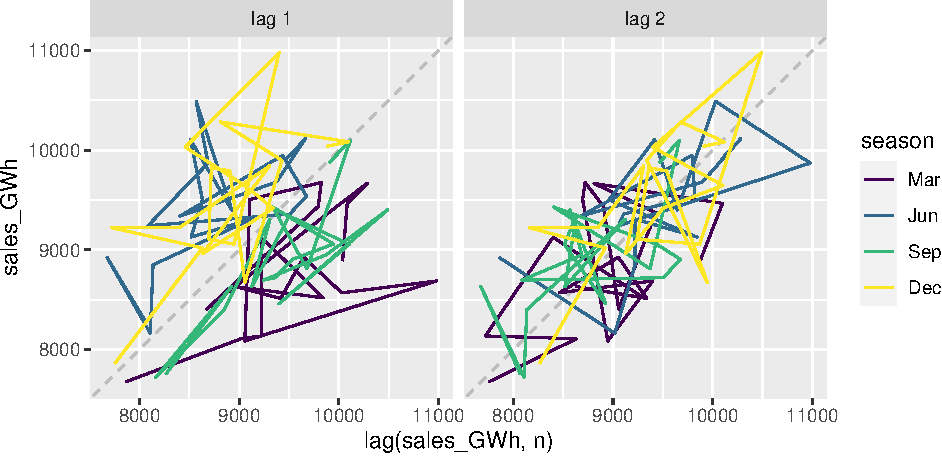
\includegraphics{graphics/plot lagged values-1.pdf}

\begin{Shaded}
\begin{Highlighting}[]
\NormalTok{vaelsales\_tbl\_ts  }\SpecialCharTok{\%\textgreater{}\%} \FunctionTok{filter}\NormalTok{(}\FunctionTok{month}\NormalTok{(Month) }\SpecialCharTok{==} \DecValTok{1}\NormalTok{) }\SpecialCharTok{\%\textgreater{}\%} \FunctionTok{gg\_lag}\NormalTok{(sales\_GWh, }\AttributeTok{lags =} \DecValTok{1}\SpecialCharTok{:}\DecValTok{2}\NormalTok{)}
\end{Highlighting}
\end{Shaded}

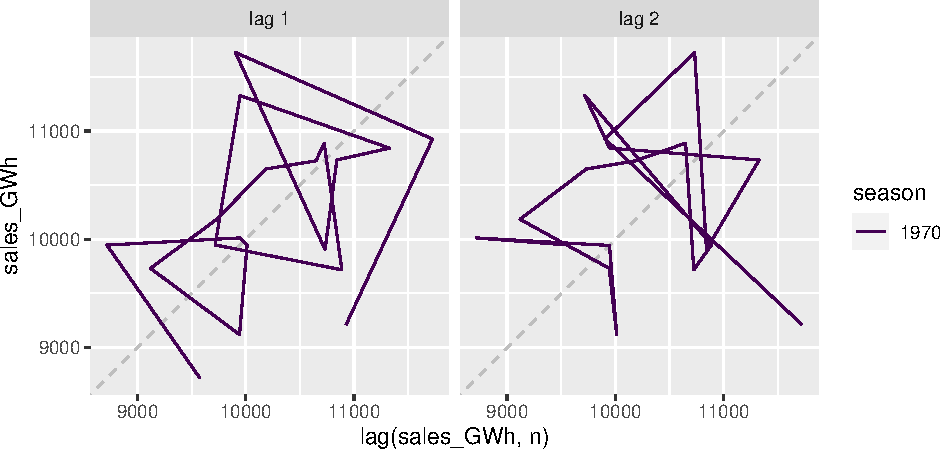
\includegraphics{graphics/plot lagged values-2.pdf}

\begin{Shaded}
\begin{Highlighting}[]
\NormalTok{vaelsales\_tbl\_ts }\SpecialCharTok{\%\textgreater{}\%} \FunctionTok{ACF}\NormalTok{(sales\_GWh) }\SpecialCharTok{\%\textgreater{}\%} \FunctionTok{autoplot}\NormalTok{()}
\end{Highlighting}
\end{Shaded}

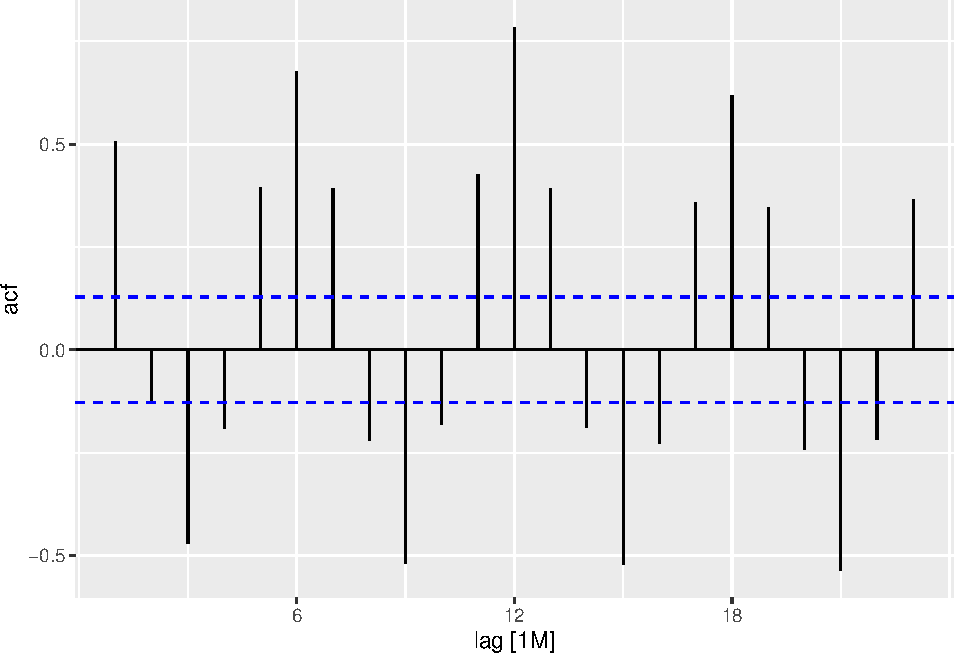
\includegraphics{graphics/unnamed-chunk-50-1.pdf}

\begin{Shaded}
\begin{Highlighting}[]
\CommentTok{\# decompose(vaelsales\_tbl\_ts)}
\end{Highlighting}
\end{Shaded}

\begin{Shaded}
\begin{Highlighting}[]
\NormalTok{vaelsales\_tbl\_ts }\SpecialCharTok{\%\textgreater{}\%}
  \FunctionTok{model}\NormalTok{(}\FunctionTok{STL}\NormalTok{(sales\_GWh }\SpecialCharTok{\textasciitilde{}} \FunctionTok{trend}\NormalTok{(}\AttributeTok{window=}\DecValTok{21}\NormalTok{) }\SpecialCharTok{+} \FunctionTok{season}\NormalTok{(}\AttributeTok{window=}\StringTok{\textquotesingle{}periodic\textquotesingle{}}\NormalTok{), }\AttributeTok{robust =} \ConstantTok{TRUE}\NormalTok{)) }\SpecialCharTok{\%\textgreater{}\%}
  \FunctionTok{components}\NormalTok{() }\SpecialCharTok{\%\textgreater{}\%}
  \FunctionTok{autoplot}\NormalTok{()}
\end{Highlighting}
\end{Shaded}

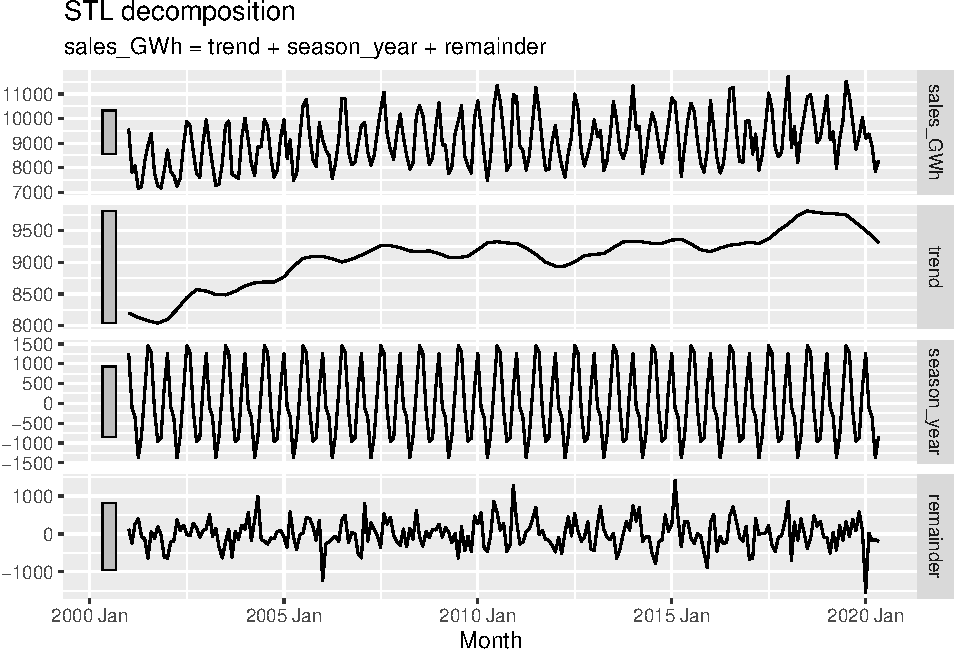
\includegraphics{graphics/perform additive STL decomposition of the VA electricity sales time series-1.pdf}

\begin{Shaded}
\begin{Highlighting}[]
\NormalTok{vaelsales\_tbl\_ts }\SpecialCharTok{\%\textgreater{}\%}
  \FunctionTok{mutate}\NormalTok{(}\AttributeTok{ln\_sales\_GWh =} \FunctionTok{log}\NormalTok{(sales\_GWh)) }\SpecialCharTok{\%\textgreater{}\%}
  \FunctionTok{model}\NormalTok{(}\FunctionTok{STL}\NormalTok{(ln\_sales\_GWh }\SpecialCharTok{\textasciitilde{}} \FunctionTok{trend}\NormalTok{(}\AttributeTok{window=}\DecValTok{21}\NormalTok{) }\SpecialCharTok{+} \FunctionTok{season}\NormalTok{(}\AttributeTok{window=}\StringTok{\textquotesingle{}periodic\textquotesingle{}}\NormalTok{),}
    \AttributeTok{robust =} \ConstantTok{TRUE}\NormalTok{)) }\SpecialCharTok{\%\textgreater{}\%}
  \FunctionTok{components}\NormalTok{() }\SpecialCharTok{\%\textgreater{}\%}
  \FunctionTok{autoplot}\NormalTok{()}
\end{Highlighting}
\end{Shaded}

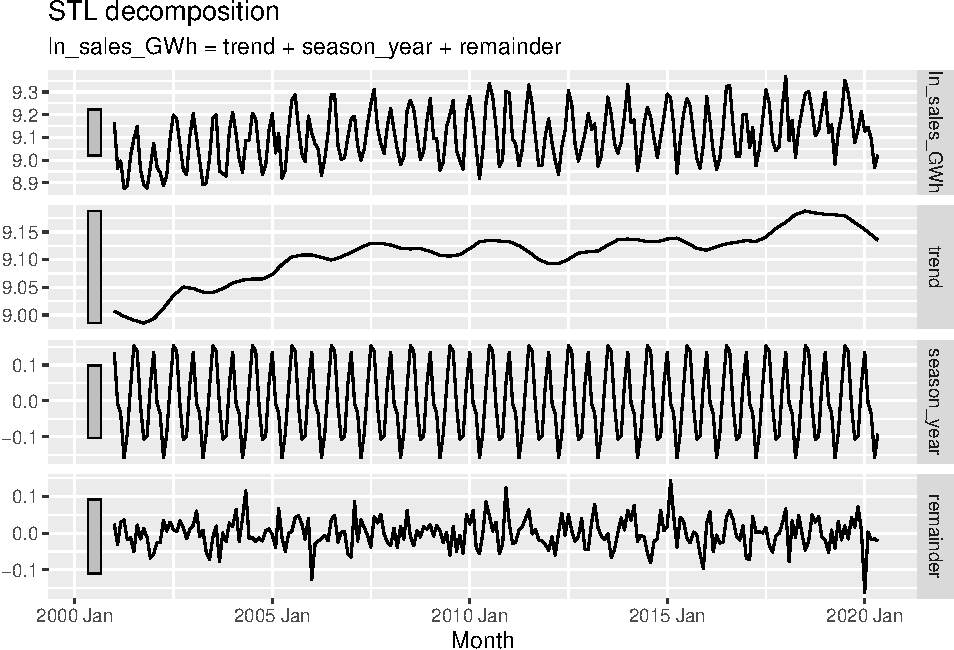
\includegraphics{graphics/perform multiplicative STL decomposition of the VA electricity sales time series-1.pdf}

\begin{Shaded}
\begin{Highlighting}[]
\NormalTok{vaelsales\_tbl\_ts }\SpecialCharTok{\%\textgreater{}\%}
  \FunctionTok{features}\NormalTok{(sales\_GWh, feat\_stl)}
\end{Highlighting}
\end{Shaded}

\begin{verbatim}
## # A tibble: 1 x 9
##   trend_strength seasonal_strength_~ seasonal_peak_y~ seasonal_trough~ spikiness
##            <dbl>               <dbl>            <dbl>            <dbl>     <dbl>
## 1          0.609               0.869                7                4   747395.
## # ... with 4 more variables: linearity <dbl>, curvature <dbl>,
## #   stl_e_acf1 <dbl>, stl_e_acf10 <dbl>
\end{verbatim}

\begin{Shaded}
\begin{Highlighting}[]
\NormalTok{vaelsales\_tbl\_ts }\SpecialCharTok{\%\textgreater{}\%}
  \FunctionTok{features}\NormalTok{(sales\_GWh, }\FunctionTok{feature\_set}\NormalTok{(}\AttributeTok{pkgs=}\StringTok{"feasts"}\NormalTok{))}
\end{Highlighting}
\end{Shaded}

\begin{verbatim}
## # A tibble: 1 x 47
##   trend_strength seasonal_strength_~ seasonal_peak_y~ seasonal_trough~ spikiness
##            <dbl>               <dbl>            <dbl>            <dbl>     <dbl>
## 1          0.609               0.869                7                4   747395.
## # ... with 42 more variables: linearity <dbl>, curvature <dbl>,
## #   stl_e_acf1 <dbl>, stl_e_acf10 <dbl>, acf1 <dbl>, acf10 <dbl>,
## #   diff1_acf1 <dbl>, diff1_acf10 <dbl>, diff2_acf1 <dbl>, diff2_acf10 <dbl>,
## #   season_acf1 <dbl>, pacf5 <dbl>, diff1_pacf5 <dbl>, diff2_pacf5 <dbl>,
## #   season_pacf <dbl>, zero_run_mean <dbl>, nonzero_squared_cv <dbl>,
## #   zero_start_prop <dbl>, zero_end_prop <dbl>, lambda_guerrero <dbl>,
## #   kpss_stat <dbl>, kpss_pvalue <dbl>, pp_stat <dbl>, pp_pvalue <dbl>, ...
\end{verbatim}

\hypertarget{autocorrelation}{%
\chapter{Autocorrelation}\label{autocorrelation}}

Readings: FPP3 Sections 2.7-2.9, 4.2, 4.5

\begin{Shaded}
\begin{Highlighting}[]
\NormalTok{vaelsales\_tbl\_ts  }\SpecialCharTok{\%\textgreater{}\%} \FunctionTok{filter}\NormalTok{(}\FunctionTok{month}\NormalTok{(Month) }\SpecialCharTok{\%in\%} \FunctionTok{c}\NormalTok{(}\DecValTok{3}\NormalTok{,}\DecValTok{6}\NormalTok{,}\DecValTok{9}\NormalTok{,}\DecValTok{12}\NormalTok{)) }\SpecialCharTok{\%\textgreater{}\%} \FunctionTok{gg\_lag}\NormalTok{(sales\_GWh, }\AttributeTok{lags =} \DecValTok{1}\SpecialCharTok{:}\DecValTok{2}\NormalTok{)}
\end{Highlighting}
\end{Shaded}

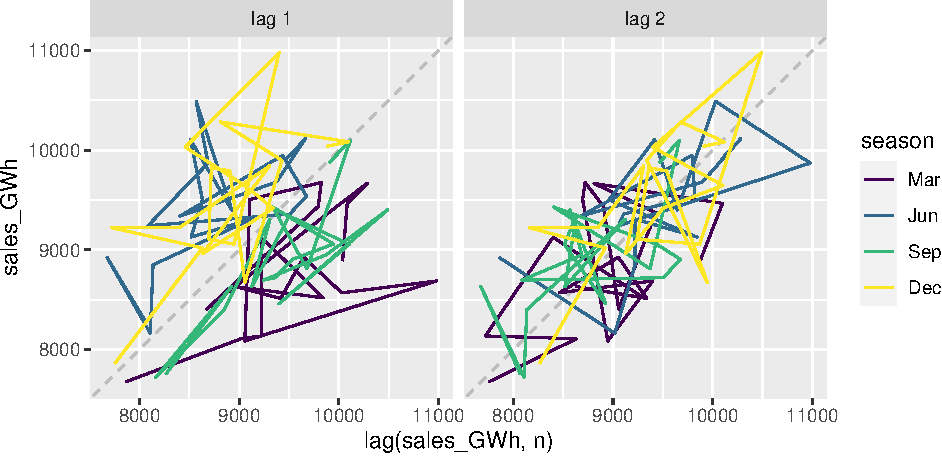
\includegraphics{graphics/plot lagged values 2-1.pdf}

\begin{Shaded}
\begin{Highlighting}[]
\NormalTok{vaelsales\_tbl\_ts  }\SpecialCharTok{\%\textgreater{}\%} \FunctionTok{filter}\NormalTok{(}\FunctionTok{month}\NormalTok{(Month) }\SpecialCharTok{==} \DecValTok{1}\NormalTok{) }\SpecialCharTok{\%\textgreater{}\%} \FunctionTok{gg\_lag}\NormalTok{(sales\_GWh, }\AttributeTok{lags =} \DecValTok{1}\SpecialCharTok{:}\DecValTok{2}\NormalTok{)}
\end{Highlighting}
\end{Shaded}

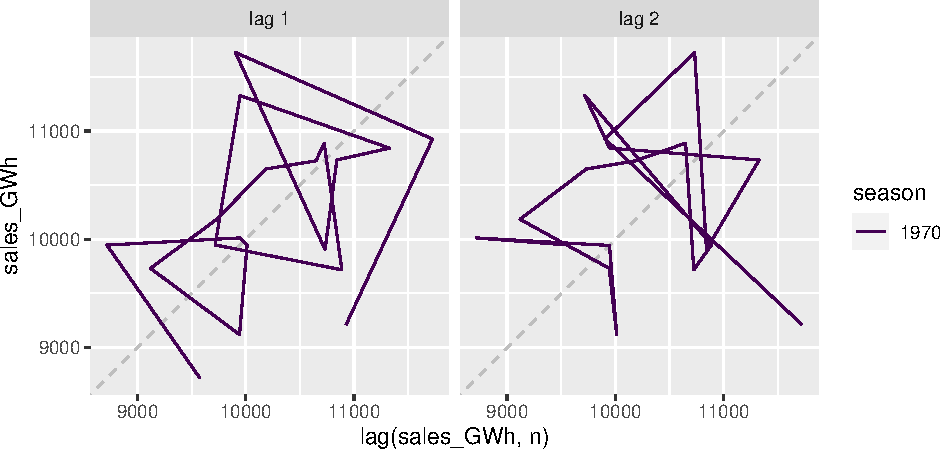
\includegraphics{graphics/plot lagged values 2-2.pdf}

\begin{Shaded}
\begin{Highlighting}[]
\NormalTok{vaelsales\_tbl\_ts }\SpecialCharTok{\%\textgreater{}\%} \FunctionTok{ACF}\NormalTok{(sales\_GWh) }\SpecialCharTok{\%\textgreater{}\%} \FunctionTok{autoplot}\NormalTok{()}
\end{Highlighting}
\end{Shaded}

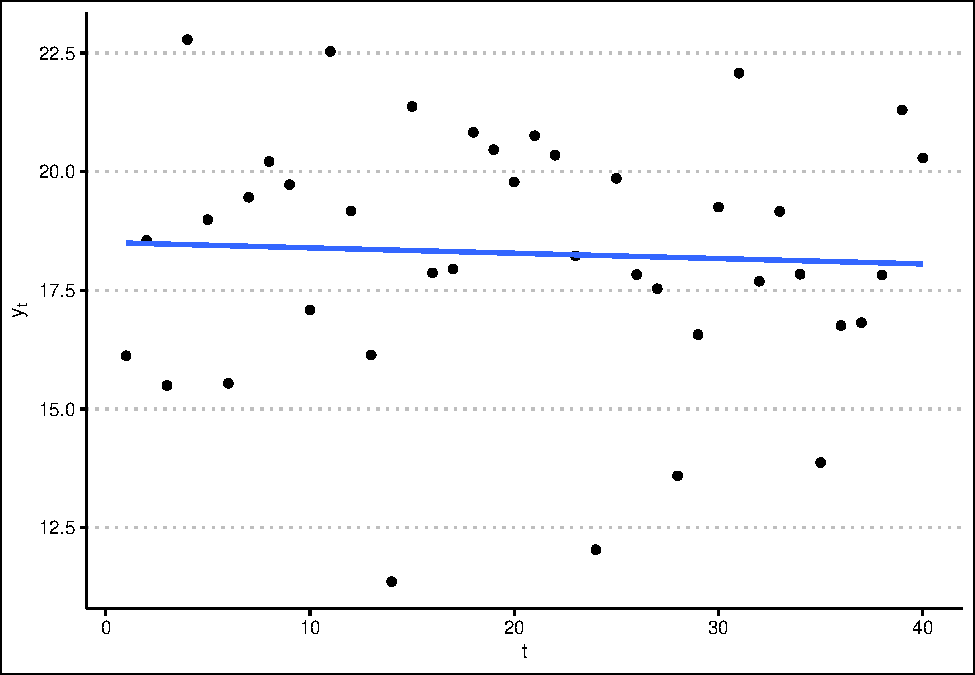
\includegraphics{graphics/unnamed-chunk-55-1.pdf}

\hypertarget{heere-be-monsters}{%
\section{Heere be monsters}\label{heere-be-monsters}}

\begin{Shaded}
\begin{Highlighting}[]
\NormalTok{knitr}\SpecialCharTok{::}\FunctionTok{include\_graphics}\NormalTok{(}\StringTok{"graphics/horst\_acf/horst\_acf\_1.jpg"}\NormalTok{)}
\end{Highlighting}
\end{Shaded}

\includegraphics{graphics/horst_acf/horst_acf_1.jpg}

\hypertarget{part-model-specification-and-estimation}{%
\part{Model Specification and Estimation}\label{part-model-specification-and-estimation}}

\hypertarget{the-data-generating-process}{%
\chapter{The data-generating process}\label{the-data-generating-process}}

In Section \ref{ts-table} we introduced a structure for a typical table of time series data:

\begin{longtable}[]{@{}ccccc@{}}
\toprule
Date & Series & Value\_1 & Value\_2 & Value\_3 \\
\midrule
\endhead
2020-02-01 & ``Virginia'' & 33.57 & 29 & ``friendly'' \\
2020-02-01 & ``Idaho'' & 0.22 & 18 & ``hostile'' \\
\ldots{} & \ldots{} & \ldots{} & \ldots{} & \ldots{} \\
\texttt{index} & \texttt{key} & & & \\
{[}date{]} & {[}fctr{]} & {[}dbl{]} & {[}int{]} & {[}fctr{]} \\
\bottomrule
\end{longtable}

Here, the \texttt{Date} field contains values for regular time intervals on which data are recorded. The fields \texttt{Value\_1}, \texttt{Value\_2}, etc., contain the actual observed values. The \texttt{Series} field reports objects (here, U.S. states) for which data are reported.

Let's make this setup both simpler and somewhat more general. For now, let's drop the key field \texttt{Series}, and suppose we are dealing only with one time series. Let's abstract from the \texttt{Date} field, and just label the sequence of time steps \(t = 1,2,\ldots,T\). Let's suppose further we have only one sequence of data values \(y_1, y_2, \ldots, y_T\). Our abstracted data table now looks like:

\begin{longtable}[]{@{}cc@{}}
\toprule
\(t\) & \(y\) \\
\midrule
\endhead
\(1\) & \(y_1\) \\
\(2\) & \(y_2\) \\
\ldots{} & \ldots{} \\
\(T\) & \(y_T\) \\
\bottomrule
\end{longtable}

Suppose we have a dataset structured in this way:

\begin{verbatim}
## # A tibble: 40 x 2
##        t     y
##    <int> <dbl>
##  1     1  16.1
##  2     2  18.6
##  3     3  15.5
##  4     4  22.8
##  5     5  19.0
##  6     6  15.5
##  7     7  19.5
##  8     8  20.2
##  9     9  19.7
## 10    10  17.1
## # ... with 30 more rows
\end{verbatim}

Given such a dataset, the challenge we confront is how best to \emph{explain} the process by which the observed data were generated, and also to \emph{predict} future values from this process that haven't been observed yet.

To meet this challenge, the central step is to create a formal mathematical model of the data-generating process. To explain what that means, we'll start with a simple example.

\hypertarget{the-white-noise-process}{%
\section{The white noise process}\label{the-white-noise-process}}

One of the simplest models of a process for generating these data is to treat them as \emph{white noise}. We actually introduced this model previously, in Section \ref{white-noise-model}.

In a white noise process, the data are generated as independent, identically distributed random draws from a fixed normal distribution. Formally, for \(t = 1, \ldots, T\),

\[
y_t = \theta + \varepsilon_t
\]

where \(\theta\) denotes the mean value of the process, and where \(\varepsilon_t \sim N(0, \sigma^2)\) is a random noise term. Here, the parameters \(\theta\) and \(\sigma^2\) are assumed to be constant. The values of these parameters are not directly observable. Instead, their values must be estimated based on the observed data, using established techniques of statistical estimation. Since the data we have are limited and noisy, these estimates will in general be only approximately correct. The issue for practical work is whether these approximations are close enough to be useful in our specific application.

Before we get into statistical estimation techniques, let's take up a prior question: Why, or when, should we believe this model? What would make us think this model is a true --- or at least, serviceably close-enough --- representation of the underlying process that generated the observed data?

A reasonable approach is to evaluate whether the data ``look like'' what we would expect to see, if the model were true. If the white noise model were the true model of the data-generating process, then several observable features in the data should be apparent.

\hypertarget{stationarity}{%
\subsection{Stationarity}\label{stationarity}}

First, the process would be \emph{stationary}. Formally, a stochastic process is \emph{stationary} if its unconditional joint probability distribution does not change when shifted in time. There should be no discernible upward or downward trend over time, for example.

There are (of course) statistical tests for stationarity one can apply to a time series to estimate the likelihood that the series (more exactly: the underlying stochastic process that generated the series) is stationary. But before applying such tests, it's a good idea to just plot the data and ask: do they \emph{look} stationary?

\begin{Shaded}
\begin{Highlighting}[]
\FunctionTok{library}\NormalTok{(ggplot2)}
\FunctionTok{library}\NormalTok{(ggthemes)}

\NormalTok{p }\OtherTok{\textless{}{-}} \FunctionTok{ggplot}\NormalTok{(y\_tbl, }\FunctionTok{aes}\NormalTok{(t, y)) }\SpecialCharTok{+} \FunctionTok{geom\_point}\NormalTok{() }\SpecialCharTok{+} \FunctionTok{xlab}\NormalTok{(}\FunctionTok{expression}\NormalTok{(t)) }\SpecialCharTok{+} \FunctionTok{ylab}\NormalTok{(}\FunctionTok{expression}\NormalTok{(y[t])) }\SpecialCharTok{+} \FunctionTok{theme\_clean}\NormalTok{()}
\NormalTok{p}
\end{Highlighting}
\end{Shaded}

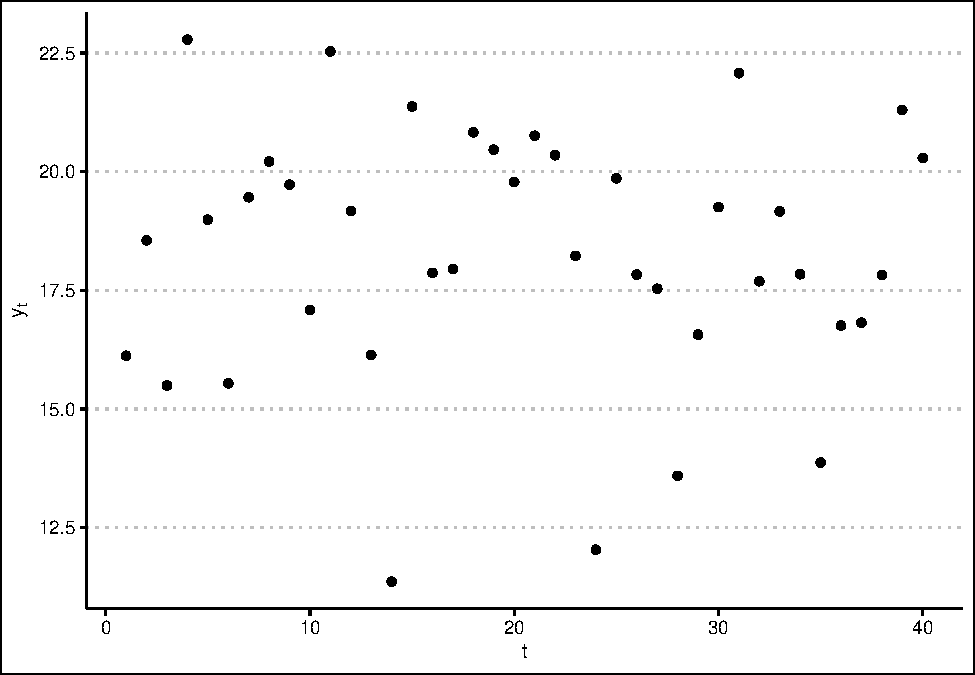
\includegraphics{graphics/unnamed-chunk-57-1.pdf}

Just by visual inspection, there doesn't \emph{seem} to be much of a trend.

Fitting a linear model to the data and plotting the regression line reveals a very shallow downward trend:

\begin{Shaded}
\begin{Highlighting}[]
\NormalTok{p }\SpecialCharTok{+} \FunctionTok{geom\_smooth}\NormalTok{(}\AttributeTok{method =} \StringTok{"lm"}\NormalTok{, }\AttributeTok{se =} \ConstantTok{FALSE}\NormalTok{)}
\end{Highlighting}
\end{Shaded}

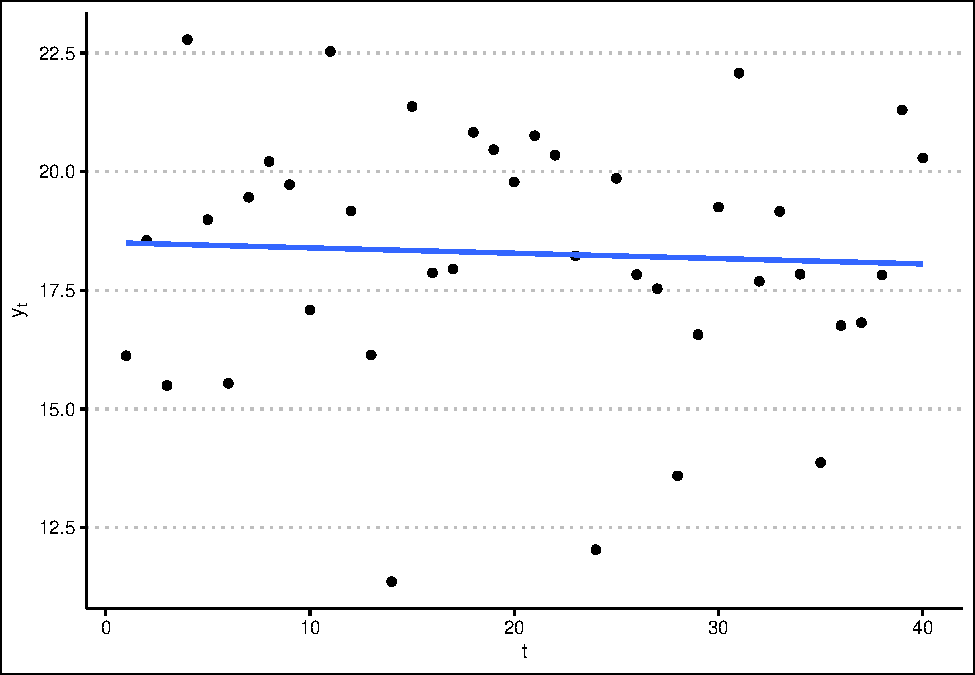
\includegraphics{graphics/unnamed-chunk-58-1.pdf}

Hmmm. Is this trend ``real''? Or did it just happen that, by random chance, the data later in the series happen to have slightly lower values on average than those generated earlier?

This question is very typical of those that arise in the challenge of \emph{model selection}, i.e., of choosing the model that best explains the data generating process. It is sometimes difficult to tell whether a pattern we observe in our data corresponds to a real feature of the underlying process, or if the feature is instead a kind of illusion --- one that just happened to emerge from the particular data we observe, due to random chance, but that would not necessarily be observed from another sample of data drawn from the same process.

We could (with caution) test the statistical significance of the trend term:

\begin{Shaded}
\begin{Highlighting}[]
\NormalTok{y\_tbl }\SpecialCharTok{\%\textgreater{}\%} \FunctionTok{lm}\NormalTok{(y }\SpecialCharTok{\textasciitilde{}}\NormalTok{ t, }\AttributeTok{data =}\NormalTok{ .) }\OtherTok{{-}\textgreater{}}\NormalTok{ temp.lm}

\FunctionTok{print}\NormalTok{(temp.lm)}
\end{Highlighting}
\end{Shaded}

\begin{verbatim}
## 
## Call:
## lm(formula = y ~ t, data = .)
## 
## Coefficients:
## (Intercept)            t  
##    18.50754     -0.01129
\end{verbatim}

\begin{Shaded}
\begin{Highlighting}[]
\FunctionTok{coef}\NormalTok{(temp.lm)}
\end{Highlighting}
\end{Shaded}

\begin{verbatim}
## (Intercept)           t 
## 18.50754230 -0.01129092
\end{verbatim}

\hypertarget{no-autocorrelation}{%
\subsection{No autocorrelation}\label{no-autocorrelation}}

\begin{itemize}
\item
  Temperatures are assumed to be \emph{independent} from one year to the next. In particular, there is no \emph{autocorrelation}. Knowing that one year's temperature was unusually high (say) provides no information about the likelihood that next year's temperature will also be unusually high. Inter-annual climate cycles (e.g., due to \(El\ Ni\tilde{n}o\)) are ruled out.
\item
  Temperature variations around the long-run average are assumed to be \emph{identically distributed}. This assumption rules out the possibility that variance is, say, greater when temperatures are higher than when they are lower. Nor do they grow over time.
\end{itemize}

\hypertarget{the-normal-linear-model}{%
\chapter{The normal linear model}\label{the-normal-linear-model}}

\[ y_t = \beta_0 + \beta_1 x_t + \varepsilon_t \]

\hypertarget{assumptions-of-the-linear-model}{%
\section{Assumptions of the linear model}\label{assumptions-of-the-linear-model}}

\begin{itemize}
\item
  Relationship between predictor \(x\) and predictand \(y\) is linear.
\item
  Both \(x\) and \(y\) are known, observed without error.
\item
  Errors have mean zero.
\item
  Errors are independent of each other.\\
\item
  Errors are uncorrelated with predictor variables \(x_t\).
\end{itemize}

Often, assume stronger additional conditions that errors are \emph{independent, identically normally distributed}: for all \(t\), \(\varepsilon_t \sim N(0, \sigma^2)\). for a constant \(\sigma^2\).

In compact vector and matrix notation, we may write:

\[ 
Y = X \beta + \varepsilon,
\quad \text{where $\varepsilon \sim N(0, \sigma^2 I_T)$} 
\]

Readings: FPP, Section 7.1

\hypertarget{examples-of-the-normal-linear-model}{%
\section{Examples of the normal linear model}\label{examples-of-the-normal-linear-model}}

\hypertarget{ordinary-least-squares-estimation}{%
\chapter{Ordinary least squares estimation}\label{ordinary-least-squares-estimation}}

Regression coefficients \(\beta\) and error variance \(\sigma^2\) are unobserved: their values must be estimated from the data. Various estimation techniques may be used.

\hypertarget{assignment-project-proposal}{%
\chapter{Assignment: Project proposal}\label{assignment-project-proposal}}

In this assignment you will develop your initial concept note into a draft of a full project proposal. Treat this assignment as a ``dry run'' for developing a proposal for a grant or fellowship application, or for your Ph.D.~prospectus.

Your proposal should include at least the following sections and information.

\textbf{Front matter:} Descriptive title, your name, date, reference to ``SYS 5581 Time Series \& Forecasting, Spring 2021''.

\textbf{Abstract:} A very brief summary of the project.

\hypertarget{introduction}{%
\section{Introduction}\label{introduction}}

Give a narrative description of the problem you are addressing, and the methods you will use to address it. Provide context:

\begin{itemize}
\tightlist
\item
  What is the question you are attempting to answer?
\item
  Why is this question important? (Who cares?)
\item
  How will you go about attempting to answer this question?
\end{itemize}

This work addresses the question: Why do people not use probabilistic forecasts for decision-making?

\hypertarget{the-data-and-the-data-generating-process}{%
\section{The data and the data-generating process}\label{the-data-and-the-data-generating-process}}

Describe the data set you will be analyzing, and where it comes from, how it was generated and collected. Identify the source of the data. Give a narrative description of the data-generating process: this piece is critical.

Since these will be time series data: identify the frequency of the data series (e.g., hourly, monthly), and the period of record.

\hypertarget{exploratory-data-analysis}{%
\section{Exploratory data analysis}\label{exploratory-data-analysis}}

Provide a brief example of the data, showing how they are structured.

\hypertarget{plot-the-time-series.}{%
\section{Plot the time series.}\label{plot-the-time-series.}}

\hypertarget{perform-and-report-the-results-of-other-exploratory-data-analysis}{%
\section{Perform and report the results of other exploratory data analysis}\label{perform-and-report-the-results-of-other-exploratory-data-analysis}}

\hypertarget{stl-decomposition}{%
\subsection{STL decomposition}\label{stl-decomposition}}

\begin{Shaded}
\begin{Highlighting}[]
\NormalTok{vaelsales\_tbl\_ts }\SpecialCharTok{\%\textgreater{}\%}
  \FunctionTok{model}\NormalTok{(}\FunctionTok{STL}\NormalTok{(sales\_GWh }\SpecialCharTok{\textasciitilde{}} \FunctionTok{trend}\NormalTok{(}\AttributeTok{window=}\DecValTok{21}\NormalTok{) }\SpecialCharTok{+} \FunctionTok{season}\NormalTok{(}\AttributeTok{window=}\StringTok{\textquotesingle{}periodic\textquotesingle{}}\NormalTok{), }\AttributeTok{robust =} \ConstantTok{TRUE}\NormalTok{)) }\SpecialCharTok{\%\textgreater{}\%}
  \FunctionTok{components}\NormalTok{() }\SpecialCharTok{\%\textgreater{}\%}
  \FunctionTok{autoplot}\NormalTok{()}
\end{Highlighting}
\end{Shaded}

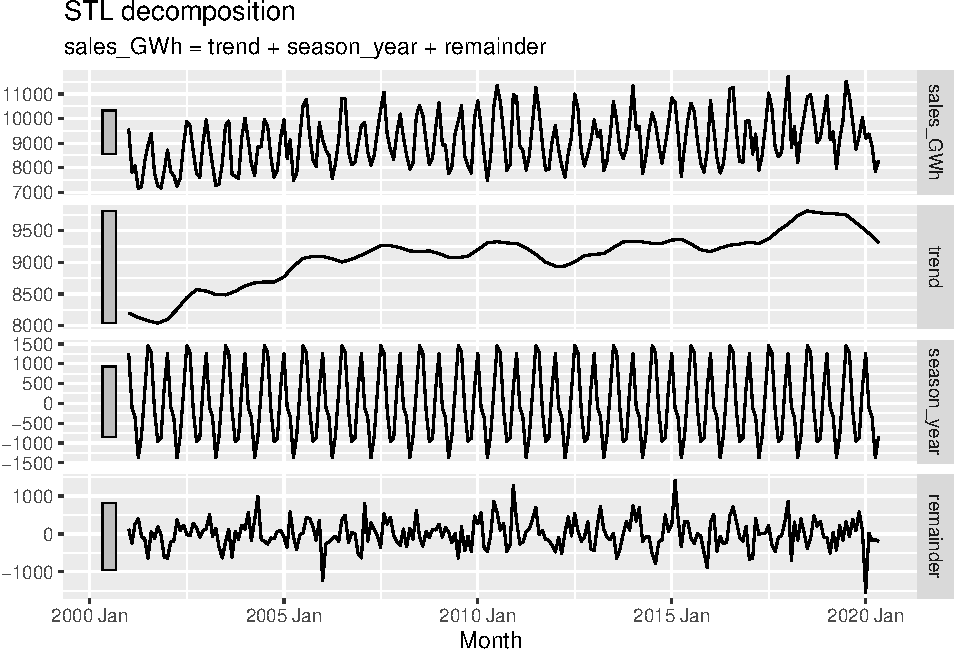
\includegraphics{graphics/perform additive STL decomposition of the VA electricity sales time series 2-1.pdf}

\begin{Shaded}
\begin{Highlighting}[]
\NormalTok{vaelsales\_tbl\_ts }\SpecialCharTok{\%\textgreater{}\%}
  \FunctionTok{mutate}\NormalTok{(}\AttributeTok{ln\_sales\_GWh =} \FunctionTok{log}\NormalTok{(sales\_GWh)) }\SpecialCharTok{\%\textgreater{}\%}
  \FunctionTok{model}\NormalTok{(}\FunctionTok{STL}\NormalTok{(ln\_sales\_GWh }\SpecialCharTok{\textasciitilde{}} \FunctionTok{trend}\NormalTok{(}\AttributeTok{window=}\DecValTok{21}\NormalTok{) }\SpecialCharTok{+} \FunctionTok{season}\NormalTok{(}\AttributeTok{window=}\StringTok{\textquotesingle{}periodic\textquotesingle{}}\NormalTok{),}
    \AttributeTok{robust =} \ConstantTok{TRUE}\NormalTok{)) }\SpecialCharTok{\%\textgreater{}\%}
  \FunctionTok{components}\NormalTok{() }\SpecialCharTok{\%\textgreater{}\%}
  \FunctionTok{autoplot}\NormalTok{()}
\end{Highlighting}
\end{Shaded}

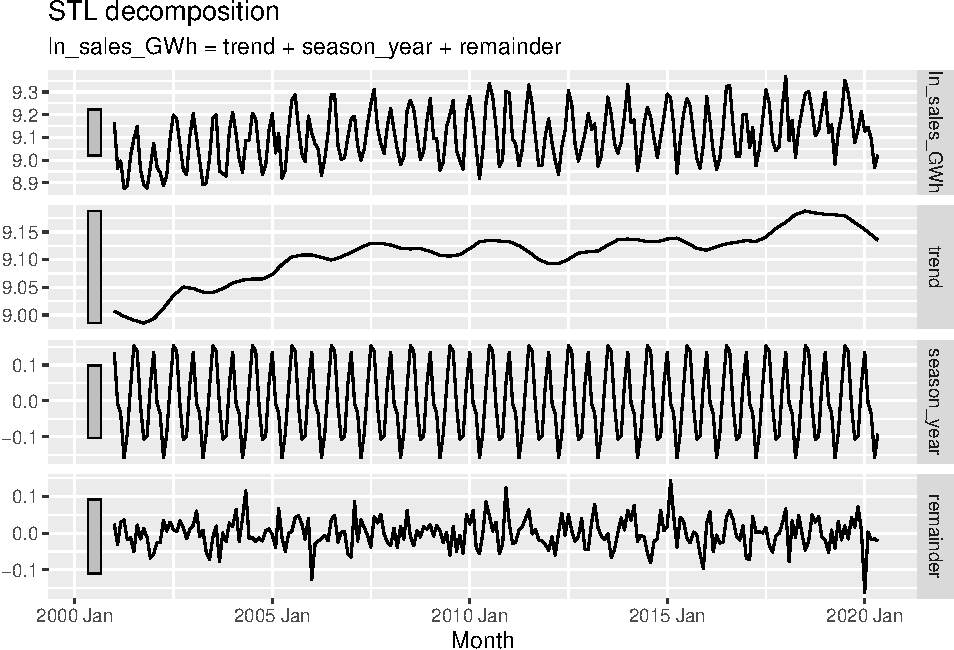
\includegraphics{graphics/perform multiplicative STL decomposition of the VA electricity sales time series 2-1.pdf}

\begin{Shaded}
\begin{Highlighting}[]
\NormalTok{vaelsales\_tbl\_ts }\SpecialCharTok{\%\textgreater{}\%} \FunctionTok{features}\NormalTok{(sales\_GWh, feat\_stl)}
\end{Highlighting}
\end{Shaded}

\begin{verbatim}
## # A tibble: 1 x 9
##   trend_strength seasonal_strength_~ seasonal_peak_y~ seasonal_trough~ spikiness
##            <dbl>               <dbl>            <dbl>            <dbl>     <dbl>
## 1          0.609               0.869                7                4   747395.
## # ... with 4 more variables: linearity <dbl>, curvature <dbl>,
## #   stl_e_acf1 <dbl>, stl_e_acf10 <dbl>
\end{verbatim}

\begin{Shaded}
\begin{Highlighting}[]
\NormalTok{vaelsales\_tbl\_ts }\SpecialCharTok{\%\textgreater{}\%} \FunctionTok{features}\NormalTok{(sales\_GWh, }\FunctionTok{feature\_set}\NormalTok{(}\AttributeTok{pkgs=}\StringTok{"feasts"}\NormalTok{))}
\end{Highlighting}
\end{Shaded}

\begin{verbatim}
## # A tibble: 1 x 47
##   trend_strength seasonal_strength_~ seasonal_peak_y~ seasonal_trough~ spikiness
##            <dbl>               <dbl>            <dbl>            <dbl>     <dbl>
## 1          0.609               0.869                7                4   747395.
## # ... with 42 more variables: linearity <dbl>, curvature <dbl>,
## #   stl_e_acf1 <dbl>, stl_e_acf10 <dbl>, acf1 <dbl>, acf10 <dbl>,
## #   diff1_acf1 <dbl>, diff1_acf10 <dbl>, diff2_acf1 <dbl>, diff2_acf10 <dbl>,
## #   season_acf1 <dbl>, pacf5 <dbl>, diff1_pacf5 <dbl>, diff2_pacf5 <dbl>,
## #   season_pacf <dbl>, zero_run_mean <dbl>, nonzero_squared_cv <dbl>,
## #   zero_start_prop <dbl>, zero_end_prop <dbl>, lambda_guerrero <dbl>,
## #   kpss_stat <dbl>, kpss_pvalue <dbl>, pp_stat <dbl>, pp_pvalue <dbl>, ...
\end{verbatim}

\hypertarget{fitting-data-to-simple-models-1}{%
\subsection{Fitting data to simple models}\label{fitting-data-to-simple-models-1}}

\begin{Shaded}
\begin{Highlighting}[]
\NormalTok{global\_economy }\SpecialCharTok{\%\textgreater{}\%} \FunctionTok{model}\NormalTok{(}\AttributeTok{trend\_model =} \FunctionTok{TSLM}\NormalTok{(GDP }\SpecialCharTok{\textasciitilde{}} \FunctionTok{trend}\NormalTok{())) }\OtherTok{{-}\textgreater{}}\NormalTok{ fit}

\NormalTok{fit}
\end{Highlighting}
\end{Shaded}

\begin{verbatim}
## # A mable: 263 x 2
## # Key:     Country [263]
##    Country             trend_model
##    <fct>                   <model>
##  1 Afghanistan              <TSLM>
##  2 Albania                  <TSLM>
##  3 Algeria                  <TSLM>
##  4 American Samoa           <TSLM>
##  5 Andorra                  <TSLM>
##  6 Angola                   <TSLM>
##  7 Antigua and Barbuda      <TSLM>
##  8 Arab World               <TSLM>
##  9 Argentina                <TSLM>
## 10 Armenia                  <TSLM>
## # ... with 253 more rows
\end{verbatim}

\begin{Shaded}
\begin{Highlighting}[]
\NormalTok{fit }\SpecialCharTok{\%\textgreater{}\%} \FunctionTok{filter}\NormalTok{(Country }\SpecialCharTok{==} \StringTok{"Sweden"}\NormalTok{) }\SpecialCharTok{\%\textgreater{}\%} \FunctionTok{residuals}\NormalTok{()}
\end{Highlighting}
\end{Shaded}

\begin{verbatim}
## # A tsibble: 58 x 4 [1Y]
## # Key:       Country, .model [1]
##    Country .model       Year       .resid
##    <fct>   <chr>       <dbl>        <dbl>
##  1 Sweden  trend_model  1960 79973991821.
##  2 Sweden  trend_model  1961 71110300270.
##  3 Sweden  trend_model  1962 62306636078.
##  4 Sweden  trend_model  1963 53581309752.
##  5 Sweden  trend_model  1964 45596438566.
##  6 Sweden  trend_model  1965 37551535271.
##  7 Sweden  trend_model  1966 29425266377.
##  8 Sweden  trend_model  1967 21418661066.
##  9 Sweden  trend_model  1968 12930653974.
## 10 Sweden  trend_model  1969  5268492989.
## # ... with 48 more rows
\end{verbatim}

\begin{Shaded}
\begin{Highlighting}[]
\NormalTok{fit }\SpecialCharTok{\%\textgreater{}\%} \FunctionTok{filter}\NormalTok{(Country }\SpecialCharTok{==} \StringTok{"Sweden"}\NormalTok{) }\SpecialCharTok{\%\textgreater{}\%} \FunctionTok{residuals}\NormalTok{() }\SpecialCharTok{\%\textgreater{}\%} \FunctionTok{autoplot}\NormalTok{(.resid)}
\end{Highlighting}
\end{Shaded}

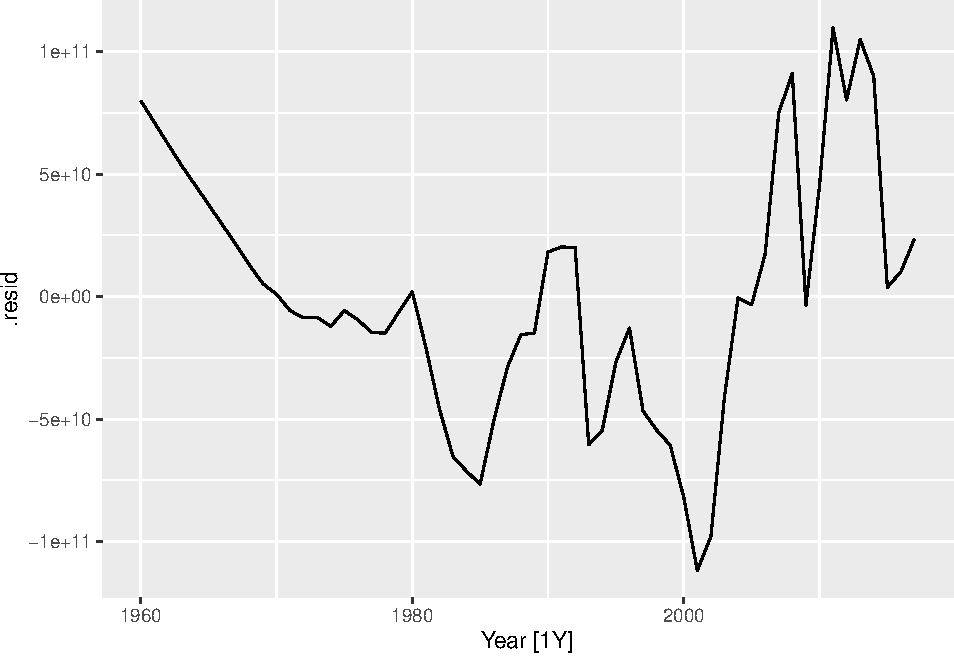
\includegraphics{graphics/unnamed-chunk-64-1.pdf}

\hypertarget{work-with-lngdp-1}{%
\subsection{Work with ln(GDP)}\label{work-with-lngdp-1}}

\begin{Shaded}
\begin{Highlighting}[]
\NormalTok{global\_economy }\SpecialCharTok{\%\textgreater{}\%}
  \FunctionTok{filter}\NormalTok{(Country}\SpecialCharTok{==}\StringTok{"Sweden"}\NormalTok{) }\SpecialCharTok{\%\textgreater{}\%}
  \FunctionTok{autoplot}\NormalTok{(}\FunctionTok{log}\NormalTok{(GDP)) }\SpecialCharTok{+}
  \FunctionTok{ggtitle}\NormalTok{(}\StringTok{"ln(GDP) for Sweden"}\NormalTok{) }\SpecialCharTok{+} \FunctionTok{ylab}\NormalTok{(}\StringTok{"$US billions"}\NormalTok{)}
\end{Highlighting}
\end{Shaded}

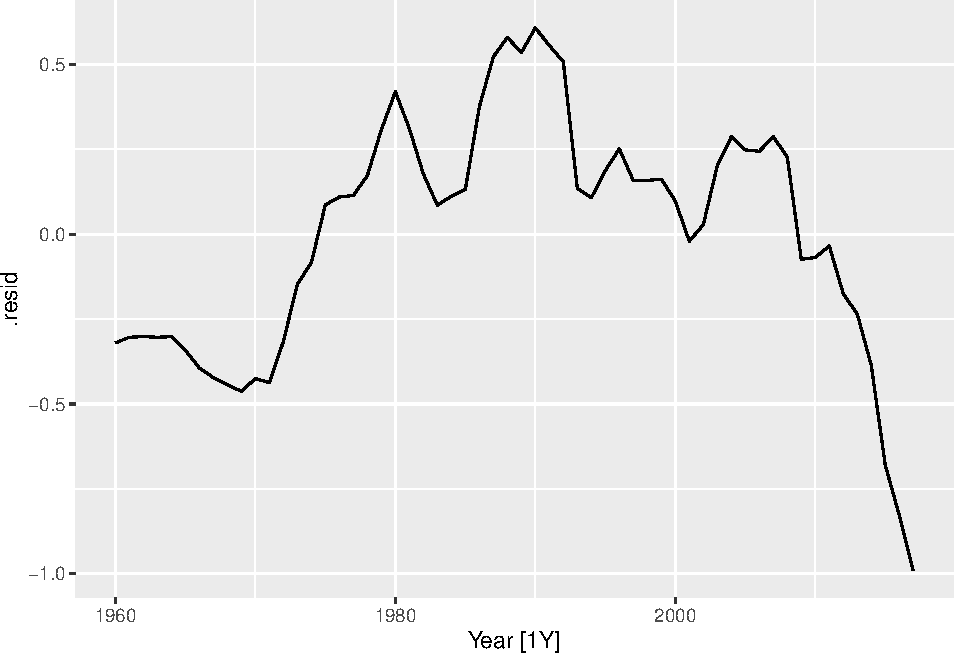
\includegraphics{graphics/unnamed-chunk-65-1.pdf}

\begin{Shaded}
\begin{Highlighting}[]
\NormalTok{global\_economy }\SpecialCharTok{\%\textgreater{}\%}
  \FunctionTok{model}\NormalTok{(}\AttributeTok{trend\_model =} \FunctionTok{TSLM}\NormalTok{(}\FunctionTok{log}\NormalTok{(GDP) }\SpecialCharTok{\textasciitilde{}} \FunctionTok{trend}\NormalTok{())) }\OtherTok{{-}\textgreater{}}\NormalTok{ logfit}
\end{Highlighting}
\end{Shaded}

\begin{Shaded}
\begin{Highlighting}[]
\NormalTok{logfit }\SpecialCharTok{\%\textgreater{}\%} \FunctionTok{filter}\NormalTok{(Country }\SpecialCharTok{==} \StringTok{"Sweden"}\NormalTok{) }\SpecialCharTok{\%\textgreater{}\%} \FunctionTok{residuals}\NormalTok{() }\SpecialCharTok{\%\textgreater{}\%} \FunctionTok{autoplot}\NormalTok{()}
\end{Highlighting}
\end{Shaded}

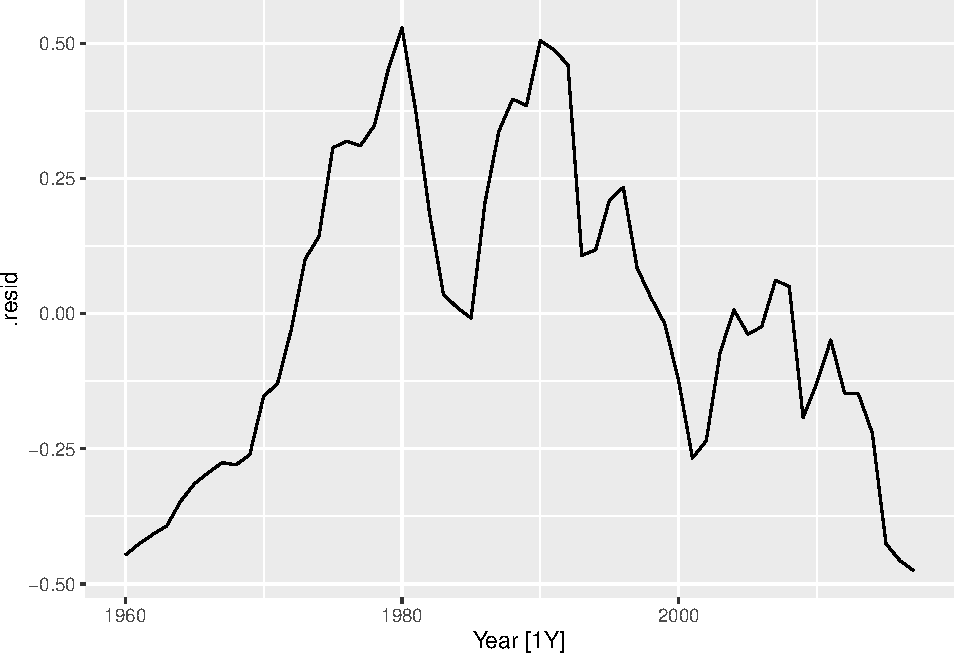
\includegraphics{graphics/unnamed-chunk-67-1.pdf}

\begin{Shaded}
\begin{Highlighting}[]
\NormalTok{global\_economy }\SpecialCharTok{\%\textgreater{}\%} \FunctionTok{model}\NormalTok{(}\AttributeTok{trend\_model =} \FunctionTok{TSLM}\NormalTok{(}\FunctionTok{log}\NormalTok{(GDP) }\SpecialCharTok{\textasciitilde{}} \FunctionTok{log}\NormalTok{(Population))) }\OtherTok{{-}\textgreater{}}\NormalTok{ fit3}

\NormalTok{fit3 }\SpecialCharTok{\%\textgreater{}\%} \FunctionTok{filter}\NormalTok{(Country }\SpecialCharTok{==} \StringTok{"Sweden"}\NormalTok{) }\SpecialCharTok{\%\textgreater{}\%} \FunctionTok{residuals}\NormalTok{() }\SpecialCharTok{\%\textgreater{}\%} \FunctionTok{autoplot}\NormalTok{()}
\end{Highlighting}
\end{Shaded}

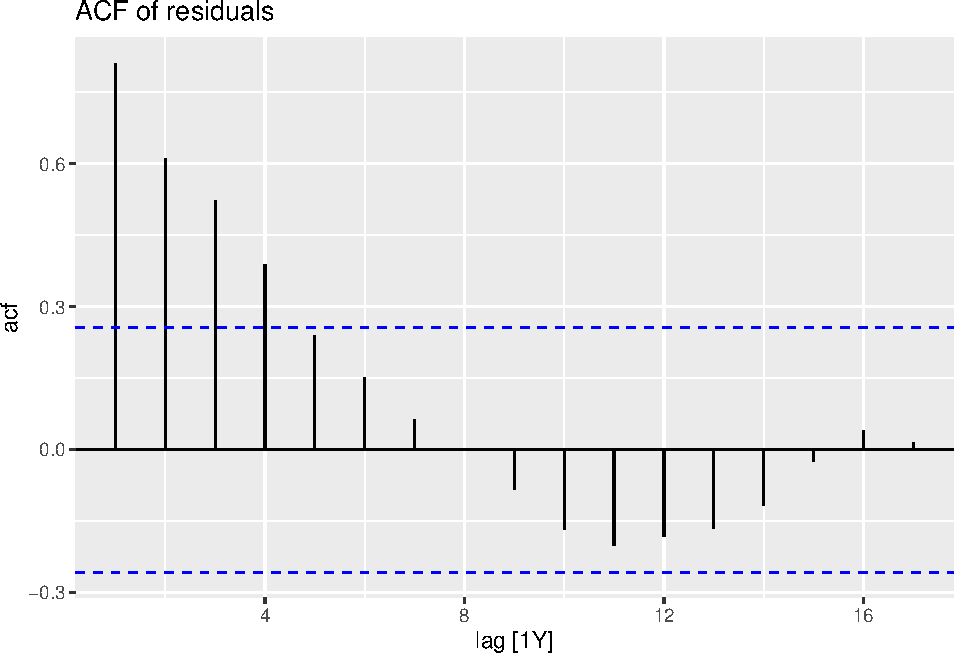
\includegraphics{graphics/unnamed-chunk-68-1.pdf}

\hypertarget{statistical-model}{%
\section{Statistical model}\label{statistical-model}}

\hypertarget{formal-model-of-data-generating-process}{%
\subsection{Formal model of data-generating process}\label{formal-model-of-data-generating-process}}

Write down an equation (or set of equations) that represent the data-generating process formally.

If applicable: describe any transformations of the data (e.g., differencing, taking logs) you need to make to get the data into a form (e.g., linear) ready for numerical analysis.

What kind of process is it? \(AR(p)\)? White noise with drift? Something else?

Write down an equation expressing each realization of the stochastic process \(y_t\) as a function of other observed data (which could include lagged values of \(y\)), unobserved parameters (\(\beta\)), and an error term (\(\varepsilon_t\)). Ex:

\[y = X\cdot\beta + \varepsilon\] Add a model of the error process. Ex: \(\varepsilon \sim N(0, \sigma^2 I_T)\).

\hypertarget{discussion-of-the-statistical-model}{%
\subsection{Discussion of the statistical model}\label{discussion-of-the-statistical-model}}

Describe how the formal statistical model captures and aligns with the narrative of the data-generating process. Flag any statistical challenges raised by the data generating process, e.g.~selection bias; survivorship bias; omitted variables bias, etc.

\hypertarget{plan-for-data-analysis}{%
\section{Plan for data analysis}\label{plan-for-data-analysis}}

Describe what information you wish to extract from the data. Do you wish to\ldots{} estimate the values of the unobserved model parameters? create a tool for forecasting? estimate the exceedance probabilities for future realizations of \(y_t\)?

Describe your plan for getting this information. OLS regression? Some other statistical technique?

If you can: describe briefly which computational tools you will use (e.g., R), and which packages you expect to draw on.

\hypertarget{submission-requirements}{%
\section{Submission requirements}\label{submission-requirements}}

Prepare your proposal using Markdown . (You may find it useful to generate your Markdown file from some other tool, e.g.~R Markdown in R Studio.) Submit your proposal by pushing it to your repo within the course organization on Github. When your proposal is ready, notify the instructor by also creating a submission for this assignment on Collab. Please also upload a PDF version of your proposal to Collab as part of your submission.

\hypertarget{comment}{%
\section{Comment}\label{comment}}

Depending on your prior experience, you may find this assignment challenging. Treat this assignment as an opportunity to make progress on your own research program. Make your proposal as complete as you can. But note that this assignment is merely the First Draft. You will have more opportunity to refine your work over the next two months, in consultation with the instructor, your advisor, and your classmates.

\hypertarget{references}{%
\section{References}\label{references}}

\hypertarget{part-model-evaluation}{%
\part{Model evaluation}\label{part-model-evaluation}}

\hypertarget{evaluating-model-residuals}{%
\chapter{Evaluating model residuals}\label{evaluating-model-residuals}}

\hypertarget{model-residuals-vs.-forecast-errors-1}{%
\section{Model residuals vs.~forecast errors}\label{model-residuals-vs.-forecast-errors-1}}

Model residuals:

Your data: \(y_1, y_2, \ldots, y_T\)

Fitted values: \(\hat{y}_1, \hat{y}_2, \ldots, \hat{y}_T\)

Model residuals: \(e_t = y_t - \hat{y}_t\)

Forecast errors:

\begin{Shaded}
\begin{Highlighting}[]
\FunctionTok{augment}\NormalTok{(fit)}
\end{Highlighting}
\end{Shaded}

\begin{verbatim}
## # A tsibble: 15,150 x 7 [1Y]
## # Key:       Country, .model [263]
##    Country     .model       Year         GDP      .fitted      .resid     .innov
##    <fct>       <chr>       <dbl>       <dbl>        <dbl>       <dbl>      <dbl>
##  1 Afghanistan trend_model  1960  537777811. -1587934559. 2125712370.     2.13e9
##  2 Afghanistan trend_model  1961  548888896. -1281158073. 1830046968.     1.83e9
##  3 Afghanistan trend_model  1962  546666678.  -974381586. 1521048264.     1.52e9
##  4 Afghanistan trend_model  1963  751111191.  -667605100. 1418716291.     1.42e9
##  5 Afghanistan trend_model  1964  800000044.  -360828613. 1160828658.     1.16e9
##  6 Afghanistan trend_model  1965 1006666638.   -54052127. 1060718765.     1.06e9
##  7 Afghanistan trend_model  1966 1399999967.   252724359. 1147275607.     1.15e9
##  8 Afghanistan trend_model  1967 1673333418.   559500846. 1113832572.     1.11e9
##  9 Afghanistan trend_model  1968 1373333367.   866277332.  507056034.     5.07e8
## 10 Afghanistan trend_model  1969 1408888922.  1173053819.  235835103.     2.36e8
## # ... with 15,140 more rows
\end{verbatim}

\begin{Shaded}
\begin{Highlighting}[]
\FunctionTok{augment}\NormalTok{(fit) }\SpecialCharTok{\%\textgreater{}\%} \FunctionTok{filter}\NormalTok{(Country }\SpecialCharTok{==} \StringTok{"Sweden"}\NormalTok{) }\SpecialCharTok{\%\textgreater{}\%}
  \FunctionTok{ggplot}\NormalTok{(}\FunctionTok{aes}\NormalTok{(}\AttributeTok{x =}\NormalTok{ .resid)) }\SpecialCharTok{+}
  \FunctionTok{geom\_histogram}\NormalTok{(}\AttributeTok{bins =} \DecValTok{20}\NormalTok{) }\SpecialCharTok{+}
  \FunctionTok{ggtitle}\NormalTok{(}\StringTok{"Histogram of residuals"}\NormalTok{)}
\end{Highlighting}
\end{Shaded}

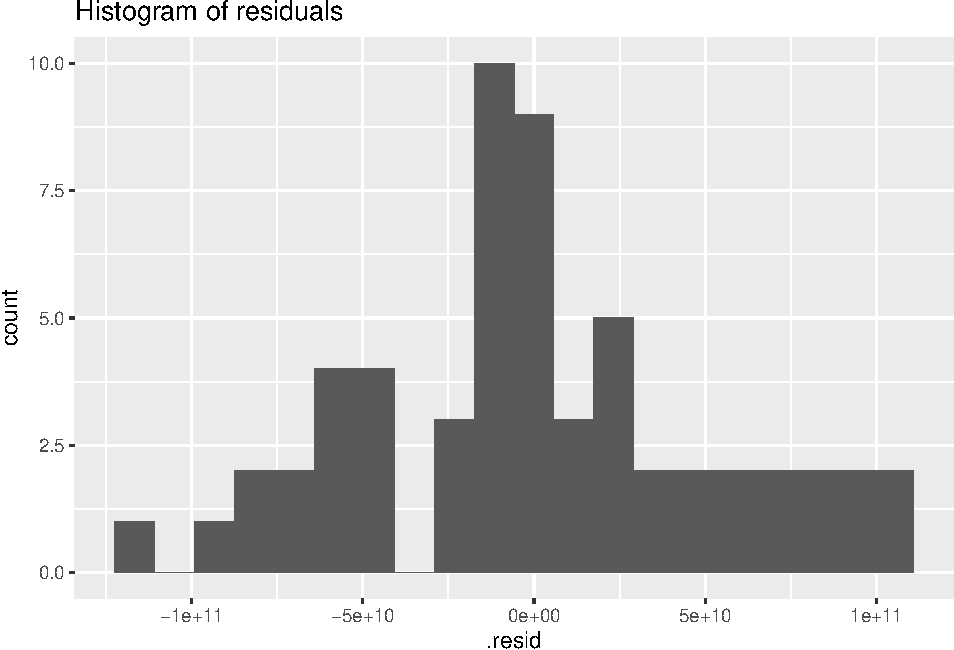
\includegraphics{graphics/unnamed-chunk-70-1.pdf}

\hypertarget{are-the-model-residuals-auto-correlated-1}{%
\section{Are the model residuals auto-correlated?}\label{are-the-model-residuals-auto-correlated-1}}

\begin{Shaded}
\begin{Highlighting}[]
\FunctionTok{augment}\NormalTok{(fit) }\SpecialCharTok{\%\textgreater{}\%} \FunctionTok{filter}\NormalTok{(Country }\SpecialCharTok{==} \StringTok{"Sweden"}\NormalTok{) }\OtherTok{{-}\textgreater{}}\NormalTok{ augSweden}

\NormalTok{augSweden }\SpecialCharTok{\%\textgreater{}\%}
  \FunctionTok{ACF}\NormalTok{(.resid) }\SpecialCharTok{\%\textgreater{}\%}
  \FunctionTok{autoplot}\NormalTok{() }\SpecialCharTok{+} \FunctionTok{ggtitle}\NormalTok{(}\StringTok{"ACF of residuals"}\NormalTok{)}
\end{Highlighting}
\end{Shaded}

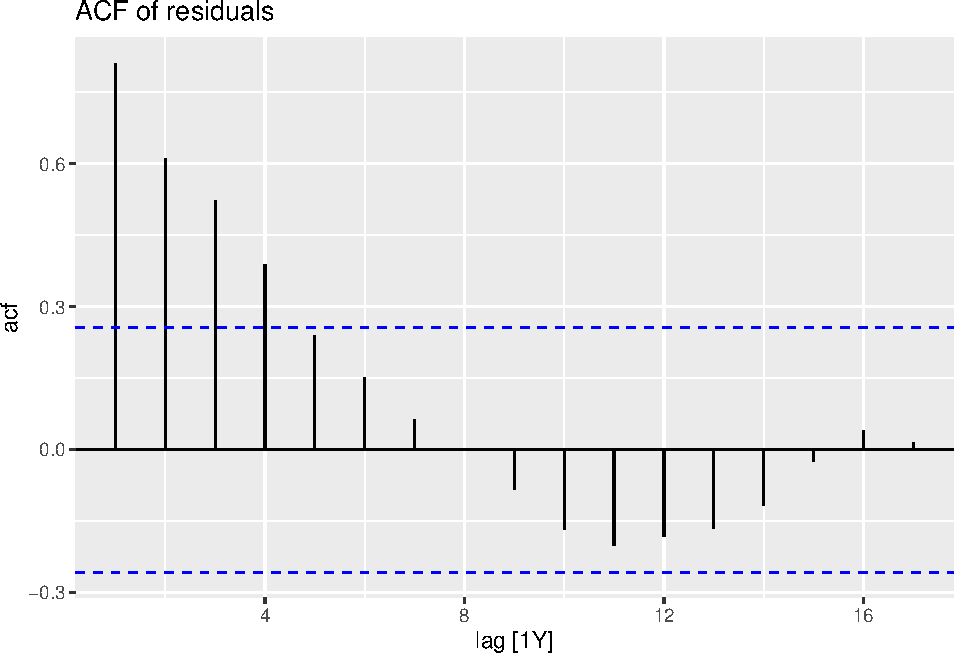
\includegraphics{graphics/unnamed-chunk-71-1.pdf}

\begin{Shaded}
\begin{Highlighting}[]
\FunctionTok{augment}\NormalTok{(fit3) }\SpecialCharTok{\%\textgreater{}\%} \FunctionTok{filter}\NormalTok{(Country }\SpecialCharTok{==} \StringTok{"Sweden"}\NormalTok{) }\OtherTok{{-}\textgreater{}}\NormalTok{ augSweden3}

\NormalTok{augSweden3 }\SpecialCharTok{\%\textgreater{}\%}
  \FunctionTok{ACF}\NormalTok{(.resid) }\SpecialCharTok{\%\textgreater{}\%}
  \FunctionTok{autoplot}\NormalTok{() }\SpecialCharTok{+} \FunctionTok{ggtitle}\NormalTok{(}\StringTok{"ACF of residuals"}\NormalTok{)}
\end{Highlighting}
\end{Shaded}

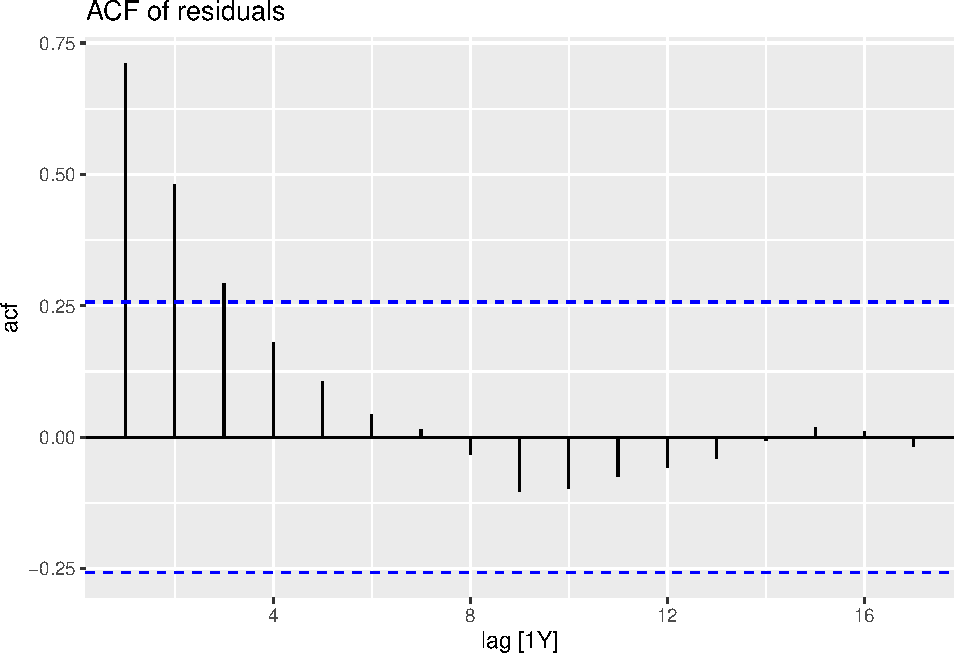
\includegraphics{graphics/unnamed-chunk-72-1.pdf}

\hypertarget{example-gdp-several-models-several-countries}{%
\section{Example: GDP, several models, several countries}\label{example-gdp-several-models-several-countries}}

\begin{Shaded}
\begin{Highlighting}[]
\FunctionTok{library}\NormalTok{(tsibbledata) }\CommentTok{\# Data sets package}

\NormalTok{nordic }\OtherTok{\textless{}{-}} \FunctionTok{c}\NormalTok{(}\StringTok{"Sweden"}\NormalTok{, }\StringTok{"Denmark"}\NormalTok{, }\StringTok{"Norway"}\NormalTok{, }\StringTok{"Finland"}\NormalTok{)}

\NormalTok{(global\_economy }\SpecialCharTok{\%\textgreater{}\%} \FunctionTok{filter}\NormalTok{(Country }\SpecialCharTok{\%in\%}\NormalTok{ nordic) }\OtherTok{{-}\textgreater{}}\NormalTok{ nordic\_economy)}
\end{Highlighting}
\end{Shaded}

\begin{verbatim}
## # A tsibble: 232 x 9 [1Y]
## # Key:       Country [4]
##    Country Code   Year          GDP Growth   CPI Imports Exports Population
##    <fct>   <fct> <dbl>        <dbl>  <dbl> <dbl>   <dbl>   <dbl>      <dbl>
##  1 Denmark DNK    1960  6248946880. NA      8.25    34.3    32.3    4579603
##  2 Denmark DNK    1961  6933842099.  6.38   8.53    32.3    30.0    4611687
##  3 Denmark DNK    1962  7812968114.  5.67   9.16    32.5    28.6    4647727
##  4 Denmark DNK    1963  8316692386.  0.637  9.72    30.8    30.4    4684483
##  5 Denmark DNK    1964  9506678763.  9.27  10.0     32.6    29.9    4722072
##  6 Denmark DNK    1965 10678897387.  4.56  10.6     31.5    29.3    4759012
##  7 Denmark DNK    1966 11721248101.  2.74  11.3     30.8    28.6    4797381
##  8 Denmark DNK    1967 12788479692.  3.42  12.2     30.0    27.3    4835354
##  9 Denmark DNK    1968 13196541952   3.97  13.2     29.7    27.7    4864883
## 10 Denmark DNK    1969 15009384585.  6.32  13.7     30.4    27.6    4891860
## # ... with 222 more rows
\end{verbatim}

\begin{Shaded}
\begin{Highlighting}[]
\NormalTok{nordic\_economy }\SpecialCharTok{\%\textgreater{}\%} \FunctionTok{autoplot}\NormalTok{(GDP)}
\end{Highlighting}
\end{Shaded}

\includegraphics{graphics/unnamed-chunk-74-1.pdf}

\begin{Shaded}
\begin{Highlighting}[]
\NormalTok{fitnord }\OtherTok{\textless{}{-}}\NormalTok{ nordic\_economy }\SpecialCharTok{\%\textgreater{}\%}
  \FunctionTok{model}\NormalTok{(}
    \AttributeTok{trend\_model =} \FunctionTok{TSLM}\NormalTok{(GDP }\SpecialCharTok{\textasciitilde{}} \FunctionTok{trend}\NormalTok{()),}
    \AttributeTok{trend\_model\_ln =} \FunctionTok{TSLM}\NormalTok{(}\FunctionTok{log}\NormalTok{(GDP) }\SpecialCharTok{\textasciitilde{}} \FunctionTok{trend}\NormalTok{()),}
    \AttributeTok{ets =} \FunctionTok{ETS}\NormalTok{(GDP }\SpecialCharTok{\textasciitilde{}} \FunctionTok{trend}\NormalTok{(}\StringTok{"A"}\NormalTok{)),}
    \AttributeTok{arima =} \FunctionTok{ARIMA}\NormalTok{(GDP)}
\NormalTok{  )}

\NormalTok{fitnord}
\end{Highlighting}
\end{Shaded}

\begin{verbatim}
## # A mable: 4 x 5
## # Key:     Country [4]
##   Country trend_model trend_model_ln          ets          arima
##   <fct>       <model>        <model>      <model>        <model>
## 1 Denmark      <TSLM>         <TSLM> <ETS(M,A,N)> <ARIMA(1,1,1)>
## 2 Finland      <TSLM>         <TSLM> <ETS(M,A,N)> <ARIMA(0,1,2)>
## 3 Norway       <TSLM>         <TSLM> <ETS(M,A,N)> <ARIMA(0,1,1)>
## 4 Sweden       <TSLM>         <TSLM> <ETS(M,A,N)> <ARIMA(0,1,2)>
\end{verbatim}

Denmark: ARMA(1,1)

Finland: MA(2)

Norway: MA(1)

Sweden: MA(2)

\begin{Shaded}
\begin{Highlighting}[]
\NormalTok{fitnord }\SpecialCharTok{\%\textgreater{}\%} \FunctionTok{coef}\NormalTok{() }
\end{Highlighting}
\end{Shaded}

\begin{verbatim}
## # A tibble: 39 x 7
##    Country .model         term         estimate std.error statistic   p.value
##    <fct>   <chr>          <chr>           <dbl>     <dbl>     <dbl>     <dbl>
##  1 Denmark trend_model    (Intercept) -5.65e+10   8.75e+9     -6.46  2.70e- 8
##  2 Denmark trend_model    trend()      6.63e+ 9   2.58e+8     25.7   1.14e-32
##  3 Denmark trend_model_ln (Intercept)  2.30e+ 1   8.55e-2    269.    7.68e-89
##  4 Denmark trend_model_ln trend()      7.12e- 2   2.52e-3     28.3   7.68e-35
##  5 Denmark ets            alpha        1.00e+ 0  NA           NA    NA       
##  6 Denmark ets            beta         3.67e- 1  NA           NA    NA       
##  7 Denmark ets            l[0]         4.92e+ 9  NA           NA    NA       
##  8 Denmark ets            b[0]         1.24e+ 9  NA           NA    NA       
##  9 Denmark arima          ar1         -3.90e- 1   2.06e-1     -1.89  6.36e- 2
## 10 Denmark arima          ma1          7.24e- 1   1.43e-1      5.05  4.84e- 6
## # ... with 29 more rows
\end{verbatim}

\begin{Shaded}
\begin{Highlighting}[]
\NormalTok{fitnord }\SpecialCharTok{\%\textgreater{}\%}  \FunctionTok{glance}\NormalTok{()  }
\end{Highlighting}
\end{Shaded}

\begin{verbatim}
## # A tibble: 16 x 21
##    Country .model     r_squared adj_r_squared   sigma2 statistic   p_value    df
##    <fct>   <chr>          <dbl>         <dbl>    <dbl>     <dbl>     <dbl> <int>
##  1 Denmark trend_mod~     0.922         0.920 1.08e+21      660.  1.14e-32     2
##  2 Denmark trend_mod~     0.935         0.933 1.03e- 1      800.  7.68e-35     2
##  3 Denmark ets           NA            NA     1.04e- 2       NA  NA           NA
##  4 Denmark arima         NA            NA     2.41e+20       NA  NA           NA
##  5 Finland trend_mod~     0.914         0.912 7.34e+20      594.  1.70e-31     2
##  6 Finland trend_mod~     0.930         0.929 1.14e- 1      745.  4.96e-34     2
##  7 Finland ets           NA            NA     1.32e- 2       NA  NA           NA
##  8 Finland arima         NA            NA     1.89e+20       NA  NA           NA
##  9 Norway  trend_mod~     0.824         0.821 4.60e+21      262.  8.54e-23     2
## 10 Norway  trend_mod~     0.959         0.958 8.37e- 2     1307.  1.64e-40     2
## 11 Norway  ets           NA            NA     8.23e- 3       NA  NA           NA
## 12 Norway  arima         NA            NA     6.78e+20       NA  NA           NA
## 13 Sweden  trend_mod~     0.919         0.918 2.65e+21      635.  3.07e-32     2
## 14 Sweden  trend_mod~     0.935         0.933 8.19e- 2      800.  7.57e-35     2
## 15 Sweden  ets           NA            NA     1.16e- 2       NA  NA           NA
## 16 Sweden  arima         NA            NA     8.84e+20       NA  NA           NA
## # ... with 13 more variables: log_lik <dbl>, AIC <dbl>, AICc <dbl>, BIC <dbl>,
## #   CV <dbl>, deviance <dbl>, df.residual <int>, rank <int>, MSE <dbl>,
## #   AMSE <dbl>, MAE <dbl>, ar_roots <list>, ma_roots <list>
\end{verbatim}

\begin{Shaded}
\begin{Highlighting}[]
\NormalTok{fitnord }\SpecialCharTok{\%\textgreater{}\%}
  \FunctionTok{accuracy}\NormalTok{() }\SpecialCharTok{\%\textgreater{}\%}
  \FunctionTok{arrange}\NormalTok{(Country, MPE)}
\end{Highlighting}
\end{Shaded}

\begin{verbatim}
## # A tibble: 16 x 11
##    Country .model     .type        ME    RMSE     MAE     MPE   MAPE  MASE RMSSE
##    <fct>   <chr>      <chr>     <dbl>   <dbl>   <dbl>   <dbl>  <dbl> <dbl> <dbl>
##  1 Denmark trend_mod~ Trai~ -1.12e+10 6.89e10 3.67e10  -5.17   28.0  3.34  4.24 
##  2 Denmark ets        Trai~  4.50e+ 7 1.65e10 1.04e10   0.518   7.09 0.946 1.02 
##  3 Denmark arima      Trai~  4.40e+ 9 1.51e10 1.04e10   5.05    8.16 0.945 0.930
##  4 Denmark trend_mod~ Trai~ -2.06e- 6 3.23e10 2.63e10  51.1    80.8  2.40  1.99 
##  5 Finland trend_mod~ Trai~ -8.61e+ 9 5.64e10 2.99e10  -5.53   28.6  2.95  3.82 
##  6 Finland ets        Trai~  1.36e+ 8 1.47e10 9.41e 9   0.795   8.36 0.927 0.996
##  7 Finland arima      Trai~  3.54e+ 9 1.34e10 9.14e 9   5.03    8.92 0.900 0.906
##  8 Finland trend_mod~ Trai~  9.54e- 7 2.66e10 2.21e10  46.1    80.5  2.18  1.80 
##  9 Norway  trend_mod~ Trai~ -1.31e+10 8.20e10 3.51e10  -4.24   24.9  2.24  3.01 
## 10 Norway  ets        Trai~ -5.29e+ 8 2.75e10 1.37e10   0.755   6.94 0.870 1.01 
## 11 Norway  arima      Trai~  4.90e+ 9 2.56e10 1.40e10   5.04    8.11 0.890 0.938
## 12 Norway  trend_mod~ Trai~  2.09e- 6 6.67e10 5.48e10 130.    181.   3.49  2.45 
## 13 Sweden  trend_mod~ Trai~ -1.18e+10 8.23e10 4.79e10  -3.96   23.7  2.25  2.68 
## 14 Sweden  ets        Trai~  1.19e+ 9 3.02e10 1.86e10   0.745   7.64 0.875 0.984
## 15 Sweden  arima      Trai~  8.48e+ 9 2.89e10 2.01e10   5.18    9.37 0.942 0.944
## 16 Sweden  trend_mod~ Trai~  2.10e- 6 5.05e10 3.90e10  29.4    53.3  1.83  1.65 
## # ... with 1 more variable: ACF1 <dbl>
\end{verbatim}

\hypertarget{part-forecasting}{%
\part{Forecasting}\label{part-forecasting}}

\hypertarget{producing-forecasts-1}{%
\chapter{Producing forecasts}\label{producing-forecasts-1}}

\hypertarget{example-gross-domestic-product-data-1}{%
\section{Example: Gross Domestic Product data}\label{example-gross-domestic-product-data-1}}

\begin{Shaded}
\begin{Highlighting}[]
\FunctionTok{library}\NormalTok{(tsibbledata) }\CommentTok{\# Data sets package}
\NormalTok{global\_economy }\SpecialCharTok{\%\textgreater{}\%} \FunctionTok{model}\NormalTok{(}\AttributeTok{trend\_model =} \FunctionTok{TSLM}\NormalTok{(GDP }\SpecialCharTok{\textasciitilde{}} \FunctionTok{trend}\NormalTok{())) }\OtherTok{{-}\textgreater{}}\NormalTok{ fit}
\end{Highlighting}
\end{Shaded}

\begin{Shaded}
\begin{Highlighting}[]
\NormalTok{fit }\SpecialCharTok{\%\textgreater{}\%} \FunctionTok{forecast}\NormalTok{(}\AttributeTok{h =} \StringTok{"3 years"}\NormalTok{) }\OtherTok{{-}\textgreater{}}\NormalTok{ fcast3yrs}

\NormalTok{fcast3yrs}
\end{Highlighting}
\end{Shaded}

\begin{verbatim}
## # A fable: 789 x 5 [1Y]
## # Key:     Country, .model [263]
##    Country        .model       Year                 GDP         .mean
##    <fct>          <chr>       <dbl>              <dist>         <dbl>
##  1 Afghanistan    trend_model  2018 N(1.6e+10, 1.3e+19)  16205101654.
##  2 Afghanistan    trend_model  2019 N(1.7e+10, 1.3e+19)  16511878141.
##  3 Afghanistan    trend_model  2020 N(1.7e+10, 1.3e+19)  16818654627.
##  4 Albania        trend_model  2018 N(1.4e+10, 3.9e+18)  13733734164.
##  5 Albania        trend_model  2019 N(1.4e+10, 3.9e+18)  14166852711.
##  6 Albania        trend_model  2020 N(1.5e+10, 3.9e+18)  14599971258.
##  7 Algeria        trend_model  2018 N(1.6e+11, 9.4e+20) 157895153441.
##  8 Algeria        trend_model  2019 N(1.6e+11, 9.4e+20) 161100952126.
##  9 Algeria        trend_model  2020 N(1.6e+11, 9.4e+20) 164306750811.
## 10 American Samoa trend_model  2018 N(6.8e+08, 1.7e+15)    682475000 
## # ... with 779 more rows
\end{verbatim}

\begin{Shaded}
\begin{Highlighting}[]
\NormalTok{fcast3yrs }\SpecialCharTok{\%\textgreater{}\%} \FunctionTok{filter}\NormalTok{(Country }\SpecialCharTok{==} \StringTok{"Sweden"}\NormalTok{, Year }\SpecialCharTok{==} \DecValTok{2020}\NormalTok{) }\SpecialCharTok{\%\textgreater{}\%} \FunctionTok{str}\NormalTok{()}
\end{Highlighting}
\end{Shaded}

\begin{verbatim}
## fbl_ts [1 x 5] (S3: fbl_ts/tbl_ts/tbl_df/tbl/data.frame)
##  $ Country: Factor w/ 263 levels "Afghanistan",..: 232
##  $ .model : chr "trend_model"
##  $ Year   : num 2020
##  $ GDP    : dist [1:1] 
##   ..$ 3:List of 2
##   .. ..$ mu   : num 5.45e+11
##   .. ..$ sigma: num 5.34e+10
##   .. ..- attr(*, "class")= chr [1:2] "dist_normal" "dist_default"
##   ..@ vars: chr "GDP"
##  $ .mean  : num 5.45e+11
##  - attr(*, "key")= tibble [1 x 3] (S3: tbl_df/tbl/data.frame)
##   ..$ Country: Factor w/ 263 levels "Afghanistan",..: 232
##   ..$ .model : chr "trend_model"
##   ..$ .rows  : list<int> [1:1] 
##   .. ..$ : int 1
##   .. ..@ ptype: int(0) 
##   ..- attr(*, ".drop")= logi TRUE
##  - attr(*, "index")= chr "Year"
##   ..- attr(*, "ordered")= logi TRUE
##  - attr(*, "index2")= chr "Year"
##  - attr(*, "interval")= interval [1:1] 1Y
##   ..@ .regular: logi TRUE
##  - attr(*, "response")= chr "GDP"
##  - attr(*, "dist")= chr "GDP"
##  - attr(*, "model_cn")= chr ".model"
\end{verbatim}

\begin{Shaded}
\begin{Highlighting}[]
\NormalTok{fcast3yrs }\SpecialCharTok{\%\textgreater{}\%} 
  \FunctionTok{filter}\NormalTok{(Country}\SpecialCharTok{==}\StringTok{"Sweden"}\NormalTok{) }\SpecialCharTok{\%\textgreater{}\%}
  \FunctionTok{autoplot}\NormalTok{(global\_economy) }\SpecialCharTok{+}
  \FunctionTok{ggtitle}\NormalTok{(}\StringTok{"GDP for Sweden"}\NormalTok{) }\SpecialCharTok{+} \FunctionTok{ylab}\NormalTok{(}\StringTok{"$US billions"}\NormalTok{)}
\end{Highlighting}
\end{Shaded}

\includegraphics{graphics/visualize forecasts 2-1.pdf}

\hypertarget{communicating-forecast-uncertainty}{%
\chapter{Communicating forecast uncertainty}\label{communicating-forecast-uncertainty}}

\includegraphics{/Users/aas9z/GitRepos/Teaching/time-series/tsf/graphics/forecast_communications/nas-completing_the_forecast-cover_image.jpg}

\hypertarget{the-red-river-flood-of-1997}{%
\section{The Red River Flood of 1997}\label{the-red-river-flood-of-1997}}

\includegraphics{/Users/aas9z/GitRepos/Teaching/time-series/tsf/graphics/forecast_communications/Headline_from_The_Forum_newspaper_April_24_1997.png}

\includegraphics{/Users/aas9z/GitRepos/Teaching/time-series/tsf/graphics/forecast_communications/Deterministic_forecasts_issued_by_NWS_prior_to_the_Red_River_flood_of_1997.png}

\includegraphics{/Users/aas9z/GitRepos/Teaching/time-series/tsf/graphics/forecast_communications/Probabilistic_river_stage_forecast_from_AHPS-SOURCE_NWS.png}

  \bibliography{book.bib,packages.bib}

\end{document}
